
\documentclass[10pt,  english, makeidx, a4paper, titlepage, oneside]{book}
\usepackage{babel}
\usepackage{fancyhdr}
\usepackage{makeidx}
\usepackage{titlesec}
\usepackage{listings}
\lstset{basicstyle=\ttfamily\footnotesize,
	showstringspaces=false,
	commentstyle=\color{red},
	captionpos=b,
	keywordstyle=\color{blue},
	breaklines=true,
	numbers=left
}
\usepackage{subcaption}
\usepackage{dirtree}
\usepackage{booktabs}
\usepackage{hyperref}
\usepackage{tikz}
\usepackage{tikz-timing}
\usetikzlibrary{circuits.logic.US}
\usepackage[most]{tcolorbox}
\usepackage{array}
\usepackage{bytefield}
\usepackage{xcolor}
\usepackage{colortbl}
\usepackage{tabularx}
\usepackage{multirow}
\newenvironment{listato}{\footnotesize}{\normalsize }

%\pagestyle{empty}

\textwidth 15.5cm
\textheight 23cm
\topmargin -1cm
\oddsidemargin 0cm
\linespread{1.1}

\pagestyle{fancy}
\lhead{}
\chead{Microelectronic Systems}
\lfoot{}
\cfoot{}
\rfoot{}
\rhead{\thepage}

\usepackage{graphicx}
\usepackage{amsmath}
\usepackage{amsfonts}
\usepackage{amsthm}
\usepackage{amssymb}
%\oddsidemargin -1.1cm
\usepackage{graphicx}
\usepackage{rotating}
\usepackage{caption}
\usepackage{float}
\usepackage{amsmath}
\usepackage{amssymb}
\usepackage{amsfonts}
\usepackage{amsthm}
%\usepackage{subscript}
\usepackage{empheq}
\usepackage{verbatim}
\usepackage{fancyvrb}
\usepackage{multicol}


\definecolor{LightGreen}{HTML}{E5F1E5}
\definecolor{DarkGreen}{HTML}{377b07}
\newtcolorbox{mybox}{
	enhanced,
	boxrule=0pt,frame hidden,
	borderline west={3pt}{0pt}{DarkGreen},
	colback=LightGreen,
	sharp corners
}
\newtcolorbox{box_implementation_details}{
	enhanced,
	boxrule=0pt,frame hidden,
	borderline west={3pt}{0pt}{DarkGreen},
	colback=lightgray,
	sharp corners
}


\usepackage{xparse} % NewDocumentCommand, IfValueTF, IFBooleanTF

% Reference a bus.
%
% Usage:
%
%     \busref[3::0]{C/BE}    ->   C/BE[3::0]
%     \busref*{AD}           ->   AD#
%     \busref*[3::0]{C/BE}   ->   C/BE[3::0]#
%
\NewDocumentCommand{\busref}{som}{\texttt{%
#3%
\IfValueTF{#2}{[#2]}{}%
\IfBooleanTF{#1}{\#}{}%
}}

% Definisce i colori per il codice in VHDL

\lstdefinestyle{vhdl}{
   language=vhdl,
   frame=none,
   basicstyle=\ttfamily\footnotesize,
   breaklines=true,
   captionpos=b,
   keepspaces=true,
   backgroundcolor=\color{white},
   keywordstyle=[1]\color{blue}\bf,
   keywordstyle=[2]\color{red}\bf,
   keywordstyle=[3]\color{cyan!50}\bf,
   stringstyle=\color{orange},
   commentstyle=\color{gray},
   tabsize=2,
    numbers=left,
   showspaces=false,
   showstringspaces=false,
   showtabs=false,
   moredelim=[s][\textcolor{green}]{component}{is},
   morekeywords=[1]{
      library, use ,all,entty,is,port,in,out,end,architecture,of, body,
      function, variable, begin,and,or,Not,downto,ALL, signal, process, if,
      else, elsif, case, when, then, range, to, component, type, with, select,
      others, constant, inout, buffer, map, true, false, array, subtype, wait,
      wait for, generic, =, <, >, <=, >=, =>,
   },
   alsoletter={=, <, >},
   morekeywords=[2]{
          STD_LOGIC_VECTOR,STD_LOGIC,IEEE,STD_LOGIC_1164, work, local, real,
          math_real, time, NUMERIC_STD,STD_LOGIC_ARITH,STD_LOGIC_UNSIGNED,
          std_logic_vectr, std_logic, ieee, numeric_std, std_ulogic,
          std_logic_1164, natural, bit, bit_vector, signed, unsigned,
          boolean, integer
    },
    morekeywords=[3]{rising_edge, falling_edge, resize, to_signed, to_unsigned},
    morecomment=[l]{--},
    morecomment=[s][\color{orange}]{'}{'},
    numbers=left,
}

\definecolor{dkgreen}{rgb}{0,0.6,0}
\definecolor{gray}{rgb}{0.5,0.5,0.5}
\definecolor{mauve}{rgb}{0.58,0,0.82}

\lstdefinelanguage[mips]{Assembler}{%
  % so listings can detect directives and register names
  alsoletter={.\$},
  % strings, characters, and comments
  morestring=[b]",
  morestring=[b]',
  morecomment=[l]\;,
  % instructions
  morekeywords={[1]abs,abs.d,abs.s,add,add.d,add.s,addi,addiu,addu,%
    and,andi,b,bc1f,bc1t,beq,beqz,bge,bgeu,bgez,bgezal,bgt,bgtu,%
    bgtz,ble,bleu,blez,blt,bltu,bltz,bltzal,bne,bnez,break,c.eq.d,%
    c.eq.s,c.le.d,c.le.s,c.lt.d,c.lt.s,ceil.w.d,ceil.w.s,clo,clz,%
    cvt.d.s,cvt.d.w,cvt.s.d,cvt.s.w,cvt.w.d,cvt.w.s,div,div.d,div.s,%
    divu,eret,floor.w.d,floor.w.s,j,jal,jalr,jr,l.d,l.s,la,lb,lbu,%
    ld,ldc1,lh,lhu,li,ll,lui,lw,lwc1,lwl,lwr,madd,maddu,mfc0,mfc1,%
    mfc1.d,mfhi,mflo,mov.d,mov.s,move,movf,movf.d,movf.s,movn,movn.d,%
    movn.s,movt,movt.d,movt.s,movz,movz.d,movz.s,msub,msubu,mtc0,mtc1,%
    mtc1.d,mthi,mtlo,mul,mul.d,mul.s,mulo,mulou,mult,multu,mulu,neg,%
    neg.d,neg.s,negu,nop,nor,not,or,ori,rem,remu,rol,ror,round.w.d,%
    round.w.s,s.d,s.s,sb,sc,sd,sdc1,seq,sge,sgeu,sgt,sgtu,sh,sle,%
    sleu,sll,sllv,slt,slti,sltiu,sltu,sne,sqrt.d,sqrt.s,sra,srav,srl,%
    srlv,sub,sub.d,sub.s,subi,subiu,subu,sw,swc1,swl,swr,syscall,teq,%
    teqi,tge,tgei,tgeiu,tgeu,tlt,tlti,tltiu,tltu,tne,tnei,trunc.w.d,%
    trunc.w.s,ulh,ulhu,ulw,ush,usw,xor,xori, call, ret, sgei, slei, 
    snei, seqi, sgti, sgeui, sgtui, sltui, slli, srli, srai, addui, lhi,
    subui},
  % assembler directives
  morekeywords={[2].align,.ascii,.asciiz,.byte,.data,.double,.extern,%
    .float,.globl,.half,.kdata,.ktext,.set,.space,.text,.word},
  % register names
  morekeywords={[3]\$0,\$1,\$2,\$3,\$4,\$5,\$6,\$7,\$8,\$9,\$10,\$11,%
    \$12,\$13,\$14,\$15,\$16,\$17,\$18,\$19,\$20,\$21,\$22,\$23,\$24,%
    \$25,\$26,\$27,\$28,\$29,\$30,\$31,%
    \$zero,\$at,\$v0,\$v1,\$a0,\$a1,\$a2,\$a3,\$t0,\$t1,\$t2,\$t3,\$t4,
    \$t5,\$t6,\$t7,\$s0,\$s1,\$s2,\$s3,\$s4,\$s5,\$s6,\$s7,\$t8,\$t9,%
    \$k0,\$k1,\$gp,\$sp,\$fp,\$ra},
}[strings,comments,keywords]

\lstdefinestyle{mips}{ %
  language=[mips]Assembler,       % the language of the code
  basicstyle=\ttfamily\footnotesize,
  numbers=left,                   % where to put the line-numbers
  stepnumber=1,                   % the step between two line-numbers. If it's 1, each line
                                  % will be numbered
  backgroundcolor=\color{white},  % choose the background color. You must add \usepackage{color}
  showspaces=false,               % show spaces adding particular underscores
  showstringspaces=false,         % underline spaces within strings
  showtabs=false,                 % show tabs within strings adding particular underscores
  rulecolor=\color{black},        % if not set, the frame-color may be changed on line-breaks within not-black text (e.g. commens (green here))
  tabsize=4,                      % sets default tabsize to 2 spaces
  captionpos=b,                   % sets the caption-position to bottom
  breaklines=true,                % sets automatic line breaking
  breakatwhitespace=false,        % sets if automatic breaks should only happen at whitespace
  title=\lstname,                 % show the filename of files included with \lstinputlisting;
                                  % also try caption instead of title
  keywordstyle=\color{blue},          % keyword style
  commentstyle=\color{dkgreen},       % comment style
  stringstyle=\color{mauve},         % string literal style
  escapeinside={\%*}{*)},            % if you want to add a comment within your code
  morekeywords={*,...}               % if you want to add more keywords to the set
}


\titleformat{\chapter}[display]
{\normalfont\Large\filcenter\sffamily}
{\titlerule[0.5pt]%
\vspace{1pt}
\titlerule
\vspace{1pc}
\LARGE\MakeUppercase{\chaptertitlename} \thechapter
}
{1pc}
{\titlerule
\vspace{1pc}
\Huge}

\makeindex

\begin{document}

\frontmatter
\begin{titlepage}
\vspace{0cm}
\centerline{

\includegraphics[width=9cm]{./logopoli}} 
\vspace{0.5cm}
\vspace{2.5cm}
\centerline{\huge\sf Microelectronic Systems}
\vspace{1cm}
\centerline{\Huge\sf DLX Microprocessor: Design \& Development}
\bigskip
\centerline{\huge\sf Final Project Report}
\vspace{1cm}
\centerline{\Large Master degree in Computer Engineering}
\bigskip
\centerline{\Large Master degree in Electronics Engineering}
\vspace{4.5cm}
%%%%%%%%%%%%%%%%%%%%%%%%%%%%%%%%%%%%%%%%%%%%%%%%%%%%%%
%
\centerline{\large Referents: Prof. Mariagrazia Graziano, Giovanna Turvani}
\bigskip
\vspace{1cm}
\centerline{\large Authors: group\_16}
\bigskip
\centerline{\large \textbf{Battilana Matteo, La Greca Salvatore Gabriele, Pollo Giovanni}}
%
%%%%%%%%%%%%%%%%%%%%%%%%%%%%%%%%%%%%%%%%%%%%%%%%%%%%%%
\vspace{2cm}
\centerline{\large \today}
\end{titlepage}


\shipout\null

\chapter{Feature}
\begin{center}

\vfill
\begin{tabular}{ l c }
	\textbf{Frequency} & 400 MHz \\ 
	\textbf{Slack} & 0 (MET) \\  
	\textbf{Area} & 35278.24 \\  
	\textbf{Total Dynamic power} & 9.88 mW \\  
	\textbf{Cell Leakage power} & 653.22 $\mu$W
\end{tabular}

\end{center}
\hfill
\\[60pt]
\hfill

\begin{multicols}{2}
\begin{itemize}
\item 32 bit RISC CPU
\item 400 MHz operating frequency
\item Up to 4 GB of Addressable Memories
\item Five stages pipeline
\item Full Hazard Detection \& Control
\item System Tick Timer
\item Enhanced T2 3-level Shifter
\item Hardwired Control Unit
\end{itemize}

\columnbreak

\begin{itemize}
\item Expanded instruction set
\item Fast Subroutine call with Windowing RF
\item Word, Half and Byte addressable Memory
\item Signed/Unsigned multipurpose comparator
\item Advanced Datapath with reduced delay
\item Efficient CLA-Carry Select Adders
\item Enhanced Booth's Multiplier
\end{itemize}
\end{multicols}
\vfill

\tableofcontents
\lstlistoflistings

\mainmatter

\chapter{Introduction}

\section{Abstract}
The goal of this project is to build from scratch a working implementation of a DLX. To achieve the goal, some known blocks, created during laboratories, were used. 

The second step was the design of the Datapath, done in the best possible way to obtain a high optimization and performance level. Some optimization examples that will be explained more in-depth in the document are the use of the P4 adder and the Booth multiplier inside the ALU, the comparator and many others. 

The third step was the design of the control unit. Again, the choice fell on the microprogrammed version that guaranteed the pipeline implementation. To simplify the maintainability of the control unit, some struct-like constructs were used in the VHDL code. 

In the fourth step, very exhaustive testing has been executed. All the proposed asm codes were verified, but some well-known algorithm (bubble sort, Fibonacci and factorial) was written and tested.

Last but not least, the DLX has been synthesized using Synopsis, and a post-synthesis simulation has been executed. 

Thanks to the datapath optimization and the synthesis optimization, the microprocessor proposed in this paper reached a peak speed of 400MHz.  
\section{Workflow}
As many tools we used to automate the working process, they are explained in this section.

The first and most important tool was versioning control. The choice fell on GitHub. Thanks to this, the team managed all versions of the code and stepped back if any problem occurs. In addition to that, team communication and issue management were very straightforward, thanks to the possibilities offered by the tool. Another handy feature was the milestone, which allows the team to be on time and respect deadlines. 

The used programming technique was pair programming, which allows writing code and checking its correctness at the same time. This technique was beneficial under challenging parts of the projects. To exploit pair programming the extension used was Live Share for Visual Studio Code (\url{https://github.com/MicrosoftDocs/live-share}). Indeed, for the more manageable steps, the use of the branches and pull request gave the possibility of parallel working and drastically reduced the presence of conflicts. 

The last thing to point out was the intensive use of scripting to compile VHDL code, simulate it, add waves, and then synthesize. All scripts are reported in the appendix.
\chapter{Hardware Architecture}

\section{Overview}

This DLX is a 32-bit RISC processor with a five-stage pipeline. The external interface is made mainly for memories connection (IRAM, DRAM and a DRAM for the Register File) and the Clock and Reset signals. Inside we find the following blocks:

\begin{itemize}
    \item Control Unit: it receives the fetched instruction from the IR register and starts to output the correct control signals towards all the pipeline stages. Moreover, it receives status signals from all other units about their working status like the comparator result (for branch decision), the status about possible hazards in the pipeline, Register File's Push \& Pop operations under execution, and all the memories readiness. It's in charge of controlling the entire pipeline and stop it in case of hazards or other situations that require a stall.
    \item Decode Unit: part of the decode stage, it is in charge of keeping the status about all registers under usage (for further hazard controls), computation of the new Program Counter (given a Jump or not), data comparison (for branches) and, the most important thing, the operation decode with the dispatch of all the operands towards the right ports of the DataPath.
    \item DataPath: the computational core of the processor. Made of 4 pipeline stages (Instruction Decode, Execution, Memory, Write Back) contains all the units capable of computation. In particular, we have the Register File (that manages all the core registers), the Arithmetic Logic Unit, the Load-Store Unit for data memory management, and other units useful for the correct operation of everything.
    \item IR and PC: two registers that compose the Instruction Fetch stage of the pipeline are in charge of keeping in memory the current instruction under execution and the address for the next instruction to execute, respectively. 
\end{itemize}


\begin{figure}[ht]
    \centering
    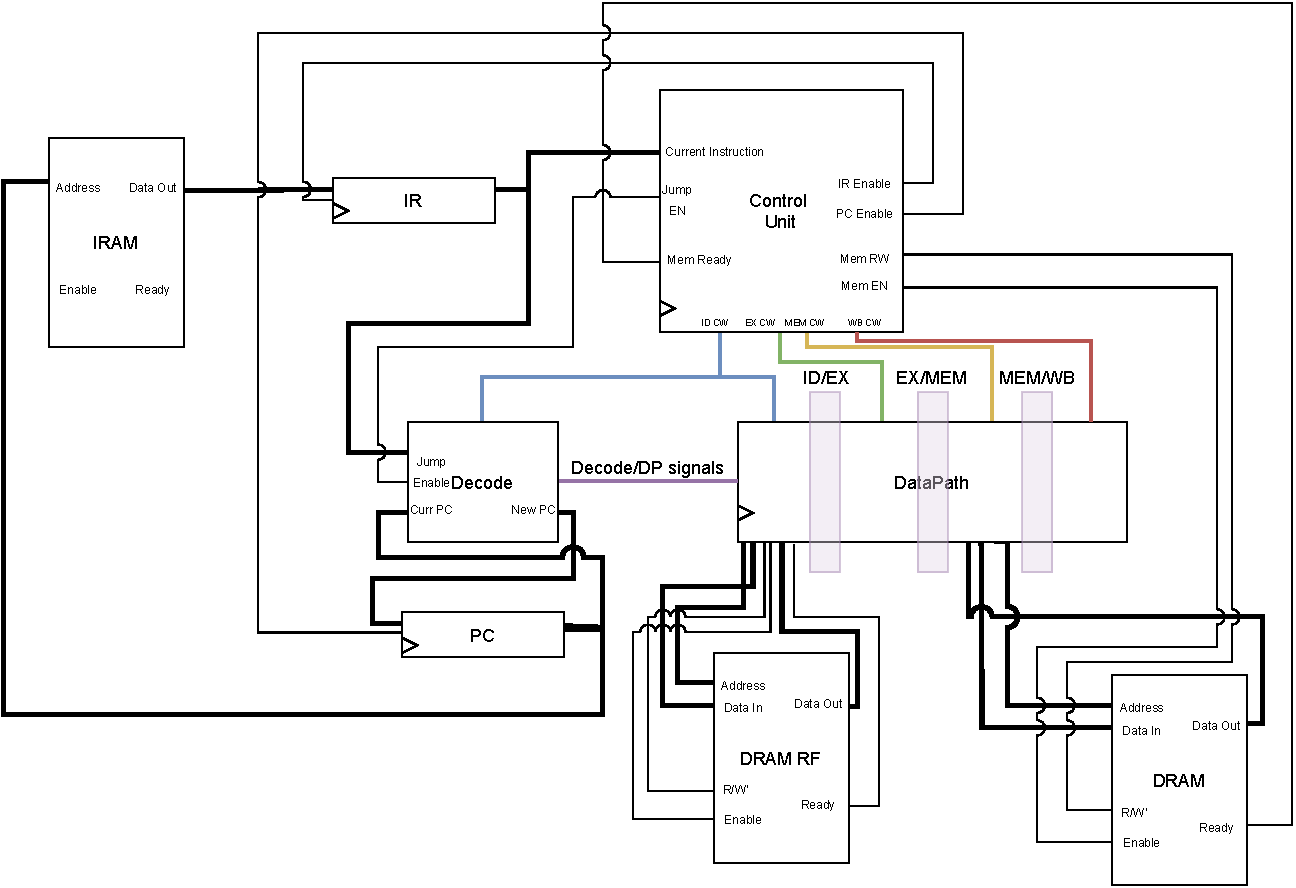
\includegraphics[width=1\textwidth]{chapters/2_dlx/images/DLX.pdf}
    \caption{Schematic of the DLX}
    \label{DLX}
\end{figure} 

\newpage
\section{Pipeline Stages}

To exploit the performance of the DLX processor, a five pipeline stage is implemented. This is done to reduce the overall delay, and different instructions can be processed in various stages simultaneously.

\begin{figure}[H]
    \centering
    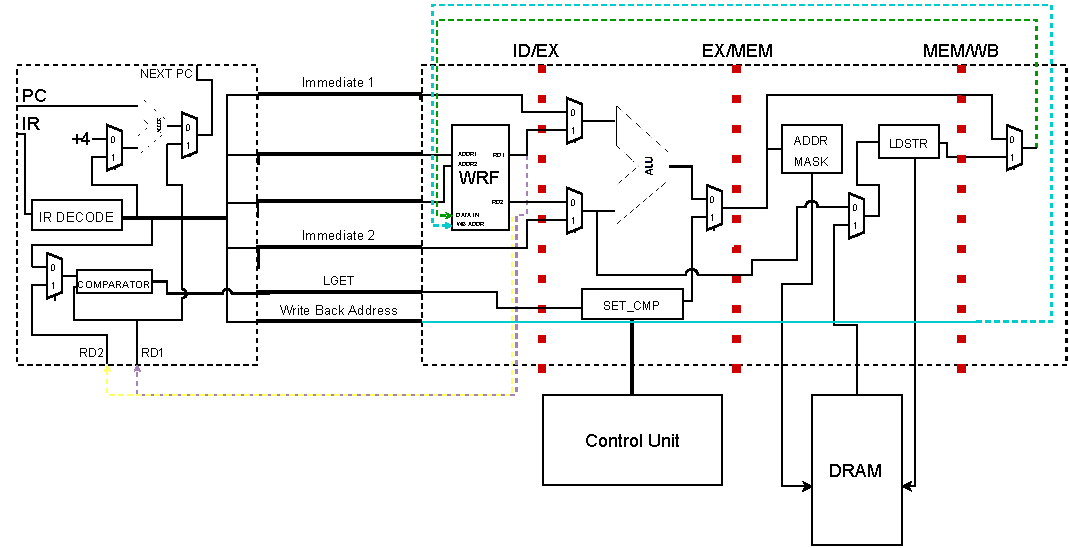
\includegraphics[width=0.91\textwidth]{chapters/2_dlx/images/DLX_DP.pdf}
    \caption{Schematic of the DLX Pipeline Structure}
    \label{DLX_DP}
\end{figure} 

As shown in figure \ref{DLX_DP}, the five pipeline stages are:

\begin{enumerate}
    \item \emph{Fetch}: not shown in the figure, it keeps track of the current instruction (IR) and the address of the next instruction to be fetched (PC).
    \item \emph{Decode}: it has the role of taking as input the current instruction (IR) and decoding it by extracting all the fields and dispatch them to the correct ports (Immediate 1, RS1, RS2, WB ADDR, Immediate 2). Furthermore, it's in charge of comparing values (from the Register File or an immediate) and computing the next PC given the actual PC. Last but not least, it keeps track of all the instructions in execution inside the pipeline and signals possible Data Hazard to the Control unit. By design choice, the Branch/Jump instructions are executed here instead of the Execute Stage, to lose only one clock cycle after a taken jump ideally (because of the wrong fetched instruction).
    \item \emph{Execute}: it takes the data from the Decode stage. Then, it does some computation on them, like adding them, multiply them, compute a shift and so on (refer to Table \ref{tab:alu_op} for available ALU operations), or outputs to the next stage the result of the comparison made in the Decode stage.
    \item \emph{Memory}: given the Address computed by the ALU during the previous stage and an optional Data, it's capable of doing a Load from the DRAM or a Store towards the DRAM. However, not all operations use this stage, so there is a bypass connection from the output of the EX stage towards the WB stage.
    \item \emph{Write Back}: the last stage of the pipeline selects the output from the ALU or the Memory (after a load operation) and gives it input to the Register File. Meanwhile, the destination address has been propagated through each stage and is now ready to be used by the Register File to store the final result. The Hazard Control Unit inside the Decode Stage intercepts this Write Back operation and knows that new instructions requiring this Data can now be executed.
\end{enumerate}


\section{Control Unit}

The Control Unit is one of the essential parts of the DLX processor. Its role is to orchestrate all the jobs through the processor's pipeline and manage dangerous situations.\\

Its interface is made of input signals (status signals from other components) and of control signals (towards other components), as described in Table \ref{table:cu:input_signals} and Table \ref{table:cu:output_signals}.

\begin{table}[H]
    \centering
    \begin{tabular}{l|l}
        \textbf{Signal Name} & \textbf{Description}\\
        \hline
        IR\_IN & Fetched Instruction, output from the IR Register \\
        HAZARD\_SIG & The Decode Stage is signaling a Hazard situation \\
        BUSY\_WINDOW & The Current RF Window has some registers in use \\
        SPILL & The Register File has started a push operations towards the memory \\
        FILL & The Register File has started a pop operations from the memory \\
        IRAM\_READY & The Instruction Memory has a data ready as output \\
        LGET & Comparison status from the comparator inside the Decode Unit\\
        DRAM\_READY & Indicates if the DRAM is ready or not\\
    \end{tabular}
    \caption{Input signals towards the Control Unit}
    \label{table:cu:input_signals}
\end{table}

\begin{table}[H]
    \centering
    \begin{tabular}{l|c|l}
        \textbf{Signal Name} & Sign & \textbf{Description}\\
        \hline
        PIPLIN\_IF\_EN & F & IF Stage enable: enable of IR register \\
        IF\_STALL & S & IF Stage stall: a NOP is insterted in the IR register \\
        PC\_EN & P & Enable of the PC register \\
        JUMP\_EN & J & JUMP must occur: Decode Stage will compute the new PC \\
        CALL & L & The Register File starts the context switch in a new window\\
        RET & E & The Register File must restore the previous window\\
        SEL\_CMPB & P & Reg or Imm field as comparator input in the Decode Stage\\
        UNSIGNED\_ID & U & All arithmetic units must consider operands as unsigned\\
        NPC\_SEL & N & Selects new PC (Adder or REG content)\\
        HAZARD\_TABLE\_WR1 & H & Enables log of the current instruction in the hazard control\\
        RF\_RD1\_EN & 1 & Enables the Read Port 1 in the RF\\
        RF\_RD2\_EN & 2 & Enables the Read Port 2 in the RF\\
        PIPLIN\_ID\_EN & D & ID Stage enable: enables all the ID pipeline REGs\\
        PIPLIN\_EX\_EN & X & EX Stage enable: enables all the EX pipeline REGs\\
        MUXA\_SEL & A & Input A of ALU: Immediate 1 or RD1\\
        MUXB\_SEL & B & Input B of ALU: Immediate 2 or RD2\\
        SEL\_ALU\_SETCMP & T & ALU or SET Comparator as EX stage output\\
        ALU\_OPCODE & \texttt{ALU} & ALU operation to be done\\
        SEL\_LGET & \texttt{SEL} & SET Comparator operation to be done\\
        DRAM\_WE & W & Enables the Write Operation in the DRAM\\
        DRAM\_RE & R & Enables the Read Operation in the DRAM\\
        DRAM\_ME & & Enable signal for the DRAM\\
        DATA\_SIZE & DS & Indicates the data of transfer towards/from the DRAM\\
        UNSIG\_SIGN\_N & U & Same as \emph{UNSIGNED\_ID} but 2 clock cycles delayed\\
        PIPLIN\_MEM\_EN & M & MEM Stage enable: enables all the MEM pipeline REGs\\
        WB\_MUX\_SEL & C & Selects MEM output or ALU out as content to write back\\
        PIPLIN\_WB\_EN & K & WB Stage enable: enables the Write signal in the RF\\
    \end{tabular}
    \caption{Output signals towards the Control Unit}
    \label{table:cu:output_signals}
\end{table}


\subsection{Control Words}

Going deeper into the Control Unit, it's possible to look at the generated Control Words for each Instruction. Each bit is referred to a Control Signal as indicated in Table \ref{table:cu:output_signals}, \emph{Sign} column, while a blank bit means that it's randomly assigned.

\begin{figure}[ht]
    \begin{center}
        \begin{bytefield}[endianness=big,bitwidth=0.03\linewidth]{32}
        \bitheader{0-31} \\
            \bitbox{1}{F} & \bitbox{1}{S} & \bitbox{1}{P} & \bitbox{1}{J} & \bitbox{1}{L} & \bitbox{1}{E} & \bitbox{1}{1} & \bitbox{1}{2} & \bitbox{1}{P} & \bitbox{1}{U} & \bitbox{1}{N} & \bitbox{1}{H} & \bitbox{1}{D} & \bitbox{1}{X} & \bitbox{1}{A} & \bitbox{1}{B} & \bitbox{5}{ALU} & \bitbox{3}{SEL} & \bitbox{1}{T} & \bitbox{1}{W} & \bitbox{1}{R} & \bitbox{2}{DS} & \bitbox{1}{M} & \bitbox{1}{C} & \bitbox{1}{K}
        \end{bytefield}
    \end{center}
    \caption{Control Word bits organization}
\end{figure}


\begin{figure}[H]
    \begin{center}
        \begin{bytefield}[endianness=big,bitwidth=0.0278\linewidth]{32}
        \bitheader{0-10, 11, 15, 16-31} \\

        \begin{rightwordgroup}{RTYPE}
            \bitbox{1}{1} & \bitbox{1}{0} & \bitbox{1}{1} & \bitbox{1}{0} & \bitbox{1}{0} & \bitbox{1}{0} & \bitbox{1}{1} & \bitbox{1}{1} & \bitbox{1}{1} & \bitbox{1}{0} & \bitbox{1}{0} & \bitbox{1}{1} & \bitbox{1}{1} & \bitbox{1}{1} & \bitbox{1}{0} & \bitbox{1}{0} & \bitbox{5}{} & \bitbox{3}{} & \bitbox{1}{0} & \bitbox{1}{0} & \bitbox{1}{0} & \bitbox{2}{00} & \bitbox{1}{1} & \bitbox{1}{0} & \bitbox{1}{1}
        \end{rightwordgroup}\\

        \begin{rightwordgroup}{J}
            \bitbox{1}{1} & \bitbox{1}{1} & \bitbox{1}{1} & \bitbox{1}{1} & \bitbox{1}{0} & \bitbox{1}{0} & \bitbox{1}{0} & \bitbox{1}{0} & \bitbox{1}{1} & \bitbox{1}{0} & \bitbox{1}{0} & \bitbox{1}{0} & \bitbox{1}{0} & \bitbox{1}{0} & \bitbox{1}{0} & \bitbox{1}{0} & \bitbox{5}{ADD} & \bitbox{3}{SEQ} & \bitbox{1}{0} & \bitbox{1}{0} & \bitbox{1}{0} & \bitbox{2}{00} & \bitbox{1}{0} & \bitbox{1}{0} & \bitbox{1}{0}
        \end{rightwordgroup}\\

        \begin{rightwordgroup}{JAL}
            \bitbox{1}{1} & \bitbox{1}{1} & \bitbox{1}{1} & \bitbox{1}{1} & \bitbox{1}{0} & \bitbox{1}{0} & \bitbox{1}{1} & \bitbox{1}{0} & \bitbox{1}{1} & \bitbox{1}{0} & \bitbox{1}{0} & \bitbox{1}{1} & \bitbox{1}{1} & \bitbox{1}{1} & \bitbox{1}{0} & \bitbox{1}{1} & \bitbox{5}{ADD} & \bitbox{3}{SEQ} & \bitbox{1}{0} & \bitbox{1}{0} & \bitbox{1}{0} & \bitbox{2}{00} & \bitbox{1}{1} & \bitbox{1}{0} & \bitbox{1}{1}
        \end{rightwordgroup}\\


        \end{bytefield}
    \end{center}
    \caption{Control Word for each instruction}
\end{figure}


\begin{figure}[H]
    \begin{center}
        \begin{bytefield}[endianness=big,bitwidth=0.0278\linewidth]{32}
        \bitheader{0-10, 11, 15, 16-31} \\

        \begin{rightwordgroup}{BEQZ}
            \bitbox{1}{1} & \bitbox{1}{0} & \bitbox{1}{1} & \bitbox{1}{ } & \bitbox{1}{0} & \bitbox{1}{0} & \bitbox{1}{1} & \bitbox{1}{1} & \bitbox{1}{1} & \bitbox{1}{0} & \bitbox{1}{0} & \bitbox{1}{0} & \bitbox{1}{0} & \bitbox{1}{0} & \bitbox{1}{0} & \bitbox{1}{0} & \bitbox{5}{ADD} & \bitbox{3}{SEQ} & \bitbox{1}{0} & \bitbox{1}{0} & \bitbox{1}{0} & \bitbox{2}{00} & \bitbox{1}{0} & \bitbox{1}{0} & \bitbox{1}{0}
        \end{rightwordgroup}\\

        \begin{rightwordgroup}{BNEZ}
            \bitbox{1}{1} & \bitbox{1}{0} & \bitbox{1}{1} & \bitbox{1}{ } & \bitbox{1}{0} & \bitbox{1}{0} & \bitbox{1}{1} & \bitbox{1}{1} & \bitbox{1}{1} & \bitbox{1}{0} & \bitbox{1}{0} & \bitbox{1}{0} & \bitbox{1}{0} & \bitbox{1}{0} & \bitbox{1}{0} & \bitbox{1}{0} & \bitbox{5}{ADD} & \bitbox{3}{SEQ} & \bitbox{1}{0} & \bitbox{1}{0} & \bitbox{1}{0} & \bitbox{2}{00} & \bitbox{1}{0} & \bitbox{1}{0} & \bitbox{1}{0}
        \end{rightwordgroup}\\

        \begin{rightwordgroup}{ADDI}
            \bitbox{1}{1} & \bitbox{1}{0} & \bitbox{1}{1} & \bitbox{1}{0} & \bitbox{1}{0} & \bitbox{1}{0} & \bitbox{1}{1} & \bitbox{1}{0} & \bitbox{1}{0} & \bitbox{1}{0} & \bitbox{1}{0} & \bitbox{1}{1} & \bitbox{1}{1} & \bitbox{1}{1} & \bitbox{1}{0} & \bitbox{1}{1} & \bitbox{5}{ADD} & \bitbox{3}{SEQ} & \bitbox{1}{0} & \bitbox{1}{0} & \bitbox{1}{0} & \bitbox{2}{00} & \bitbox{1}{1} & \bitbox{1}{0} & \bitbox{1}{1}
        \end{rightwordgroup}\\

        \begin{rightwordgroup}{ADDUI}
            \bitbox{1}{1} & \bitbox{1}{0} & \bitbox{1}{1} & \bitbox{1}{0} & \bitbox{1}{0} & \bitbox{1}{0} & \bitbox{1}{1} & \bitbox{1}{0} & \bitbox{1}{0} & \bitbox{1}{1} & \bitbox{1}{0} & \bitbox{1}{1} & \bitbox{1}{1} & \bitbox{1}{1} & \bitbox{1}{0} & \bitbox{1}{1} & \bitbox{5}{ADD} & \bitbox{3}{SEQ} & \bitbox{1}{0} & \bitbox{1}{0} & \bitbox{1}{0} & \bitbox{2}{00} & \bitbox{1}{1} & \bitbox{1}{0} & \bitbox{1}{1}
        \end{rightwordgroup}\\

        \begin{rightwordgroup}{SUBI}
            \bitbox{1}{1} & \bitbox{1}{0} & \bitbox{1}{1} & \bitbox{1}{0} & \bitbox{1}{0} & \bitbox{1}{0} & \bitbox{1}{1} & \bitbox{1}{0} & \bitbox{1}{0} & \bitbox{1}{0} & \bitbox{1}{0} & \bitbox{1}{1} & \bitbox{1}{1} & \bitbox{1}{1} & \bitbox{1}{0} & \bitbox{1}{1} & \bitbox{5}{SUB} & \bitbox{3}{SEQ} & \bitbox{1}{0} & \bitbox{1}{0} & \bitbox{1}{0} & \bitbox{2}{00} & \bitbox{1}{1} & \bitbox{1}{0} & \bitbox{1}{1}
        \end{rightwordgroup}\\

        \begin{rightwordgroup}{SUBUI}
            \bitbox{1}{1} & \bitbox{1}{0} & \bitbox{1}{1} & \bitbox{1}{0} & \bitbox{1}{0} & \bitbox{1}{0} & \bitbox{1}{1} & \bitbox{1}{0} & \bitbox{1}{0} & \bitbox{1}{1} & \bitbox{1}{0} & \bitbox{1}{1} & \bitbox{1}{1} & \bitbox{1}{1} & \bitbox{1}{0} & \bitbox{1}{1} & \bitbox{5}{SUB} & \bitbox{3}{SEQ} & \bitbox{1}{0} & \bitbox{1}{0} & \bitbox{1}{0} & \bitbox{2}{00} & \bitbox{1}{1} & \bitbox{1}{0} & \bitbox{1}{1}
        \end{rightwordgroup}\\

        \begin{rightwordgroup}{ANDI}
            \bitbox{1}{1} & \bitbox{1}{0} & \bitbox{1}{1} & \bitbox{1}{0} & \bitbox{1}{0} & \bitbox{1}{0} & \bitbox{1}{1} & \bitbox{1}{0} & \bitbox{1}{0} & \bitbox{1}{1} & \bitbox{1}{0} & \bitbox{1}{1} & \bitbox{1}{1} & \bitbox{1}{1} & \bitbox{1}{0} & \bitbox{1}{1} & \bitbox{5}{AND} & \bitbox{3}{SEQ} & \bitbox{1}{0} & \bitbox{1}{0} & \bitbox{1}{0} & \bitbox{2}{00} & \bitbox{1}{1} & \bitbox{1}{0} & \bitbox{1}{1}
        \end{rightwordgroup}\\

        \begin{rightwordgroup}{ORI}
            \bitbox{1}{1} & \bitbox{1}{0} & \bitbox{1}{1} & \bitbox{1}{0} & \bitbox{1}{0} & \bitbox{1}{0} & \bitbox{1}{1} & \bitbox{1}{0} & \bitbox{1}{0} & \bitbox{1}{1} & \bitbox{1}{0} & \bitbox{1}{1} & \bitbox{1}{1} & \bitbox{1}{1} & \bitbox{1}{0} & \bitbox{1}{1} & \bitbox{5}{OR} & \bitbox{3}{SEQ} & \bitbox{1}{0} & \bitbox{1}{0} & \bitbox{1}{0} & \bitbox{2}{00} & \bitbox{1}{1} & \bitbox{1}{0} & \bitbox{1}{1}
        \end{rightwordgroup}\\

        \begin{rightwordgroup}{XORI}
            \bitbox{1}{1} & \bitbox{1}{0} & \bitbox{1}{1} & \bitbox{1}{0} & \bitbox{1}{0} & \bitbox{1}{0} & \bitbox{1}{1} & \bitbox{1}{0} & \bitbox{1}{0} & \bitbox{1}{1} & \bitbox{1}{0} & \bitbox{1}{1} & \bitbox{1}{1} & \bitbox{1}{1} & \bitbox{1}{0} & \bitbox{1}{1} & \bitbox{5}{XOR} & \bitbox{3}{SEQ} & \bitbox{1}{0} & \bitbox{1}{0} & \bitbox{1}{0} & \bitbox{2}{00} & \bitbox{1}{1} & \bitbox{1}{0} & \bitbox{1}{1}
        \end{rightwordgroup}\\

        \begin{rightwordgroup}{LHI}
            \bitbox{1}{1} & \bitbox{1}{0} & \bitbox{1}{1} & \bitbox{1}{0} & \bitbox{1}{0} & \bitbox{1}{0} & \bitbox{1}{0} & \bitbox{1}{0} & \bitbox{1}{0} & \bitbox{1}{0} & \bitbox{1}{0} & \bitbox{1}{1} & \bitbox{1}{1} & \bitbox{1}{1} & \bitbox{1}{1} & \bitbox{1}{1} & \bitbox{5}{SLL} & \bitbox{3}{SEQ} & \bitbox{1}{0} & \bitbox{1}{0} & \bitbox{1}{0} & \bitbox{2}{00} & \bitbox{1}{1} & \bitbox{1}{0} & \bitbox{1}{1}
        \end{rightwordgroup}\\

        \begin{rightwordgroup}{JR}
            \bitbox{1}{1} & \bitbox{1}{1} & \bitbox{1}{1} & \bitbox{1}{1} & \bitbox{1}{0} & \bitbox{1}{0} & \bitbox{1}{1} & \bitbox{1}{0} & \bitbox{1}{1} & \bitbox{1}{0} & \bitbox{1}{1} & \bitbox{1}{0} & \bitbox{1}{0} & \bitbox{1}{0} & \bitbox{1}{0} & \bitbox{1}{0} & \bitbox{5}{ADD} & \bitbox{3}{SEQ} & \bitbox{1}{0} & \bitbox{1}{0} & \bitbox{1}{0} & \bitbox{2}{00} & \bitbox{1}{0} & \bitbox{1}{0} & \bitbox{1}{0}
        \end{rightwordgroup}\\

        \begin{rightwordgroup}{JALR}
            \bitbox{1}{1} & \bitbox{1}{1} & \bitbox{1}{1} & \bitbox{1}{1} & \bitbox{1}{0} & \bitbox{1}{0} & \bitbox{1}{1} & \bitbox{1}{1} & \bitbox{1}{1} & \bitbox{1}{0} & \bitbox{1}{1} & \bitbox{1}{1} & \bitbox{1}{1} & \bitbox{1}{1} & \bitbox{1}{0} & \bitbox{1}{1} & \bitbox{5}{ADD} & \bitbox{3}{SEQ} & \bitbox{1}{0} & \bitbox{1}{0} & \bitbox{1}{0} & \bitbox{2}{00} & \bitbox{1}{1} & \bitbox{1}{0} & \bitbox{1}{1}
        \end{rightwordgroup}\\

        \begin{rightwordgroup}{SLLI}
            \bitbox{1}{1} & \bitbox{1}{0} & \bitbox{1}{1} & \bitbox{1}{0} & \bitbox{1}{0} & \bitbox{1}{0} & \bitbox{1}{1} & \bitbox{1}{0} & \bitbox{1}{0} & \bitbox{1}{1} & \bitbox{1}{0} & \bitbox{1}{1} & \bitbox{1}{1} & \bitbox{1}{1} & \bitbox{1}{0} & \bitbox{1}{1} & \bitbox{5}{SLL} & \bitbox{3}{SEQ} & \bitbox{1}{0} & \bitbox{1}{0} & \bitbox{1}{0} & \bitbox{2}{00} & \bitbox{1}{1} & \bitbox{1}{0} & \bitbox{1}{1}
        \end{rightwordgroup}\\

        \begin{rightwordgroup}{NOP}
            \bitbox{1}{1} & \bitbox{1}{0} & \bitbox{1}{1} & \bitbox{1}{0} & \bitbox{1}{0} & \bitbox{1}{0} & \bitbox{1}{0} & \bitbox{1}{0} & \bitbox{1}{1} & \bitbox{1}{0} & \bitbox{1}{0} & \bitbox{1}{0} & \bitbox{1}{0} & \bitbox{1}{0} & \bitbox{1}{0} & \bitbox{1}{0} & \bitbox{5}{ADD} & \bitbox{3}{SEQ} & \bitbox{1}{0} & \bitbox{1}{0} & \bitbox{1}{0} & \bitbox{2}{00} & \bitbox{1}{0} & \bitbox{1}{0} & \bitbox{1}{0}
        \end{rightwordgroup}\\

        \begin{rightwordgroup}{SRLI}
            \bitbox{1}{1} & \bitbox{1}{0} & \bitbox{1}{1} & \bitbox{1}{0} & \bitbox{1}{0} & \bitbox{1}{0} & \bitbox{1}{1} & \bitbox{1}{0} & \bitbox{1}{0} & \bitbox{1}{1} & \bitbox{1}{0} & \bitbox{1}{1} & \bitbox{1}{1} & \bitbox{1}{1} & \bitbox{1}{0} & \bitbox{1}{1} & \bitbox{5}{SRL} & \bitbox{3}{SEQ} & \bitbox{1}{0} & \bitbox{1}{0} & \bitbox{1}{0} & \bitbox{2}{00} & \bitbox{1}{1} & \bitbox{1}{0} & \bitbox{1}{1}
        \end{rightwordgroup}\\

        \begin{rightwordgroup}{SRAI}
            \bitbox{1}{1} & \bitbox{1}{0} & \bitbox{1}{1} & \bitbox{1}{0} & \bitbox{1}{0} & \bitbox{1}{0} & \bitbox{1}{1} & \bitbox{1}{0} & \bitbox{1}{1} & \bitbox{1}{1} & \bitbox{1}{0} & \bitbox{1}{1} & \bitbox{1}{1} & \bitbox{1}{1} & \bitbox{1}{0} & \bitbox{1}{1} & \bitbox{5}{SRA} & \bitbox{3}{SEQ} & \bitbox{1}{0} & \bitbox{1}{0} & \bitbox{1}{0} & \bitbox{2}{00} & \bitbox{1}{1} & \bitbox{1}{0} & \bitbox{1}{1}
        \end{rightwordgroup}\\

        \begin{rightwordgroup}{SEQI}
            \bitbox{1}{1} & \bitbox{1}{0} & \bitbox{1}{1} & \bitbox{1}{0} & \bitbox{1}{0} & \bitbox{1}{0} & \bitbox{1}{1} & \bitbox{1}{0} & \bitbox{1}{0} & \bitbox{1}{0} & \bitbox{1}{0} & \bitbox{1}{1} & \bitbox{1}{1} & \bitbox{1}{1} & \bitbox{1}{0} & \bitbox{1}{1} & \bitbox{5}{ADD} & \bitbox{3}{SEQ} & \bitbox{1}{1} & \bitbox{1}{0} & \bitbox{1}{0} & \bitbox{2}{00} & \bitbox{1}{1} & \bitbox{1}{0} & \bitbox{1}{1}
        \end{rightwordgroup}\\

        \begin{rightwordgroup}{SNEI}
            \bitbox{1}{1} & \bitbox{1}{0} & \bitbox{1}{1} & \bitbox{1}{0} & \bitbox{1}{0} & \bitbox{1}{0} & \bitbox{1}{1} & \bitbox{1}{0} & \bitbox{1}{0} & \bitbox{1}{0} & \bitbox{1}{0} & \bitbox{1}{1} & \bitbox{1}{1} & \bitbox{1}{1} & \bitbox{1}{0} & \bitbox{1}{1} & \bitbox{5}{ADD} & \bitbox{3}{SNE} & \bitbox{1}{1} & \bitbox{1}{0} & \bitbox{1}{0} & \bitbox{2}{00} & \bitbox{1}{1} & \bitbox{1}{0} & \bitbox{1}{1}
        \end{rightwordgroup}\\

        \begin{rightwordgroup}{SLTI}
            \bitbox{1}{1} & \bitbox{1}{0} & \bitbox{1}{1} & \bitbox{1}{0} & \bitbox{1}{0} & \bitbox{1}{0} & \bitbox{1}{1} & \bitbox{1}{0} & \bitbox{1}{0} & \bitbox{1}{0} & \bitbox{1}{0} & \bitbox{1}{1} & \bitbox{1}{1} & \bitbox{1}{1} & \bitbox{1}{0} & \bitbox{1}{1} & \bitbox{5}{ADD} & \bitbox{3}{SLT} & \bitbox{1}{1} & \bitbox{1}{0} & \bitbox{1}{0} & \bitbox{2}{00} & \bitbox{1}{1} & \bitbox{1}{0} & \bitbox{1}{1}
        \end{rightwordgroup}\\

        \begin{rightwordgroup}{SGTI}
                \bitbox{1}{1} & \bitbox{1}{0} & \bitbox{1}{1} & \bitbox{1}{0} & \bitbox{1}{0} & \bitbox{1}{0} & \bitbox{1}{1} & \bitbox{1}{0} & \bitbox{1}{0} & \bitbox{1}{0} & \bitbox{1}{0} & \bitbox{1}{1} & \bitbox{1}{1} & \bitbox{1}{1} & \bitbox{1}{0} & \bitbox{1}{1} & \bitbox{5}{ADD} & \bitbox{3}{SGT} & \bitbox{1}{1} & \bitbox{1}{0} & \bitbox{1}{0} & \bitbox{2}{00} & \bitbox{1}{1} & \bitbox{1}{0} & \bitbox{1}{1}
        \end{rightwordgroup}\\

        \begin{rightwordgroup}{SLEI}
            \bitbox{1}{1} & \bitbox{1}{0} & \bitbox{1}{1} & \bitbox{1}{0} & \bitbox{1}{0} & \bitbox{1}{0} & \bitbox{1}{1} & \bitbox{1}{0} & \bitbox{1}{0} & \bitbox{1}{0} & \bitbox{1}{0} & \bitbox{1}{1} & \bitbox{1}{1} & \bitbox{1}{1} & \bitbox{1}{0} & \bitbox{1}{1} & \bitbox{5}{ADD} & \bitbox{3}{SLE} & \bitbox{1}{1} & \bitbox{1}{0} & \bitbox{1}{0} & \bitbox{2}{00} & \bitbox{1}{1} & \bitbox{1}{0} & \bitbox{1}{1}
        \end{rightwordgroup}\\

        \begin{rightwordgroup}{SGEI}
            \bitbox{1}{1} & \bitbox{1}{0} & \bitbox{1}{1} & \bitbox{1}{0} & \bitbox{1}{0} & \bitbox{1}{0} & \bitbox{1}{1} & \bitbox{1}{0} & \bitbox{1}{0} & \bitbox{1}{0} & \bitbox{1}{0} & \bitbox{1}{1} & \bitbox{1}{1} & \bitbox{1}{1} & \bitbox{1}{0} & \bitbox{1}{1} & \bitbox{5}{ADD} & \bitbox{3}{SGE} & \bitbox{1}{1} & \bitbox{1}{0} & \bitbox{1}{0} & \bitbox{2}{00} & \bitbox{1}{1} & \bitbox{1}{0} & \bitbox{1}{1}
        \end{rightwordgroup}\\

        \begin{rightwordgroup}{CALL}
            \bitbox{1}{1} & \bitbox{1}{1} & \bitbox{1}{1} & \bitbox{1}{1} & \bitbox{1}{0} & \bitbox{1}{0} & \bitbox{1}{1} & \bitbox{1}{0} & \bitbox{1}{1} & \bitbox{1}{0} & \bitbox{1}{0} & \bitbox{1}{1} & \bitbox{1}{1} & \bitbox{1}{1} & \bitbox{1}{0} & \bitbox{1}{1} & \bitbox{5}{ADD} & \bitbox{3}{SEQ} & \bitbox{1}{0} & \bitbox{1}{0} & \bitbox{1}{0} & \bitbox{2}{00} & \bitbox{1}{1} & \bitbox{1}{0} & \bitbox{1}{1}
        \end{rightwordgroup}\\

        \begin{rightwordgroup}{RET}
            \bitbox{1}{1} & \bitbox{1}{1} & \bitbox{1}{1} & \bitbox{1}{1} & \bitbox{1}{0} & \bitbox{1}{1} & \bitbox{1}{1} & \bitbox{1}{0} & \bitbox{1}{0} & \bitbox{1}{0} & \bitbox{1}{1} & \bitbox{1}{0} & \bitbox{1}{0} & \bitbox{1}{0} & \bitbox{1}{0} & \bitbox{1}{0} & \bitbox{5}{ADD} & \bitbox{3}{SEQ} & \bitbox{1}{0} & \bitbox{1}{0} & \bitbox{1}{0} & \bitbox{2}{00} & \bitbox{1}{0} & \bitbox{1}{0} & \bitbox{1}{0}
        \end{rightwordgroup}\\

        \begin{rightwordgroup}{LB}
            \bitbox{1}{1} & \bitbox{1}{0} & \bitbox{1}{1} & \bitbox{1}{0} & \bitbox{1}{0} & \bitbox{1}{0} & \bitbox{1}{1} & \bitbox{1}{0} & \bitbox{1}{0} & \bitbox{1}{0} & \bitbox{1}{0} & \bitbox{1}{1} & \bitbox{1}{1} & \bitbox{1}{1} & \bitbox{1}{0} & \bitbox{1}{1} & \bitbox{5}{ADD} & \bitbox{3}{SEQ} & \bitbox{1}{0} & \bitbox{1}{0} & \bitbox{1}{1} & \bitbox{2}{10} & \bitbox{1}{1} & \bitbox{1}{1} & \bitbox{1}{1}
        \end{rightwordgroup}\\

        \begin{rightwordgroup}{LH}
            \bitbox{1}{1} & \bitbox{1}{0} & \bitbox{1}{1} & \bitbox{1}{0} & \bitbox{1}{0} & \bitbox{1}{0} & \bitbox{1}{1} & \bitbox{1}{0} & \bitbox{1}{0} & \bitbox{1}{0} & \bitbox{1}{0} & \bitbox{1}{1} & \bitbox{1}{1} & \bitbox{1}{1} & \bitbox{1}{0} & \bitbox{1}{1} & \bitbox{5}{ADD} & \bitbox{3}{SEQ} & \bitbox{1}{0} & \bitbox{1}{0} & \bitbox{1}{1} & \bitbox{2}{01} & \bitbox{1}{1} & \bitbox{1}{1} & \bitbox{1}{1}
        \end{rightwordgroup}\\

        \begin{rightwordgroup}{LW}
            \bitbox{1}{1} & \bitbox{1}{0} & \bitbox{1}{1} & \bitbox{1}{0} & \bitbox{1}{0} & \bitbox{1}{0} & \bitbox{1}{1} & \bitbox{1}{0} & \bitbox{1}{0} & \bitbox{1}{0} & \bitbox{1}{0} & \bitbox{1}{1} & \bitbox{1}{1} & \bitbox{1}{1} & \bitbox{1}{0} & \bitbox{1}{1} & \bitbox{5}{ADD} & \bitbox{3}{SEQ} & \bitbox{1}{0} & \bitbox{1}{0} & \bitbox{1}{1} & \bitbox{2}{00} & \bitbox{1}{1} & \bitbox{1}{1} & \bitbox{1}{1}
        \end{rightwordgroup}\\

        \begin{rightwordgroup}{LBU}
            \bitbox{1}{1} & \bitbox{1}{0} & \bitbox{1}{1} & \bitbox{1}{0} & \bitbox{1}{0} & \bitbox{1}{0} & \bitbox{1}{1} & \bitbox{1}{0} & \bitbox{1}{0} & \bitbox{1}{1} & \bitbox{1}{0} & \bitbox{1}{1} & \bitbox{1}{1} & \bitbox{1}{1} & \bitbox{1}{0} & \bitbox{1}{1} & \bitbox{5}{ADD} & \bitbox{3}{SEQ} & \bitbox{1}{0} & \bitbox{1}{0} & \bitbox{1}{1} & \bitbox{2}{10} & \bitbox{1}{1} & \bitbox{1}{1} & \bitbox{1}{1}
        \end{rightwordgroup}\\

        \begin{rightwordgroup}{LHU}
            \bitbox{1}{1} & \bitbox{1}{0} & \bitbox{1}{1} & \bitbox{1}{0} & \bitbox{1}{0} & \bitbox{1}{0} & \bitbox{1}{1} & \bitbox{1}{0} & \bitbox{1}{0} & \bitbox{1}{1} & \bitbox{1}{0} & \bitbox{1}{1} & \bitbox{1}{1} & \bitbox{1}{1} & \bitbox{1}{0} & \bitbox{1}{1} & \bitbox{5}{ADD} & \bitbox{3}{SEQ} & \bitbox{1}{0} & \bitbox{1}{0} & \bitbox{1}{1} & \bitbox{2}{01} & \bitbox{1}{1} & \bitbox{1}{1} & \bitbox{1}{1}
        \end{rightwordgroup}\\

        \begin{rightwordgroup}{SB}
            \bitbox{1}{1} & \bitbox{1}{0} & \bitbox{1}{1} & \bitbox{1}{0} & \bitbox{1}{0} & \bitbox{1}{0} & \bitbox{1}{1} & \bitbox{1}{1} & \bitbox{1}{0} & \bitbox{1}{0} & \bitbox{1}{0} & \bitbox{1}{0} & \bitbox{1}{1} & \bitbox{1}{1} & \bitbox{1}{0} & \bitbox{1}{1} & \bitbox{5}{ADD} & \bitbox{3}{SEQ} & \bitbox{1}{0} & \bitbox{1}{1} & \bitbox{1}{0} & \bitbox{2}{10} & \bitbox{1}{1} & \bitbox{1}{0} & \bitbox{1}{0}
        \end{rightwordgroup}\\

        \begin{rightwordgroup}{SH}
            \bitbox{1}{1} & \bitbox{1}{0} & \bitbox{1}{1} & \bitbox{1}{0} & \bitbox{1}{0} & \bitbox{1}{0} & \bitbox{1}{1} & \bitbox{1}{1} & \bitbox{1}{0} & \bitbox{1}{0} & \bitbox{1}{0} & \bitbox{1}{0} & \bitbox{1}{1} & \bitbox{1}{1} & \bitbox{1}{0} & \bitbox{1}{1} & \bitbox{5}{ADD} & \bitbox{3}{SEQ} & \bitbox{1}{0} & \bitbox{1}{1} & \bitbox{1}{0} & \bitbox{2}{01} & \bitbox{1}{1} & \bitbox{1}{0} & \bitbox{1}{0}
        \end{rightwordgroup}\\

        \begin{rightwordgroup}{SW}
            \bitbox{1}{1} & \bitbox{1}{0} & \bitbox{1}{1} & \bitbox{1}{0} & \bitbox{1}{0} & \bitbox{1}{0} & \bitbox{1}{1} & \bitbox{1}{1} & \bitbox{1}{0} & \bitbox{1}{0} & \bitbox{1}{0} & \bitbox{1}{0} & \bitbox{1}{1} & \bitbox{1}{1} & \bitbox{1}{0} & \bitbox{1}{1} & \bitbox{5}{ADD} & \bitbox{3}{SEQ} & \bitbox{1}{0} & \bitbox{1}{1} & \bitbox{1}{0} & \bitbox{2}{00} & \bitbox{1}{1} & \bitbox{1}{0} & \bitbox{1}{0}
        \end{rightwordgroup}\\


        \begin{rightwordgroup}{TKTM}
            \bitbox{1}{1} & \bitbox{1}{0} & \bitbox{1}{1} & \bitbox{1}{0} & \bitbox{1}{0} & \bitbox{1}{0} & \bitbox{1}{1} & \bitbox{1}{0} & \bitbox{1}{1} & \bitbox{1}{0} & \bitbox{1}{0} & \bitbox{1}{1} & \bitbox{1}{1} & \bitbox{1}{1} & \bitbox{1}{0} & \bitbox{1}{1} & \bitbox{5}{ADD} & \bitbox{3}{SEQ} & \bitbox{1}{0} & \bitbox{1}{0} & \bitbox{1}{0} & \bitbox{2}{00} & \bitbox{1}{1} & \bitbox{1}{0} & \bitbox{1}{1}
        \end{rightwordgroup}\\

        \begin{rightwordgroup}{SLTUI}
            \bitbox{1}{1} & \bitbox{1}{0} & \bitbox{1}{1} & \bitbox{1}{0} & \bitbox{1}{0} & \bitbox{1}{0} & \bitbox{1}{1} & \bitbox{1}{0} & \bitbox{1}{0} & \bitbox{1}{1} & \bitbox{1}{0} & \bitbox{1}{1} & \bitbox{1}{1} & \bitbox{1}{1} & \bitbox{1}{0} & \bitbox{1}{1} & \bitbox{5}{ADD} & \bitbox{3}{SLT} & \bitbox{1}{1} & \bitbox{1}{0} & \bitbox{1}{0} & \bitbox{2}{00} & \bitbox{1}{1} & \bitbox{1}{0} & \bitbox{1}{1}
        \end{rightwordgroup}\\

        \begin{rightwordgroup}{SGTUI}
            \bitbox{1}{1} & \bitbox{1}{0} & \bitbox{1}{1} & \bitbox{1}{0} & \bitbox{1}{0} & \bitbox{1}{0} & \bitbox{1}{1} & \bitbox{1}{0} & \bitbox{1}{0} & \bitbox{1}{1} & \bitbox{1}{0} & \bitbox{1}{1} & \bitbox{1}{1} & \bitbox{1}{1} & \bitbox{1}{0} & \bitbox{1}{1} & \bitbox{5}{ADD} & \bitbox{3}{SGT} & \bitbox{1}{1} & \bitbox{1}{0} & \bitbox{1}{0} & \bitbox{2}{00} & \bitbox{1}{1} & \bitbox{1}{0} & \bitbox{1}{1}
        \end{rightwordgroup}\\

        \begin{rightwordgroup}{SLEUI}
            \bitbox{1}{1} & \bitbox{1}{0} & \bitbox{1}{1} & \bitbox{1}{0} & \bitbox{1}{0} & \bitbox{1}{0} & \bitbox{1}{1} & \bitbox{1}{0} & \bitbox{1}{0} & \bitbox{1}{1} & \bitbox{1}{0} & \bitbox{1}{1} & \bitbox{1}{1} & \bitbox{1}{1} & \bitbox{1}{0} & \bitbox{1}{1} & \bitbox{5}{ADD} & \bitbox{3}{SLE} & \bitbox{1}{1} & \bitbox{1}{0} & \bitbox{1}{0} & \bitbox{2}{00} & \bitbox{1}{1} & \bitbox{1}{0} & \bitbox{1}{1}
        \end{rightwordgroup}\\

        \begin{rightwordgroup}{SGEUI}
            \bitbox{1}{1} & \bitbox{1}{0} & \bitbox{1}{1} & \bitbox{1}{0} & \bitbox{1}{0} & \bitbox{1}{0} & \bitbox{1}{1} & \bitbox{1}{0} & \bitbox{1}{0} & \bitbox{1}{1} & \bitbox{1}{0} & \bitbox{1}{1} & \bitbox{1}{1} & \bitbox{1}{1} & \bitbox{1}{0} & \bitbox{1}{1} & \bitbox{5}{ADD} & \bitbox{3}{SGE} & \bitbox{1}{1} & \bitbox{1}{0} & \bitbox{1}{0} & \bitbox{2}{00} & \bitbox{1}{1} & \bitbox{1}{0} & \bitbox{1}{1}
        \end{rightwordgroup}\\


        \begin{rightwordgroup}{BGT}
            \bitbox{1}{1} & \bitbox{1}{0} & \bitbox{1}{1} & \bitbox{1}{} & \bitbox{1}{0} & \bitbox{1}{0} & \bitbox{1}{1} & \bitbox{1}{1} & \bitbox{1}{1} & \bitbox{1}{0} & \bitbox{1}{0} & \bitbox{1}{0} & \bitbox{1}{0} & \bitbox{1}{0} & \bitbox{1}{0} & \bitbox{1}{0} & \bitbox{5}{ADD} & \bitbox{3}{SEQ} & \bitbox{1}{0} & \bitbox{1}{0} & \bitbox{1}{0} & \bitbox{2}{00} & \bitbox{1}{0} & \bitbox{1}{0} & \bitbox{1}{0}
        \end{rightwordgroup}\\

        \begin{rightwordgroup}{BGE}
            \bitbox{1}{1} & \bitbox{1}{0} & \bitbox{1}{1} & \bitbox{1}{} & \bitbox{1}{0} & \bitbox{1}{0} & \bitbox{1}{1} & \bitbox{1}{1} & \bitbox{1}{1} & \bitbox{1}{0} & \bitbox{1}{0} & \bitbox{1}{0} & \bitbox{1}{0} & \bitbox{1}{0} & \bitbox{1}{0} & \bitbox{1}{0} & \bitbox{5}{ADD} & \bitbox{3}{SEQ} & \bitbox{1}{0} & \bitbox{1}{0} & \bitbox{1}{0} & \bitbox{2}{00} & \bitbox{1}{0} & \bitbox{1}{0} & \bitbox{1}{0}
        \end{rightwordgroup}\\

        \begin{rightwordgroup}{BLT}
            \bitbox{1}{1} & \bitbox{1}{0} & \bitbox{1}{1} & \bitbox{1}{} & \bitbox{1}{0} & \bitbox{1}{0} & \bitbox{1}{1} & \bitbox{1}{1} & \bitbox{1}{1} & \bitbox{1}{0} & \bitbox{1}{0} & \bitbox{1}{0} & \bitbox{1}{0} & \bitbox{1}{0} & \bitbox{1}{0} & \bitbox{1}{0} & \bitbox{5}{ADD} & \bitbox{3}{SEQ} & \bitbox{1}{0} & \bitbox{1}{0} & \bitbox{1}{0} & \bitbox{2}{00} & \bitbox{1}{0} & \bitbox{1}{0} & \bitbox{1}{0}
        \end{rightwordgroup}\\

        \begin{rightwordgroup}{BLE}
            \bitbox{1}{1} & \bitbox{1}{0} & \bitbox{1}{1} & \bitbox{1}{} & \bitbox{1}{0} & \bitbox{1}{0} & \bitbox{1}{1} & \bitbox{1}{1} & \bitbox{1}{1} & \bitbox{1}{0} & \bitbox{1}{0} & \bitbox{1}{0} & \bitbox{1}{0} & \bitbox{1}{0} & \bitbox{1}{0} & \bitbox{1}{0} & \bitbox{5}{ADD} & \bitbox{3}{SEQ} & \bitbox{1}{0} & \bitbox{1}{0} & \bitbox{1}{0} & \bitbox{2}{00} & \bitbox{1}{0} & \bitbox{1}{0} & \bitbox{1}{0}
        \end{rightwordgroup}\\

        \end{bytefield}
    \end{center}
    \caption{Control Word for each instruction}
\end{figure}




\subsection{Internal organization of the Control Unit}

The Control Unit internally is organized mainly with a stage that converts the actual Instruction into a Control Word. Then this control word is propagated to support all the pipeline stages, as shown in Figure \ref{dlx:cu:schematic}.

\begin{figure}[H]
    \centering
    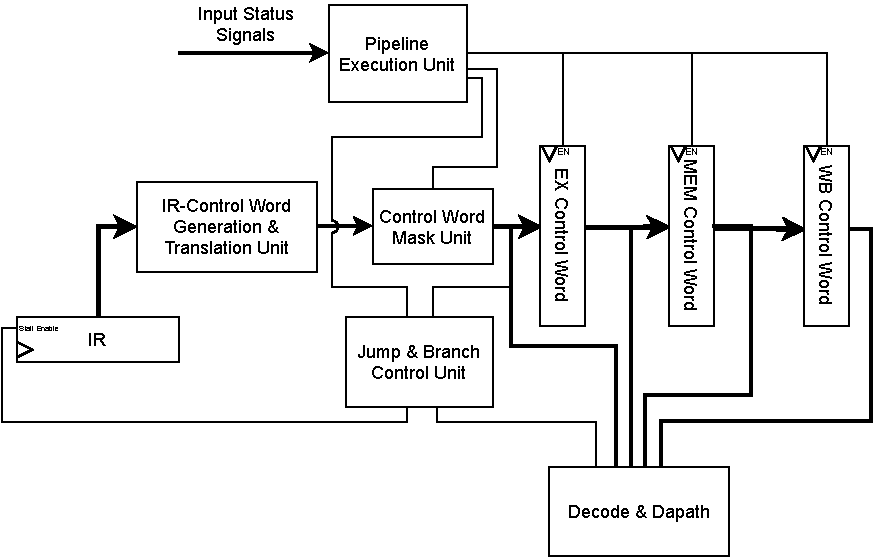
\includegraphics[width=0.72\textwidth]{chapters/2_dlx/images/DLX-Cu.pdf}
    \caption{Schematic of the DLX Control Unit}
    \label{dlx:cu:schematic}
\end{figure} 

It is made mainly by the following components:

\begin{itemize}
    \item IR-Control Word Generation \& Translation Unit: its role is to take the instruction given as input and output, a valid Control Word related to that instruction.
    \item Pipeline Execution Unit: it's in charge of controlling the Pipeline Flow and stop it in case of needs and/or masking the actual Control Word to prevent its propagation through the chain in case of Hazards.
    \item Control Word Mask Unit: when the \emph{Pipeline Execution Unit} signals to mask the control word, this unit will do it by disabling all the bits in the CW that referees to the stage enabling signals.
    \item Jump \& Branch Control unit: given the Control Word and other internal control signals, its job is to manage (by enabling or disabling them) signals like \emph{CALL}, \emph{RET}, \emph{JUMP\_EN} and \emph{IF\_STALL}.
\end{itemize}

% \begin{box_implementation_details}
%     {\large{\textbf{Implementation details: CW Generation Unit}}}
%   \newline
%     As said, the \emph{IR-Control Word Generation \& Translation Unit} is in charge of taking as input the actual instruction and to give as output a valid control word. How the mapping IR$\xrightarrow$CW is done?\\
% \end{box_implementation_details}


\section{Memory Interface}

The DLX processor has a Harvard architecture, with two 32-bit data buses carrying instructions and data respectively. Only load and store instructions can access data from Data Memory. The data are stored in memory in a Big-Endian format.\\

\begin{center}
    \begin{bytefield}[endianness=big,bitwidth=0.03\linewidth]{32}
    \bitheader{0, 7, 8, 15, 16, 23, 24, 31} \\
    \bitbox{32}{Word at address A}\\
    \bitbox{16}{Half at address A} & \bitbox{16}{Word at address A+2}\\
    \bitbox{8}{Byte at address A} & \bitbox{8}{Byte at address A+1} & \bitbox{8}{Byte at address A+2} & \bitbox{8}{Byte at address A+3}\\
    \end{bytefield}
\end{center}

The third RAM required, the one for the register file, is not under the User's direct access. It's managed as a Stack memory by the Register File for automatic subroutines management, and it has a dedicated interface. It can be merged with the Data Memory with external logic.\\

All the subsequent paragraphs are referred in the same way to all the three memory types.

\subsection{Signals and Timing}
The signals in the DLX processor bus interface can be grouped into tree categories:
\begin{itemize}
    \itemsep0sp
    \item Address class signals
    \item Memory Request signals
    \item Data class signals
\end{itemize}

The \emph{Address class signals} are:
\begin{itemize}
    \itemsep0sp
    \item A{[31:0]}
    \item DATA\_SIZE{[1:0]} \emph{or MAS{[1:0]}}
\end{itemize}

The \emph{Memory Request signals} are:
\begin{itemize}
    \itemsep0sp
    \item Enable
    \item $R\overline{W}$
    \item Ready
\end{itemize}

Moreover, all the memories connected must agree on a specific protocol both for writing and reading operations. The most important thing to take under consideration is the \emph{Ready} signal: it must be high only when the operation is completed. For example, after a data read, the \emph{Ready} stays at 1 only when the data is valid. If, meanwhile, the address changes, the \emph{Ready} signal must go off.

\begin{center}
    \begin{tikztimingtable}[%
        timing/dslope=0.2,
        timing/.style={x=8ex,y=2ex},
        x=8ex,
        timing/rowdist=3ex,
        timing/name/.style={font=\sffamily\scriptsize}
    ]
        \busref{CLK}                & 16{c} \\
        \busref[31:0]{Address}      & 2x 1D{$A_1$} 2D{$A_2$} 1X 1D{$A_4$} UX \\
        \busref[1:0]{MAS}           & 2x 1D{WORD 00} 2D{HALF 01} X 1D{BYTE 10} 2X\\
        \busref{Enable}             & 1L 2H HL HL L\\
        \busref{$R\overline{W}$}              & 1L 2H 2H LH L\\
        Ready                       & ll lh lh hh ll lh LL\\
        \busref[31:0]{Data In}      & 2x 2x 1X 1X 1X 1D{$D_1$} XX \\
        \busref[31:0]{DATA Out}      & 2x x1d{$D_1$} x3d{$D_2$} 4X  \\
        \extracode
        \begin{pgfonlayer}{background}
        \begin{scope}[semitransparent ,semithick]
        \vertlines[darkgray,dotted]{0.5,1.5 ,...,8.0}
        \end{scope}
        \end{pgfonlayer}
    \end{tikztimingtable}
\end{center}


If the Memory in use can't accomplish this timing, an external \emph{Memory Control Unit} must be placed between the CPU and the Memory.

\subsection{Memory Addressing}
A[31:0] is the 32-bit address bus that specifies the address for the transfer. All addresses are byte addresses, so a burst of word accesses results in the address bus incrementing by four for each cycle.\\

The address bus provides 4GB of linear addressing space, and this can be used externally in different manners, like in an SoC with memory-mapped peripherals that share the same address space.\\

When word access is signaled, the memory system ignores the bottom two bits, A[1:0], and when halfword access is signaled, the memory system ignores the bottom bit, A[0]. However, the core already masks the two LSBs when needed.

\subsection{Memory Data Size: the MAS[1:0] signal}
\label{mas}

The \emph{MAS[1:0]} bus encodes the size of the transfer. The DLX processor can transfer word, halfword, and byte quantities and the processor indicates the size of the transfer through this signal.\\

The \emph{MAS[1:0]} signal is supposed to be used in combination with \emph{A[1:0]} to know precisely which byte is taken under consideration during an operation.

\subsection{Memory Read}

When an half-word or byte read is performed, a 32-bit memory system can return the complete 32-bit word for simplicity, and the processor extracts the valid half-word or byte field from it as shown in Table \ref{table:memory_read_configuration}. Other byte lanes will be ignored. For 8 and 16 bit memories, the data must be placed on the right byte lanes in the data bus.

\begin{table}[H]
    \centering
    \begin{tabular}{|l|c|l|l|}
    \hline
        DATA\_SIZE[1:0] & A[1:0] & D[31:0] & DLX Register \\ \hline
        00 WORD & 00 & \texttt{0xAABBCCDD} & \texttt{0xAABBCCDD} \\ \hline
        01 HALF & 00 & \texttt{0xAABB----} & \texttt{0x0000AABB} \\ \hline
        01 HALF & 10 & \texttt{0x----CCDD} & \texttt{0x0000CCDD} \\ \hline
        10 BYTE & 00 & \texttt{0xAA------} & \texttt{0x000000AA} \\ \hline
        10 BYTE & 01 & \texttt{0x--BB----} & \texttt{0x000000BB} \\ \hline
        10 BYTE & 10 & \texttt{0x----CC--} & \texttt{0x000000CC} \\ \hline
        10 BYTE & 11 & \texttt{0x------DD} & \texttt{0x000000DD} \\ \hline
    \end{tabular}
    \caption{How data are read by the CPU in different MAS configurations}
    \label{table:memory_read_configuration}
\end{table}

\subsection{Memory Write}

Instead, when the DLX processor performs a byte or half-word write, the data being written is replicated across the data bus, as shown in Figure \ref{figure:dlx:memory_replication}. The memory system can use the most convenient copy of the data.

A writable memory system must be capable of performing a write to any single byte in the memory system. This is required for the correct working of the DLX. 

\begin{figure}[h]
    \centering
    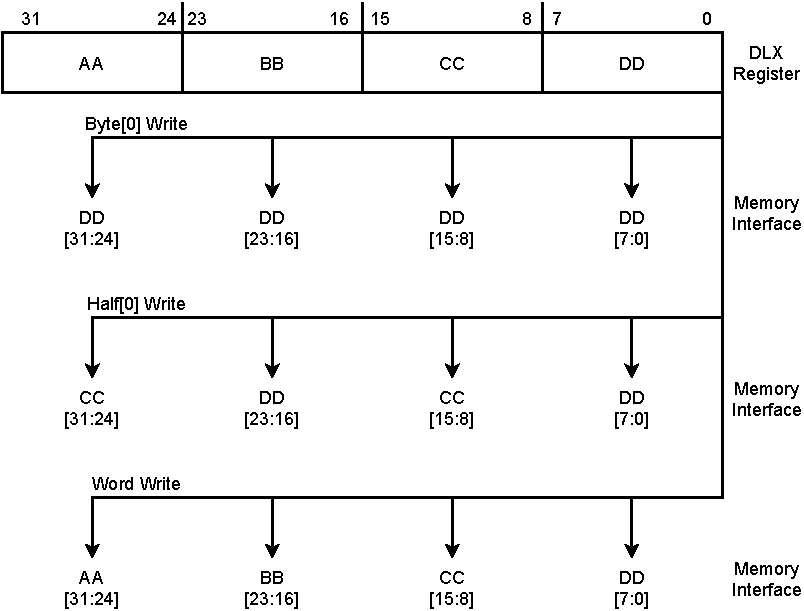
\includegraphics[width=.57\textwidth]{chapters/2_dlx/images/DLX-MemoryWordReplication.pdf}
    \caption{Data Write Replication}
    \label{figure:dlx:memory_replication}
\end{figure} 

\newpage
\section{Instruction Set}
\label{section:inst_set}

The Instruction Set supported by the DLX is made of different instructions, in particular regarding Integer operations. Instructions are on 32 bit and are grouped in 3 different types:\\

\begin{figure}[ht]
    \begin{center}
        \begin{bytefield}[endianness=big,bitwidth=0.03\linewidth]{32}
            \bitheader{0, 10, 11, 15, 16, 20, 21, 25, 26, 31} \\
            \bitbox{6}{OP CODE} & \bitbox{5}{REG SRC1} & \bitbox{5}{REG SRC2} &  \bitbox{5}{REG DEST} & \bitbox{11}{FUNC CODE} \\
        \end{bytefield}
    \end{center}
    \caption{R-Type}
    \label{fig:rtype}
\end{figure}

\begin{figure}[ht]
    \begin{center}
        \begin{bytefield}[endianness=big,bitwidth=0.03\linewidth]{32}
            \bitheader{0, 15, 16, 20, 21, 25, 26, 31} \\
            \bitbox{6}{OP CODE} & \bitbox{5}{REG SRC} & \bitbox{5}{REG DEST} &  \bitbox{16}{IMMEDIATE} \\
        \end{bytefield}
    \end{center}
    \caption{I-Type}
    \label{fig:itype}
\end{figure}

\begin{figure}[ht]
    \begin{center}
        \begin{bytefield}[endianness=big,bitwidth=0.03\linewidth]{32}
            \bitheader{0, 25, 26, 31} \\
            \bitbox{6}{OP CODE} & \bitbox{26}{IMMEDIATE} \\
        \end{bytefield}
    \end{center}
    \caption{J-Type}
    \label{fig:jtype}
\end{figure}

In particular, all of them have in common the \emph{OP CODE} field, used to identify the instruction.

\subsection{R-Type Instructions}

R-Type Instructions are called in this way because they operates only between registers. They all have in common the \emph{OP CODE} equal to \texttt{0b00000} and each instruction is differentiated from another one thanks to the \emph{FUNC CODE} field, as shown in Table \ref{table:r_type} and Table \ref{table:r_type_test}.

\begin{table}[H]
\begin{tabularx}{\textwidth}{|l|c|l|l|X|}
    \hline
    MNEMONIC & FUNC CODE & EXAMPLE & OPERATION & DESCRIPTION \\ 
    \hline
    SLL & \texttt{0x04} & \texttt{SLL R3, R2, R1} & $R3 \leftarrow R2 \ll R1$ & Logical shift left\\ 
    \hline
    SRL & \texttt{0x06} & \texttt{SRL R3, R2, R1} & $R3 \leftarrow R2 \gg R1$ & Logical shift right\\ 
    \hline
    SRA & \texttt{0x07} & \texttt{SRA R3, R2, R1} & $R3 \leftarrow R2 \gg R1$ & Arithmetic shift right\\ 
    \hline
    ROR & \texttt{0x08} & \texttt{ROR R3, R2, R1} & $R3 \leftarrow R2 \circlearrowright R1$ & Right rotation\\ 
    \hline
    ROL & \texttt{0x09} & \texttt{ROL R3, R2, R1} & $R3 \leftarrow R2 \circlearrowleft R1$ & Left rotation\\ 
    \hline
    MUL & \texttt{0x0E} & \texttt{MUL R3, R2, R1} & $R3 \leftarrow R2 * R1$ & Integer multiplication\\ 
    \hline
    ADD & \texttt{0x20} & \texttt{ADD R3, R2, R1} & $R3 \leftarrow R2 + R1$ & Integer Add\\ 
    \hline
    ADDU & \texttt{0x21} & \texttt{ADDU R3, R2, R1} & $R3 \leftarrow R2 + R1$ & Integer Add\\ 
    \hline
    SUB & \texttt{0x22} & \texttt{SUB R3, R2, R1} & $R3 \leftarrow R2 - R1$ & Integer subtraction\\ 
    \hline
    SUBU & \texttt{0x23} & \texttt{SUBU R3, R2, R1} & $R3 \leftarrow R2 - R1$ & Integer subtraction\\ 
    \hline
    AND & \texttt{0x24} & \texttt{AND R3, R2, R1} & $R3 \leftarrow R2 \texttt{\&} R1$ & Bitwise AND\\ 
    \hline
    OR & \texttt{0x25} & \texttt{OR R3, R2, R1} & $R3 \leftarrow R2 \mid R1$ & Bitwise OR\\ 
    \hline
    XOR & \texttt{0x26} & \texttt{XOR R3, R2, R1} & $R3 \leftarrow R2 \oplus R1$ & Bitwise XOR\\ 
    \hline
\end{tabularx}
\caption{R-TYPE Instructions: logical and arithmetic}
\label{table:r_type}
\end{table}

\begin{table}[H]
\begin{tabularx}{\textwidth}{|l|c|l|l|X|}
    \hline
    MNEMONIC & FUNC CODE & EXAMPLE & OPERATION & DESCRIPTION \\ 
    \hline
    SEQ & \texttt{0x28} & \texttt{SEQ R3, R2, R1} & $R3 \leftarrow R2 == R1$ & 1 if R2 equal R1\\ 
    \hline
    SNE & \texttt{0x29} & \texttt{SNE R3, R2, R1} & $R3 \leftarrow R2 != R1$ & 1 if R2 not equal R1\\ 
    \hline
    SLT & \texttt{0x30} & \texttt{SLT R3, R2, R1} & $R3 \leftarrow R2 < R1$ & 1 if R2 less R1\\ 
    \hline
    SGT & \texttt{0x31} & \texttt{SGT R3, R2, R1} & $R3 \leftarrow R2 > R1$ & 1 if R2 great R1\\ 
    \hline
    SLE & \texttt{0x32} & \texttt{SLE R3, R2, R1} & $R3 \leftarrow R2 \leq R1$ & 1 if R2 less or equal R1\\ 
    \hline
    SGE & \texttt{0x33} & \texttt{SGE R3, R2, R1} & $R3 \leftarrow R2 \geq R1$ & 1 if R2 great or equal R1\\ 
    \hline
    SLTU & \texttt{0x3A} & \texttt{SLTU R3, R2, R1} & $R3 \leftarrow R2 < R1$ & 1 if R2 unsigned less R1\\ 
    \hline
    SGTU & \texttt{0x3B} & \texttt{SGTU R3, R2, R1} & $R3 \leftarrow R2 > R1$ & 1 if R2 uns great R1\\ 
    \hline
    SLEU & \texttt{0x3C} & \texttt{SLEU R3, R2, R1} & $R3 \leftarrow R2 \leq R1$ & 1 if R2 uns less/eq R1\\ 
    \hline
    SGEU & \texttt{0x3D} & \texttt{SGEU R3, R2, R1} & $R3 \leftarrow R2 \geq R1$ & 1 if R2 uns great/eq R1\\ 
    \hline
\end{tabularx}
\caption{R-TYPE Instructions: test instructions}
\label{table:r_type_test}
\end{table}

\subsection{Pseudo R-Type Instructions}

Here we find R-Type like operations: they work only with registers but have their OPCODE.

\begin{table}[H]
\begin{tabularx}{\textwidth}{|l|c|l|l|X|}
    \hline
    MNEMONIC & OP CODE & EXAMPLE & OPERATION & DESCRIPTION \\ 
    \hline
    JR & \texttt{0x12} & \texttt{JR R1} & $PC \leftarrow PC + R1$ & PC += R31\\ 
    \hline
    JALR & \texttt{0x13} & \texttt{JALR R1} & $R31 \leftarrow PC $ & R31 = actual PC\\ 
    & & & $PC \leftarrow PC + R1$ & PC += R1\\ 
    \hline
    RET & \texttt{0x1F} & \texttt{RET} & $PC \leftarrow R31$ & PC = R31\\ 
    & & & & Context Switch begins\\ 
    \hline
    NOP & \texttt{0x15} & \texttt{NOP} & & Does exactly nothing\\ 
    \hline
    TICKTMR & \texttt{0x34} & \texttt{TICKTMR R16} &  $R16 \leftarrow TICK TIMER $ & Get Tick Timer value\\ 
    \hline
\end{tabularx}
\caption{Pseudo R-TYPE Instructions: branch, jump and mix}
\label{table:r_type_jump}
\end{table}

\subsection{J-Type Instructions}

J-Type Instructions are groups of instructions made for code jump. Thanks to the structure of these instructions, long jumps can be executed (i.e. the relative address can be very big).

\begin{table}[H]
\begin{tabularx}{\textwidth}{|l|c|l|l|X|}
    \hline
    MNEMONIC & OP CODE & EXAMPLE & OPERATION & DESCRIPTION \\ 
    \hline
    J & \texttt{0x02} & \texttt{J LABEL} & $PC \leftarrow PC + LABEL$ & PC += rel label\\ 
    \hline
    JAL & \texttt{0x03} & \texttt{JAL LABEL} & $R31 \leftarrow PC $ & R31 = actual PC\\ 
    & & & $PC \leftarrow PC + LABEL$ & PC += rel label\\ 
    \hline
    CALL & \texttt{0x1E} & \texttt{CALL LABEL} & $R31 \leftarrow PC $ & R31 = actual PC\\ 
    & & & $PC \leftarrow PC + LABEL$ & PC += rel label\\ 
    & & & & Context Switch begins\\ 
    \hline
\end{tabularx}
\caption{J-TYPE Instructions}
\label{table:j_type}
\end{table}

\newpage
\subsection{I-Type Instructions}

I-Type instructions support immediate operands, as shown in Table \ref{table:i_type_airth_logic}. 

\begin{table}[H]
\begin{tabularx}{\textwidth}{|l|c|l|l|X|}
    \hline
    MNEMONIC & OP CODE & EXAMPLE & OPERATION & DESCRIPTION \\ 
    \hline
    ADDI & \texttt{0x08} & \texttt{ADDI R3, R0, \#2} & $R3 \leftarrow R0 + 2$ & Integer Add\\ 
    \hline
    ADDUI & \texttt{0x09} & \texttt{ADDUI R3, R2, \#2} & $R3 \leftarrow R2 + 2$ & Integer Add\\ 
    \hline
    SUBI & \texttt{0x0A} & \texttt{SUBI R3, R2, R1} & $R3 \leftarrow R2 - R1$ & Integer subtraction\\ 
    \hline
    SUBUI & \texttt{0x0B} & \texttt{SUBUI R3, R2, R1} & $R3 \leftarrow R2 - R1$ & Integer subtraction\\ 
    \hline
    ANDI & \texttt{0x0C} & \texttt{ANDI R3, R2, R1} & $R3 \leftarrow R2 \texttt{\&} R1$ & Bitwise AND\\ 
    \hline
    ORI & \texttt{0x0D} & \texttt{ORI R3, R2, R1} & $R3 \leftarrow R2 \mid R1$ & Bitwise OR\\ 
    \hline
    XORI & \texttt{0x0E} & \texttt{XORI R3, R2, R1} & $R3 \leftarrow R2 \oplus R1$ & Bitwise XOR\\ 
    \hline
    LHI & \texttt{0x0F} & \texttt{LHI R3, \#0xABCD} & $R3 \leftarrow \texttt{0xABCD0000}$ & Load Upper Half\\ 
    \hline
    SLLI & \texttt{0x14} & \texttt{SLLI R3, R2, \#1} & $R3 \leftarrow R2 \ll 1$ & Logical shift left\\ 
    \hline
    SRLI & \texttt{0x16} & \texttt{SRLI R3, R2, \#1} & $R3 \leftarrow R2 \gg 1$ & Logical shift right\\ 
    \hline
    SRAI & \texttt{0x17} & \texttt{SRAI R3, R2, \#1} & $R3 \leftarrow R2 \gg 1$ & Arithmetic shift right\\ 
    \hline
\end{tabularx}
\caption{I-TYPE Instructions: logical and arithmetic}
\label{table:i_type_airth_logic}
\end{table}


\begin{table}[H]
\begin{tabularx}{\textwidth}{|l|c|l|l|X|}
    \hline
    MNEMONIC & OP CODE & EXAMPLE & OPERATION & DESCRIPTION \\ 
    \hline
    SEQI & \texttt{0x18} & \texttt{SEQI R3, R2, \#1} & $R3 \leftarrow R2 == 1$ & 1 if R2 equal 1\\ 
    \hline
    SNEI & \texttt{0x19} & \texttt{SNEI R3, R2, \#1} & $R3 \leftarrow R2 != 1$ & 1 if R2 not equal 1\\ 
    \hline
    SLTI & \texttt{0x1A} & \texttt{SLTI R3, R2, \#1} & $R3 \leftarrow R2 < 1$ & 1 if R2 less 1\\ 
    \hline
    SGTI & \texttt{0x1B} & \texttt{SGTI R3, R2, \#1} & $R3 \leftarrow R2 > 1$ & 1 if R2 great 1\\ 
    \hline
    SLEI & \texttt{0x1C} & \texttt{SLEI R3, R2, \#1} & $R3 \leftarrow R2 \leq 1$ & 1 if R2 less or equal 1\\ 
    \hline
    SGEI & \texttt{0x1D} & \texttt{SGEI R3, R2, \#1} & $R3 \leftarrow R2 \geq 1$ & 1 if R2 great or equal 1\\ 
    \hline
    SLTUI & \texttt{0x3A} & \texttt{SLTUI R3, R2, \#1} & $R3 \leftarrow R2 < 1$ & 1 if R2 unsigned less 1\\ 
    \hline
    SGTUI & \texttt{0x3B} & \texttt{SGTUI R3, R2, \#1} & $R3 \leftarrow R2 > 1$ & 1 if R2 uns great 1\\ 
    \hline
    SLEUI & \texttt{0x3C} & \texttt{SLEUI R3, R2, \#1} & $R3 \leftarrow R2 \leq 1$ & 1 if R2 uns less/eq 1\\ 
    \hline
    SGEUI & \texttt{0x3D} & \texttt{SGEUI R3, R2, \#1} & $R3 \leftarrow R2 \geq 1$ & 1 if R2 uns great/eq 1\\ 
    \hline
\end{tabularx}
\caption{I-TYPE Instructions: test instructions}
\label{table:i_type_test}
\end{table}


\begin{table}[H]
\begin{tabularx}{\textwidth}{|l|c|l|l|X|}
    \hline
    MNEMONIC & OP CODE & EXAMPLE & OPERATION & DESCRIPTION \\ 
    \hline
    LB & \texttt{0x20} & \texttt{LB R1, 40(R2)} & $R1 \leftarrow MEM[ R2 + 40 ] $ & Load Byte / Sign Ext\\ 
    \hline
    LH & \texttt{0x21} & \texttt{LH R1, 40(R2)} & $R1 \leftarrow MEM[ R2 + 40 ] $ & Load Half / Sign Ext\\ 
    \hline
    LW & \texttt{0x23} & \texttt{LW R1, 40(R2)} & $R1 \leftarrow MEM[ R2 + 40 ] $ & Load Word / Sign Ext\\ 
    \hline
    LBU & \texttt{0x24} & \texttt{LBU R1, 40(R2)} & $R1 \leftarrow MEM[ R2 + 40 ] $ & Load Byte\\ 
    \hline
    LHU & \texttt{0x25} & \texttt{LHU R1, 40(R2)} & $R1 \leftarrow MEM[ R2 + 40 ] $ & Load Half\\ 
    \hline
    SB & \texttt{0x28} & \texttt{SB 40(R2), R1} & $MEM[ R2 + 40 ] \leftarrow R1 $ & Store Byte \\ 
    \hline
    SH & \texttt{0x29} & \texttt{SH 40(R2), R1} & $MEM[ R2 + 40 ] \leftarrow R1 $ & Store Half \\ 
    \hline
    SW & \texttt{0x2B} & \texttt{SW 40(R2), R1} & $MEM[ R2 + 40 ] \leftarrow R1 $ & Store Word \\ 
    \hline
\end{tabularx}
\caption{I-TYPE Instructions: Load \& Store}
\label{table:i_type_loadstore}
\end{table}

\begin{table}[H]
\begin{tabularx}{\textwidth}{|l|c|l|l|X|}
    \hline
    MNEMONIC & OP CODE & EXAMPLE & OPERATION & DESCRIPTION \\ 
    \hline
    BEQZ & \texttt{0x04} & \texttt{BEQZ R1, LABEL} & $PC \leftarrow PC + LABEL$ & $R1 = 0$ ?\\ 
    & & & & PC += label\\
    \hline
    BNEZ & \texttt{0x05} & \texttt{BNEZ R1, LABEL} & $PC \leftarrow PC + LABEL$ & $R1 \neq 0$ ?\\ 
    & & & & PC += label\\
    \hline
    BGT & \texttt{0x30} & \texttt{BGT R1, R2, LABEL} & $PC \leftarrow PC + LABEL$ & $R1 > R2$ ?\\ 
    & & & & PC += label\\
    \hline
    BGE & \texttt{0x31} & \texttt{BGE R1, R2, LABEL} & $PC \leftarrow PC + LABEL$ & $R1 \ge R2$ ?\\ 
    & & & & PC += label\\
    \hline
    BLT & \texttt{0x32} & \texttt{BLT R1, R2, LABEL} & $PC \leftarrow PC + LABEL$ & $R1 < R2$ ?\\ 
    & & & & PC += label\\
    \hline
    BLE & \texttt{0x33} & \texttt{BLE R1, R2, LABEL} & $PC \leftarrow PC + LABEL$ & $R1 \le R2$ ?\\ 
    & & & & PC += label\\
    \hline
\end{tabularx}
\caption{I-TYPE Instructions: Conditional Branch Instructions}
\label{table:i_type_branch}
\end{table}
\chapter{Fetch Stage}
The first stage of the DLX pipeline is the Fetch Stage, which has been included directly inside the \texttt{DLX}. It is used to manage the current Program Counter \texttt{PC} and send it out to the memory to fetch the instruction from it and save the instruction into the Instruction Register \texttt{IR}. At each clock cycle, the new \texttt{PC} is computed by summing 4, since the instructions are on 32 bits and the memory is organized in words of 1 byte. This can be summarized in the following way:
\begin{align*}
    IR &\leftarrow MEM[PC]\\
    NPC &\leftarrow PC + 4
\end{align*}
As will be explained in the Jump and Branch Management section (refer to \ref{sec:jmp_branch}), to manage jumps and conditional branches, some additional hardware is necessary in order to compute the new address.

\section{Instruction Register}
The Instruction Register (\texttt{IR}) is, in this case, a 32 bits register that is used to store the instruction (that is in fact on 32 bits) that comes from the Instruction RAM.

During the normal operation, this register is updated with the new instruction coming from the IRAM, but this is not always true. We have two cases in which the register is not updated:
\begin{enumerate}
    \item When \texttt{i\_IR\_LATCH\_EN} is at 0, in fact, this signal is used to avoid updating the value inside the \texttt{IR}. During the instruction execution, it could be that the DRAM is not ready, a signal \texttt{i\_DRAM\_NOTREADY} is checked inside the Control Unit and in case of `1' the \texttt{i\_IR\_LATCH\_EN} is put at 0. In this way, everything is stalled so the CW in the pipeline and the Instruction Register will remain the same until the DRAM will become ready again. 
    \item When the reset signal is asserted or when the \texttt{i\_IR\_STALL} is at one (this signal is at one when the pipeline must continue its execution but a NOP is executed for resolving a hazard), a ``bubble" is added to the pipeline. So, the Instruction Register will contain the \texttt{x"54000000"} value. This is used in order to manage the jump and branch instructions. A more detailed description is available at section \ref{sec:jmp_branch}.
\end{enumerate}

\section{Program Counter}
As anticipated before, the Program Counter (\texttt{PC}) is the address used to fetch the instruction from the IRAM and it is on 32 bits. Thus it can address up to 4GB.

At each clock cycle, the current Program Counter is updated with the \texttt{NPC} computed in the Decode stage in order to point to the next instruction. This allows managing both the standard execution, by adding 4 to the current \texttt{PC}, subtracting/adding an offset, or set it to an immediate. Only in case of reset, it is set to 0 otherwise, it will be set to the value of the new Program Counter, computed in the Decode stage. In a specular way, from what is done for the Instruction Register, the \texttt{PC} is updated only when the \texttt{i\_PC\_LATCH\_EN} is `1'.

\section{Jump and Branch Management}
\label{sec:jmp_branch}
Jumps and branches are crucial instructions to build a program, but their management from the point of view of the pipeline is not straightforward. Therefore, the Fetch Stage must be able to manage three additional signals:
\begin{enumerate}
    \item \texttt{i\_PC\_LATCH\_EN}: this signal is used to avoid updating the PC with the new one coming from the Decode Stage. The update is inhibited when the instruction is a jump or when \texttt{i\_IR\_LATCH\_EN} is `0'. 
    \item \texttt{i\_IR\_LATCH\_EN}: it is used to avoid updating the Instruction Register. This happens when:
    \begin{itemize}
        \item A Data Hazard occurs
        \item A \texttt{CAL} instruction is executed and we have to wait for a spill operation to be completed
        \item A \texttt{RET} instruction is executed and we have to wait for a fill operation to be completed
    \end{itemize}
    It's important to say that, when the \texttt{IR} is not updated, the \texttt{PC} is not updated too.
    \item \texttt{i\_IR\_STALL}: a NOP is inserted in the pipeline in order to manage the jump and the branch instructions. This is due to the control hazards; when a branch is executed, it may or may not change the PC to something other than its current value plus 4. As it will be described more precisely in the Decode Stage section, the computation of the new PC, both for branch and jump, is done there. For this reason, it is updated only at the end of the Decode Stage, and, if not blocked, a wrong instruction is fetched.
    
    The solution this DLX implements is to add a NOP not to execute a wrong instruction.
\end{enumerate}
\chapter{Decode Stage}

\section{Instruction Decode}
\section{Register File and Windowing}
The general structure of a register file is based on a decoder that takes the selection input (so the address of the desired register) and enables it (using also the enable signal). At this point, an input signal will contain the value to be written. On the other hand, a read signal is used to select among all the registers.\newline\newline
The DLX presented in this document has been enhanced in order to be able to manage subroutine in a transparent manner from the point of view of the user. For this reason, the DLX must be able to handle subroutines, and so the context switching, that consists in saving the
registers content in order to be restored once the procedure has been completed. The straightforward solution is to save into the memory all registers but this is not feasible in terms of delay, since for 32 registers we will need 32 clock cycles; if you image this in a pipeline, this corresponds to a long stall each time a procedure is called.

A windowed register allows to reduce the overhead due to the context switch; the basic idea
is to split the available registers in the physical register file into blocks, called \textit{windows}. We have limited amount of physical registers in the register file, for this reason a finite number of windows are defined. Each window is assigned to a subroutine, so that the procedure can write only on those register. This is transparent from the point of view of the CPU, that sees all registers available. Thus, the physical register file has a wrapper around it with a logic and a Register Management Logic (MML) that allows to perform the translation between the CPU requests to corresponding window for the running procedure.\newline\newline
What if the number of called procedure is larger than the number of available windows? The main
memory is involved only when there are no free windows in the register file. In this case, the oldest allocated window is swapped into the main memory, so that the new one can be allocated. Obviously, once all the recursion chain has been unrolled, the swapped window in the memory must be restored into the register file.
All windows, so each procedure, has 4 blocks of 8 registers each one:
\begin{enumerate}
	\itemsep0sp
	\item \textbf{IN}: the first block is dedicated to the data inherited from the parent routine (OUT);
	\item \textbf{LOCALS}: contains the registers that are dedicated to the procedure;
	\item \textbf{OUT}: is dedicated to the variables to be passed to the child routine, that is the IN of the next sub-procedure
	\item \textbf{GLOBAL}: the last block is common to every windows.
\end{enumerate}
When a procedure is called, the first LOCALS and OUT blocks are allocated from the physical file register and assigned to it (because IN is the OUT of the previous one).

By calling many nested procedures, at some point there will be no free windows; for this reason the oldest is de-allocated from the physical FR and swapped to the main memory, the operation is called \textbf{SPILL}. This it accomplished by using a support pointer, called \textbf{Saved Window Pointer SWP} that stores the point of the spilled data, exactly the end of the LOCALS block (only IN and LOCAL are spilled, the OUT block is not spilled because is the IN of the next sub-procedure). In practice it define the position of the last free cell. Notice that this operation cannot be executed in one clock cycle: each register is spilled once at a clock cycle.\newline\newline
On the other hand, when the last procedure in the chain is finished, the other are unrolled; if some of them have been spilled, a \textbf{FILL} must be executed before the actual execution. This can be achieved by, firstly decrement CWP by 16 and check if now CWP $>>$ SWP.\newline\newline
It's important to notice that the implementation of the entire register file has been implemented in Structural. Is is composed by several components:
\begin{itemize}
	\item \textbf{Decoder}: it is used to generate a single enable signal from a signal on \textbf{NBIT\_ADD} bits; in this way, a register is selected in order to perform a write. The register will check also if a write is requested;
	\item \textbf{Connection matrix}: this block allows to ``highlight" the active windows, the block IN, LOCAL and OUT will be the default destination when writing and reading;
	\item \textbf{Register file}: this block corresponds to the physical registers, composed by rows of Flip-Flops;
	\item \textbf{Select block}: this block is used for the reading, is connected to all the registers and selects, using the read address, the single register to be read;
	\item \textbf{Address generator}: this block is used only when perform a FILL or a SPILL, it generates the address for the registers to be moved from/to the memory. The memory, in this case works exactly like a stack.
\end{itemize}
Additional, but less complex components, have been used in order to manage the management of the CWP and SWP.


\subsection{Decoder}
This block receives as input the \emph{write address} on \textbf{NBIT\_ADD} bits and outputs \(\mathbf{2^{NBIT\_ADD} - 1} \) bits. It has the utility of converting the address of the register at which we need to write into its enable signal. 

The idea is that if the input is \(0b00010\) the output will be \(0b00000000000000000000000000000100\). In fact if the input is decimal 2, it means that we need to write the second register of the \emph{GLOBAL} block. In terms of enable it can be translated by having the bit with index 2 at one. In fact in the output we see that the it with index 2 has value 1, while the others are all 0. 

The output is divided (in the schematic) in order to represent the group of bits. In particular we have that: 
\begin{itemize}
    \item M - 1 DOWNTO 0: bits associated to the \emph{GLOBAL} register
    \item M + N - 1 DOWNTO M: bits associated to the \emph{IN} register
    \item M + 2N - 1 DOWNTO M + N: bits associated to the \emph{LOCAL} register
    \item M + 3N - 1 DOWNTO M + 2N: bits associated to the \emph{OUT} register
\end{itemize}

On the top of the schematic (\autoref{decoder}) we can see an AND logic port between \emph{ENABLE} and \emph{WR} signals. If both \emph{ENABLE} and \emph{WR} are 1, it means that our register need to work. In fact, the output of the dedocer is anded with 1 and so we maintain the value. Otherwise, if one signal between \emph{ENABLE} and \emph{WR} is 0, the output will be 0 and so the AND with the output of the \emph{decoder} will return all 0. 

This signal goes into the \emph{connection matrix}, which is the next block described. 

%% MAKE FONT BIGGER
\begin{figure}[ht]
    \centering
    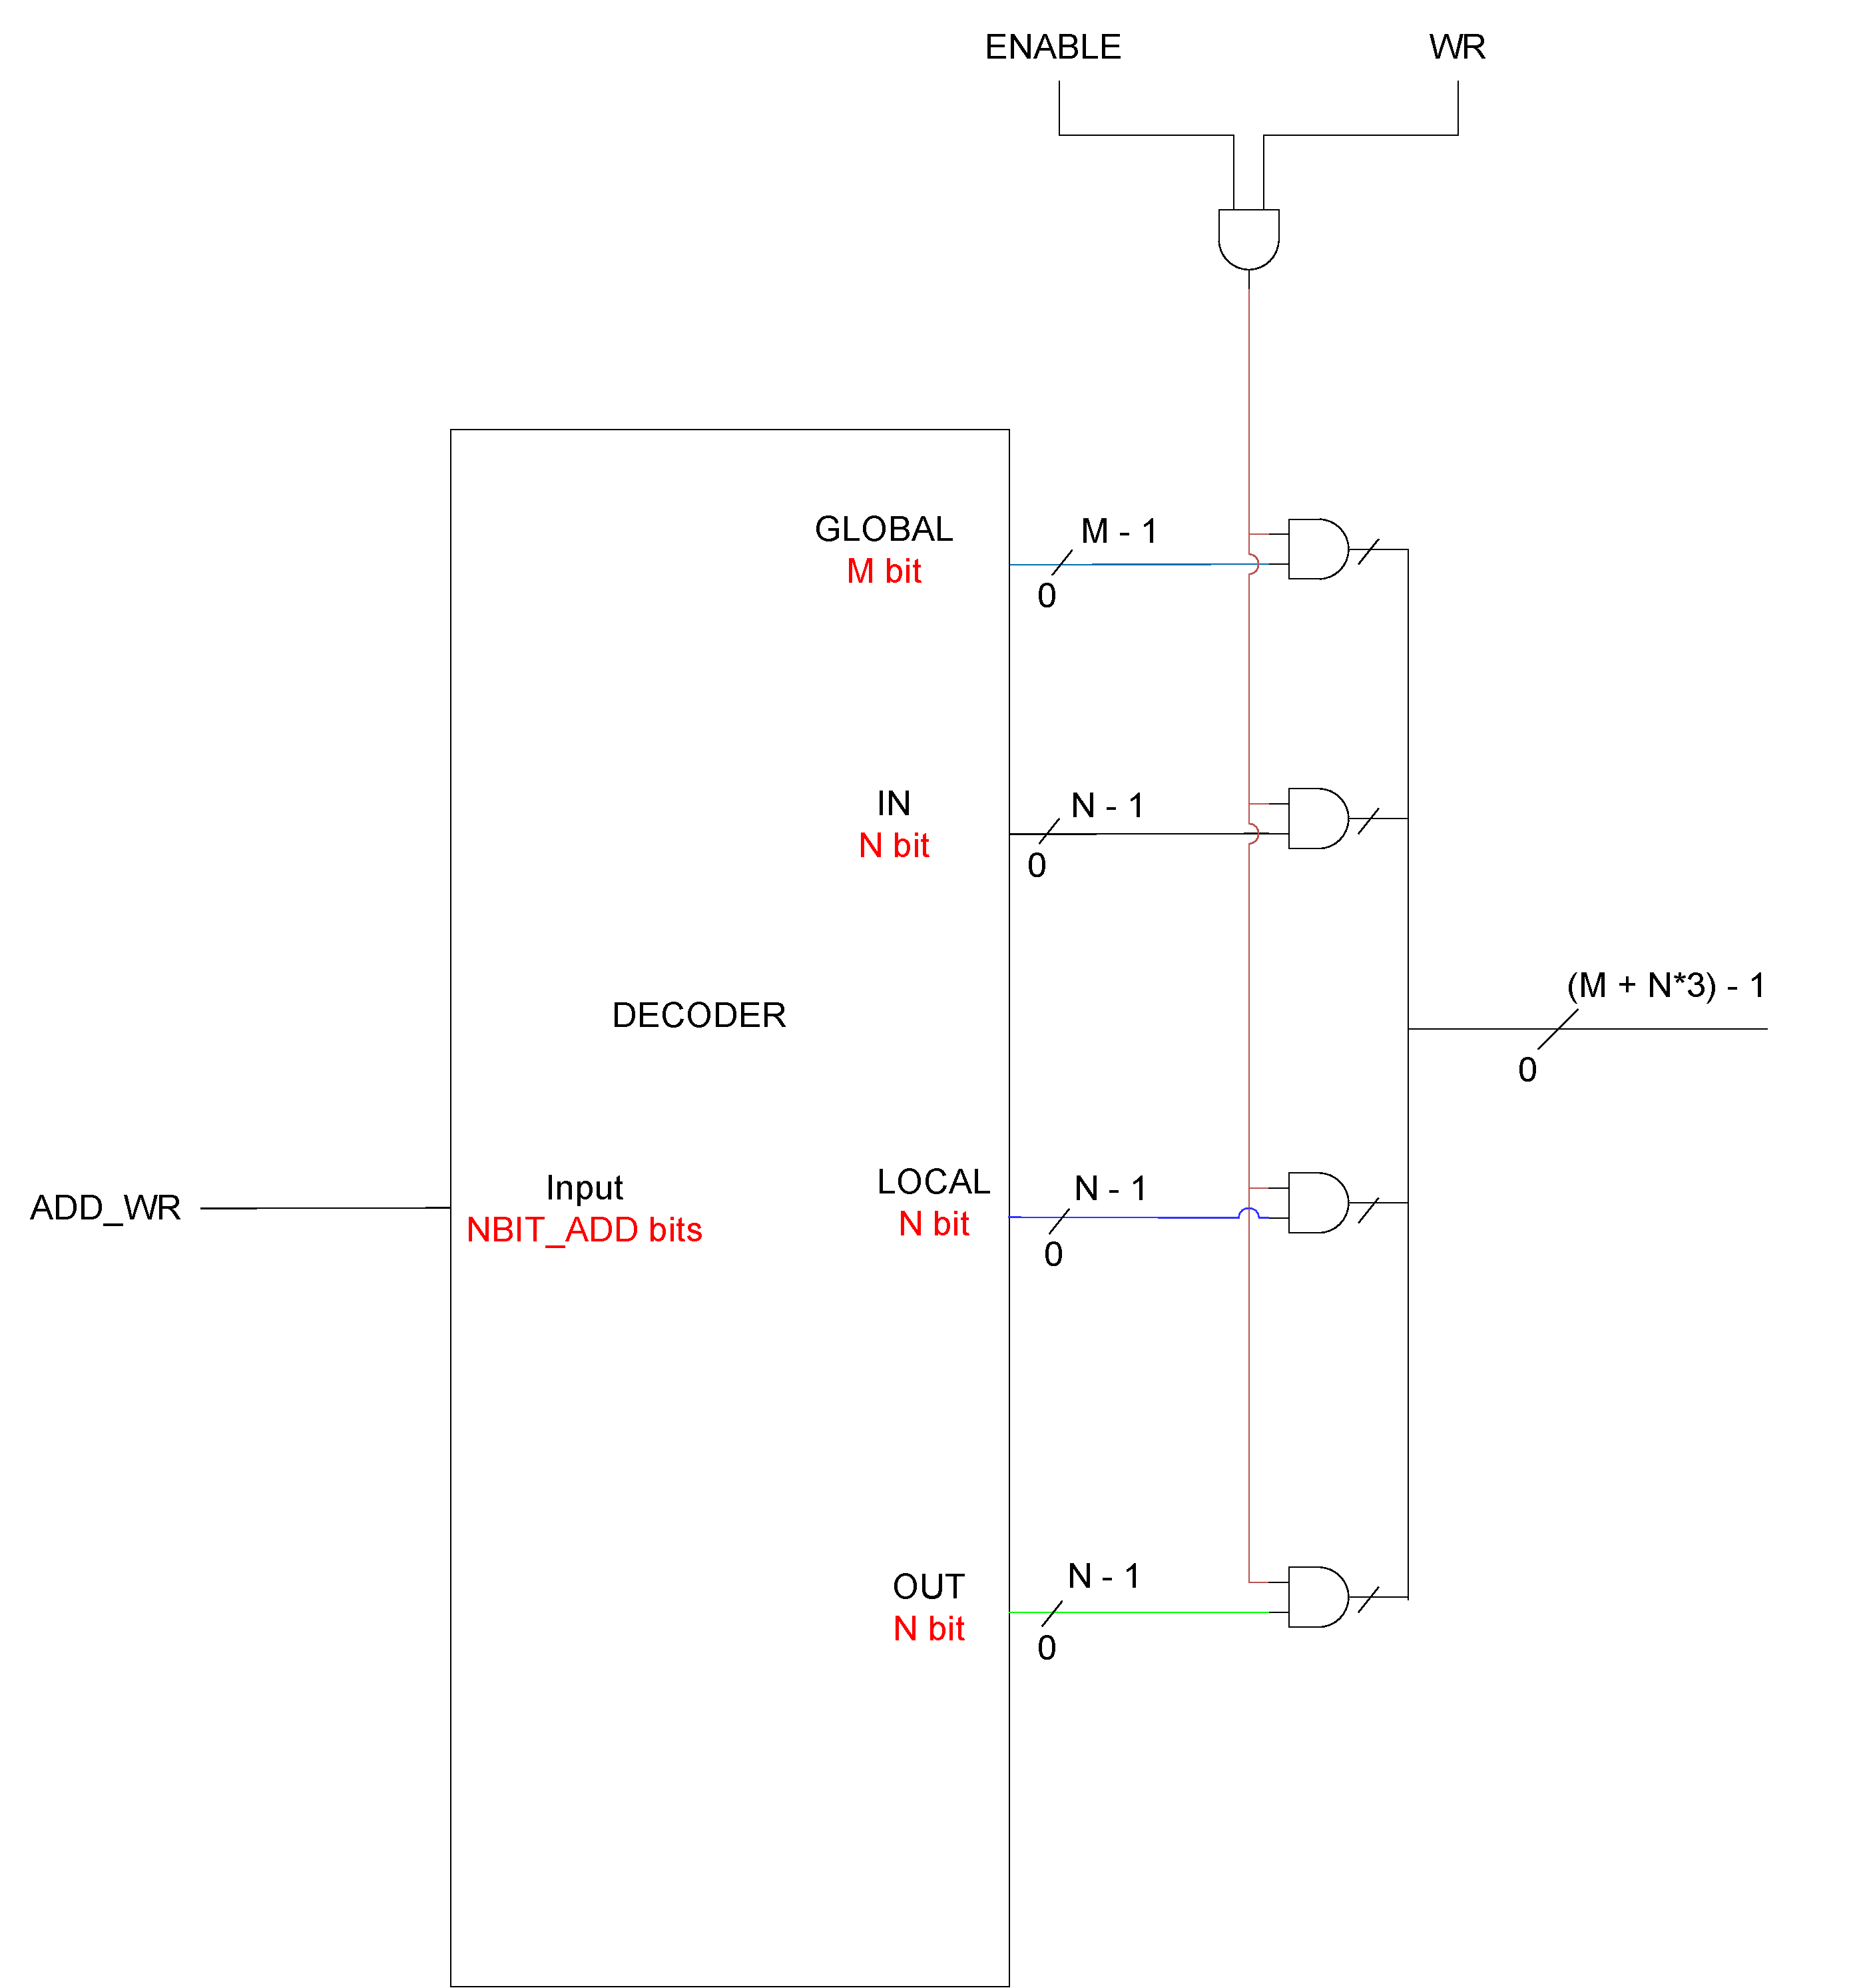
\includegraphics[width=0.7\textwidth]{chapters/4_DecodeStage/images/Decoder.pdf}
    \caption{Schematic of the Decoder}
    \label{decoder}
\end{figure}
%% MAKE FONT BIGGER

\subsection{Connection Matrix}

With the previous block, we generated all our enable signals. The problem is that we have more windows. So how do we decide which window needs to be activated? Here comes the connection matrix. This block receives as inputs the signal coming from the decoder, the current window, the saved window and the address for the pop (fill) operation. The output is a signal that contains the enable signals ready for all the registers of all windows. 

We have a specific structure for each block:
\begin{itemize}
  \item GLOBAL: the global is the simplest, because it is connected directly to the output
  \item IN: for this block we AND the IN bits coming from the decoder with the bit (that is extended) of the related window. For example if we are evaluating the IN of the first window, we will AND the IN bits with the bit 0 of the current window.
  \item OUT: for this block we AND the OUT bits coming from the decoder with the bit (that is extended) of the previous related window. For example if we are evaluating the OUT of the first window, we will AND the OUT bits with the bit 4 of the current window (supposing our window has 5 bits).
  \item LOCAL: for this block we AND the LOCAL bits coming from the decoder with the bit (that is extended) of the related window. For example if we are evaluating the LOCAL of the first window, we will AND the LOCAL bits with the bit 0 of the current window.
\end{itemize}

For the IN and OUT we then an OR between the two outputs (the logic can be seen in the schematic), while for the LOCAL we don't have anything.

In addition to that, the connection matrix also manages the saved window, used for the pop (fill) operation. First we need to invert the addr\_pop, because when we execute the pop operation, we restore data starting from the last one (we are using a STACK).
The addr\_pop\_inverted is composed like this:
\begin{itemize}
  \item 2N - 1 DOWNTO 0: we have the IN bits 
  \item N - 1 DOWNTO 0: we have the LOCAL bits
\end{itemize}

The signal is splitted into two wires and is anded with the saved related saved window pointer. 

In the end, we definitely OR the output of the previously described OR with the output of this AND. This is visible in \autoref{connection_matrix}

\begin{figure}[ht]
  \centering
  \addtolength{\leftskip}{-3cm}
  \addtolength{\rightskip}{-3cm}
  \includegraphics[width=1.4\textwidth]{chapters/4_DecodeStage/images/connection_matrix.pdf}
  \caption{Connection matrix}
  \label{connection_matrix}
\end{figure}

\newpage

\subsection{Register File}

The next block is the Register File, that is a sequence of registers. The important thing to notice in our design is how we managed the data that goes into the registers. We have two choices, data\_in and from\_mem. In order to choose we decided to use multiplexers. 
We have a multiplexer for each window. The signal used to drive the multiplexer is the saved window pointer, rotated right by 1 position and anded with the pop signal. In fact, we select from\_mem only when the pop signal is 1, otherwise we need to select data\_in. 
We use the saved window pointer shifted right by 1 because when the saved window pointer is, for example 00010 we need to restore the window 00001. 

Indeed, for dataout there are no multiplexers, because there is no choice. 

\subsection{Select Block}

This block is very simple and straightforward. It receives as input the current window, and the output of the register file (of all windows). The it selects the bit of the IN, LOCAL, OUT of the current window. The interface is shown in \autoref{select_block}.

\begin{figure}[ht]
  \centering
  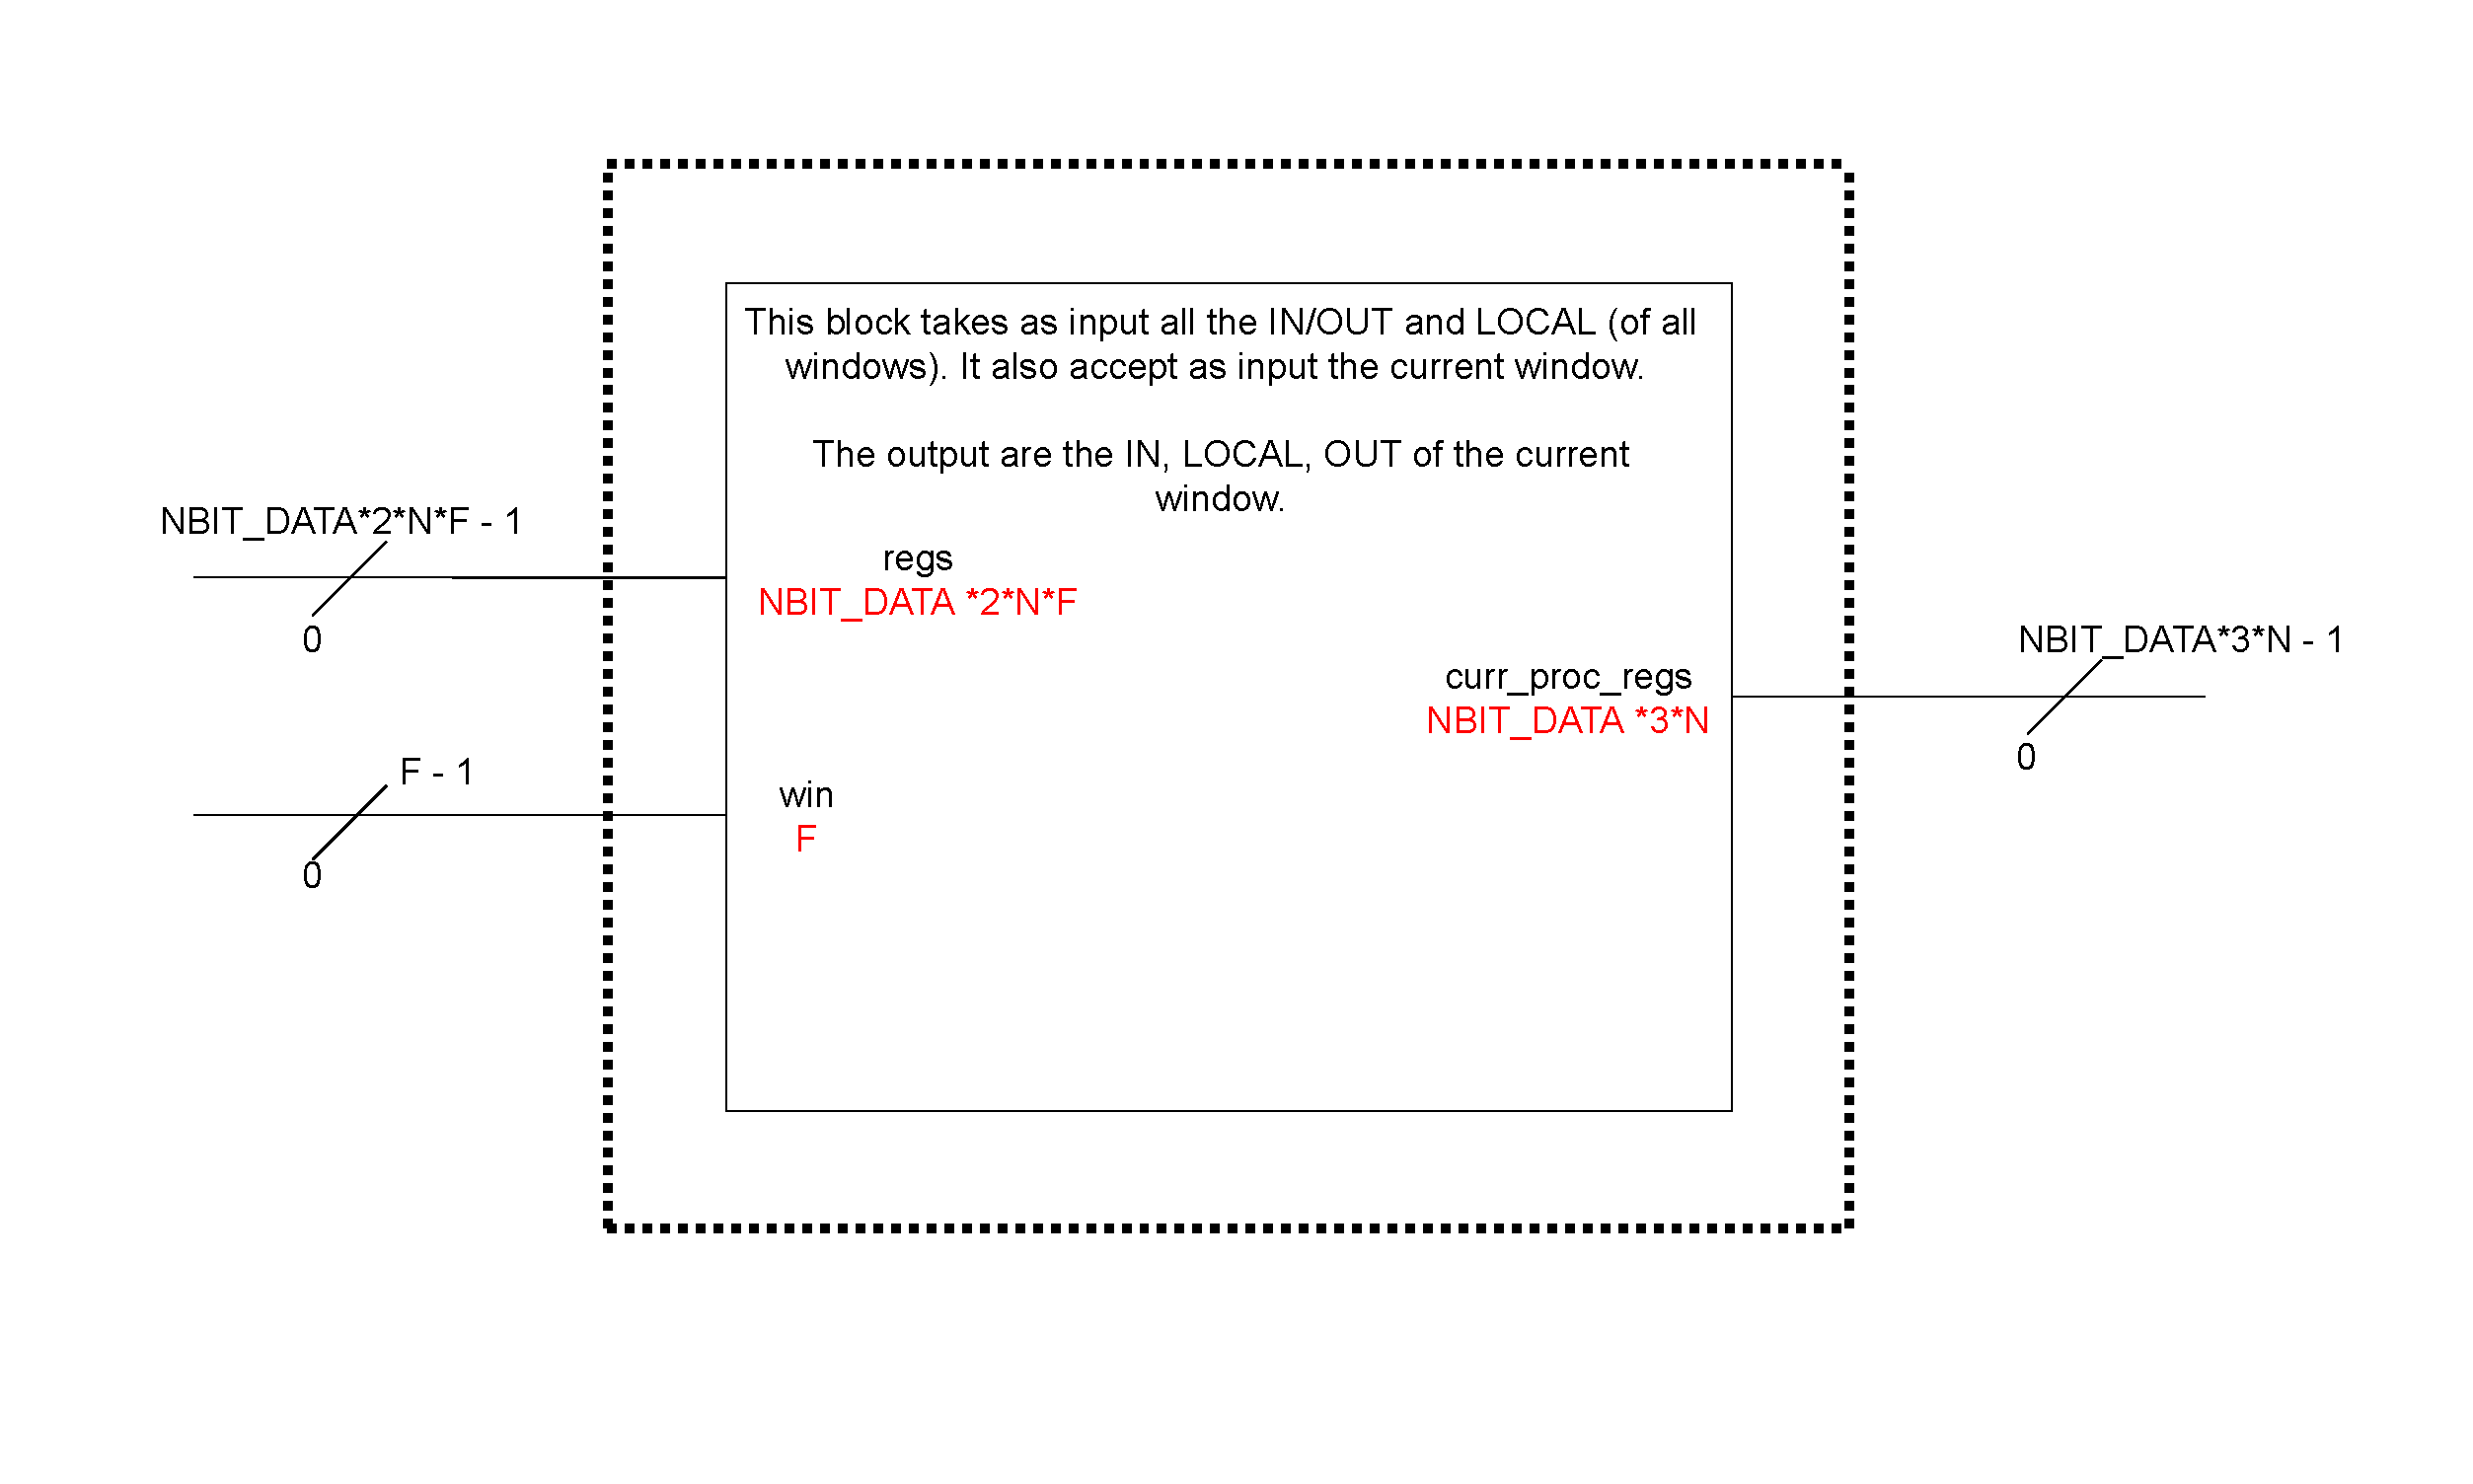
\includegraphics[width=0.65\textwidth]{chapters/4_DecodeStage/images/select_block.pdf}
  \caption{Interface of the select block}
  \label{select_block}
\end{figure}

\subsection{Output Selection}
This is the stage that decide the two output Data1\_Out and Data2\_Out. The design is shown in \autoref{output_choice}.

\begin{figure}[H]
  \centering
  \includegraphics[width=0.65\textwidth]{chapters/4_DecodeStage/images/output_choice.pdf}
  \caption{Design of the output selection}
  \label{output_choice}
\end{figure}

This stage receives the IN, LOCAL, OUT of the current window, thanks to the select block and the GLOBAL. The two addresses, ADD\_RD1 and ADD\_RD2, select the output of the multiplexer which goes into the register, used to respect the timing. The Enable of each register is the and of the ENABLE and the RD signal. The decision was made in order to stop reading when the circuit is not enabled, and so to have a granural and precise control of the circuit.

\subsection{Next Window Calculator}

This block is used to compute the next window, both for the current window and the saved window. The schematic is shown in \autoref{nwin_cal}.

\begin{figure}[H]
  \centering
  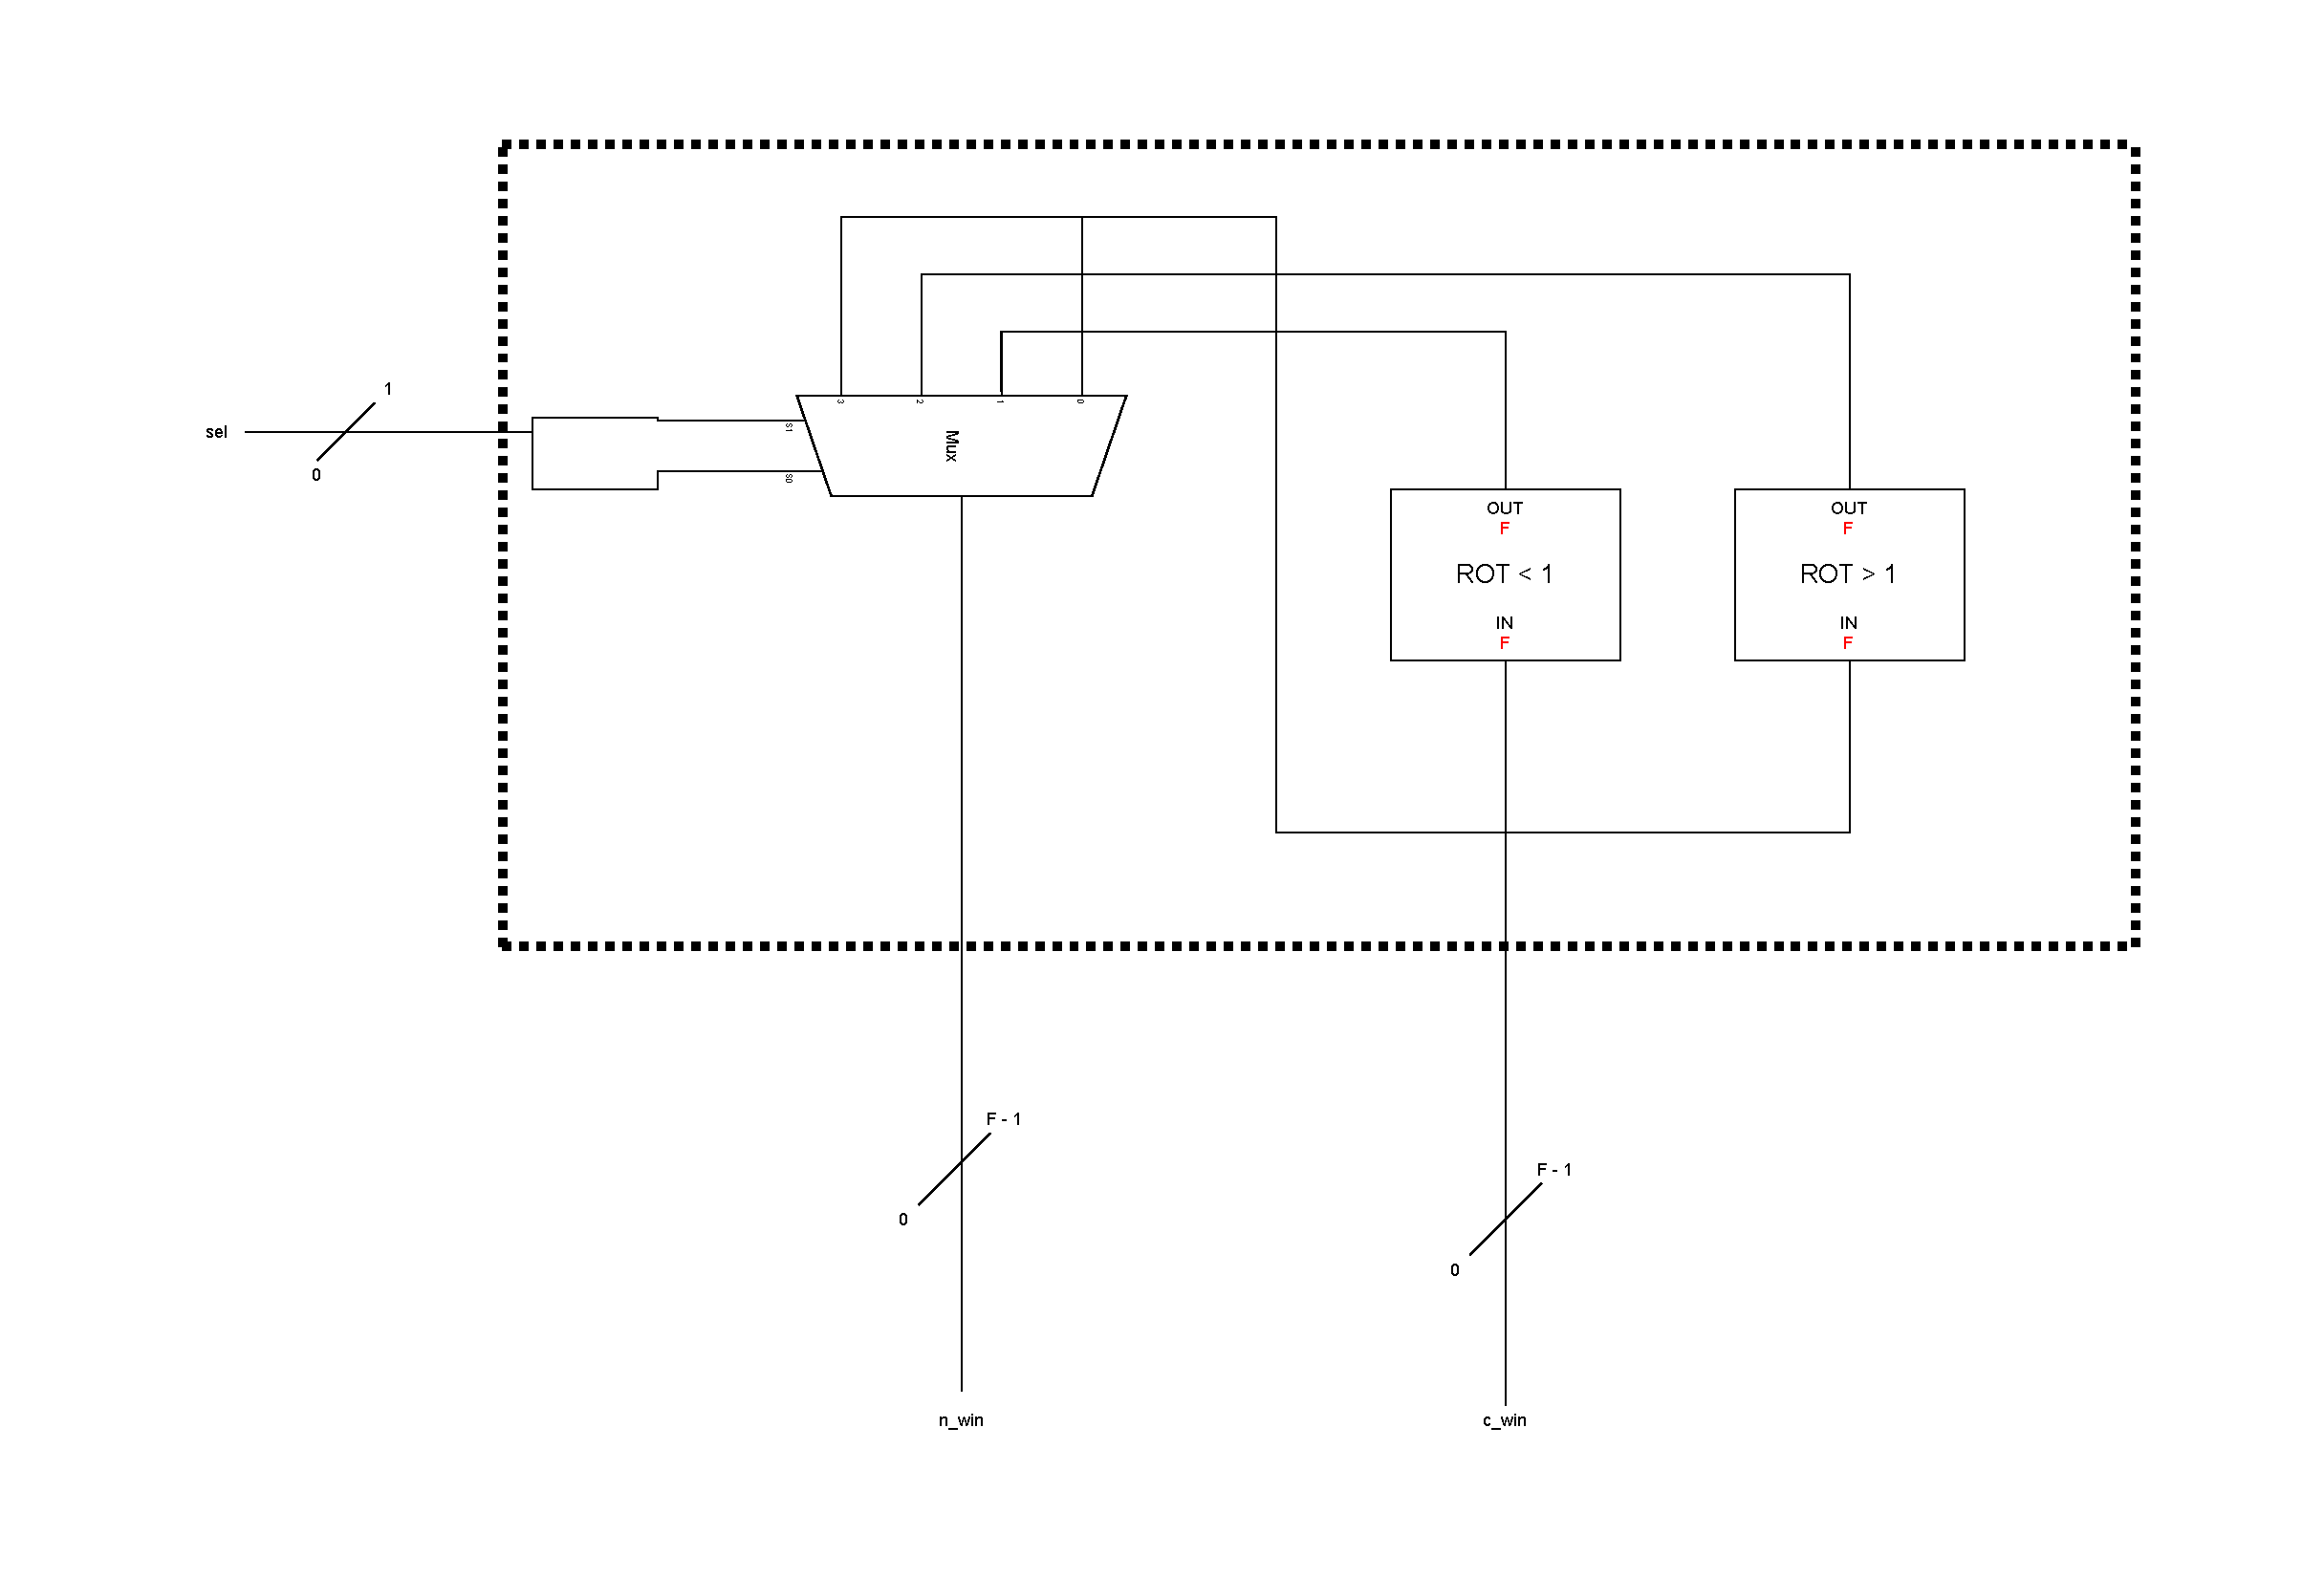
\includegraphics[width=1\textwidth]{chapters/4_DecodeStage/images/nwin_cal.pdf}
  \caption{Design of the next window calculator}
  \label{nwin_cal}
\end{figure}

Inside this block there is a logic able to rotate right or left and a multiplexer, that allows to select the correct output based on what the circuit needs. 

\section{Hazard Control}
\section{Comparator}
\label{sec:comparator}
The straightforward way to implement a comparator, allows only to check if two operands, \texttt{A} and \texttt{B}, are equals. The solution is sketched at figure \ref{fig:comparator_basic}, that is based on $N$ XNOR, where $N$ is the number of bits of the operands and an AND gate with $N$ inputs.

Even if this solution is extremely compact, it allows to perform only the equality comparison; since this DLX implementation has the ability to perform complex conditional branch instructions (refer to the Instruction section \ref{section:inst_set}) and conditional set instructions (refer to the Set-Like Operations Unit \ref{section:set_link_operations_unit}) we need a more complex solution. In fact, if we need to perform a jump only if \texttt{A} $>$ \texttt{B} (strictly greater) we need to check exactly this precise condition.

\begin{figure}[H]
	\centering
	\begin{minipage}{.5\textwidth}
		\centering
		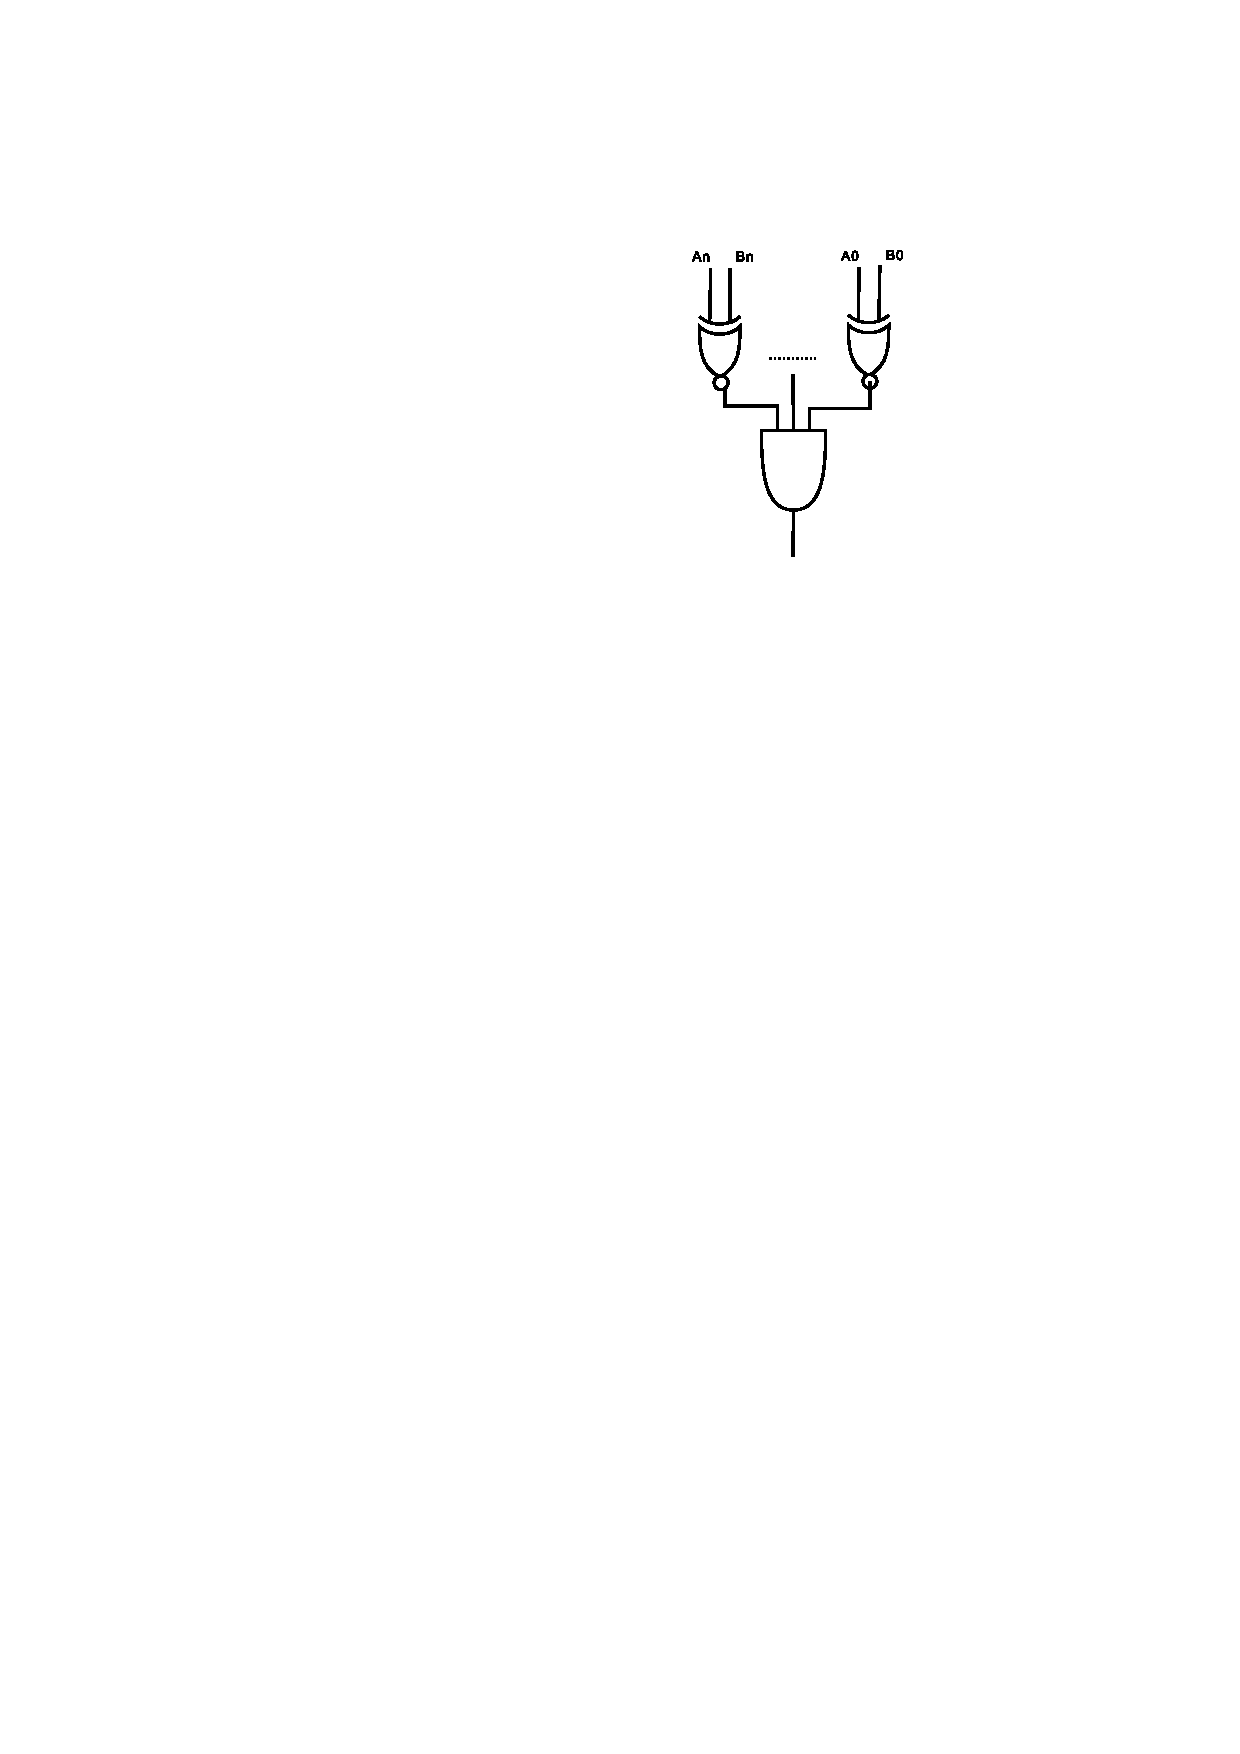
\includegraphics[width=0.55\textwidth]{chapters/4_DecodeStage/images/comparator_basic.pdf}
		\caption{Design of the basic comparator}
		\label{fig:comparator_basic}
	\end{minipage}%
	\begin{minipage}{.5\textwidth}
		\centering
		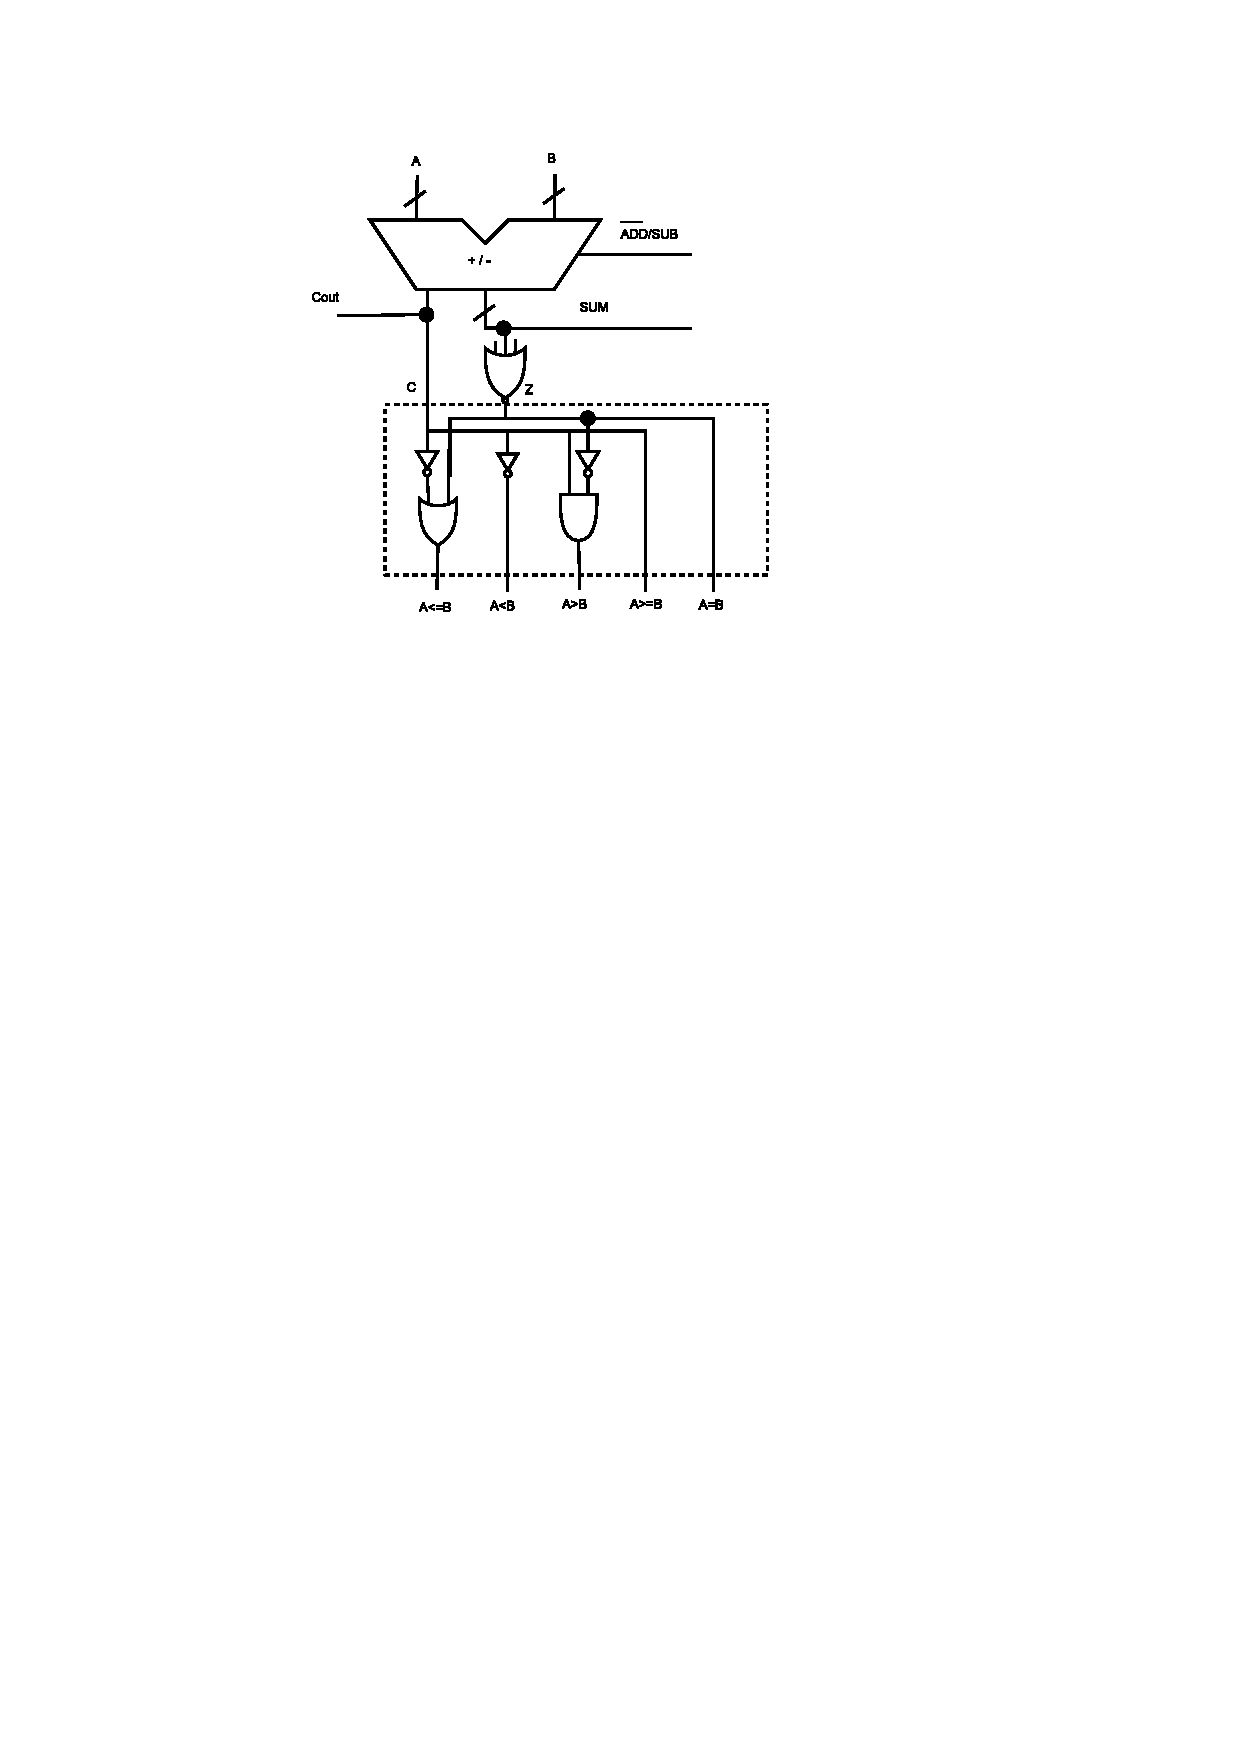
\includegraphics[width=0.7\textwidth]{chapters/4_DecodeStage/images/comparator_advanced.pdf}
		\caption{Design of the advanced comparator}
		\label{comparator_advanced}
	\end{minipage}
\end{figure}

The advance comparator exploits the comparison by performing a subtraction between \texttt{A} and \texttt{B} and then checking the result. This DLX implementation is based on a P4 adder that is able to perform subtraction and then a set of checks, the same that are in the \ref{comparator_advanced} are performed in order to generate the comparison outputs. We can perform the comparisons using this boolean equations, where $C$ is the carry-out and $Z$ is the zero check (all bits of the results are zeros):
\begin{align*}
	A > B &\rightarrow C \cdot \overline{Z}\\
	A \geq B &\rightarrow C\\
	A < B  &\rightarrow \overline{C}\\
	A \leq B &\rightarrow \overline{C} + Z\\
	A = B &\rightarrow Z\\
	A \neq B  &\rightarrow \overline{Z} 
\end{align*}

 In order to avoid to propagate six different signal, the outcomes of the comparisons are encoded into a signal \texttt{LGET} on two bits. The encoded value are the ones in the \ref{tab:lget} table.
 \begin{multicols}{2}
 	\begin{table}[H]
 		\begin{center}
 			\begin{tabular}{ c| c}
 				\texttt{LGET} & Case\\
 				\hline
 				01 & $A < B$ \\
 				00 & $A \leq B$ \\
 				11 & $A > B$ \\
 				10 & $A \geq B$
 				
 			\end{tabular}
 			\caption{LEQ encoding}
 			\label{tab:lget}
 		\end{center}
 	\end{table}
 	
 	\columnbreak
 	
 	\begin{lstlisting}[style=vhdl,caption={VHDL code for the encodig},label=lget_code]
 	LGET <= "01" when (a_l_b = '1') else
	 	"00" when (a_le_b = '1') else 
	 	"11" when (a_g_b = '1') else
	 	"10" when (a_ge_b = '1') else
	 	"00";
 	\end{lstlisting}
 \end{multicols}

The ordering of the comparison in the \texttt{when} statement is not casual nor follows the normal patterns but, the strictly lower comparison is done before the lower equals one, because, if the latter one is true it means that is also \texttt{A} lower than \texttt{B} but not vice-versa. Using this encoding, we can simply check the second bit in order to understand if \texttt{A} $\leq$ \texttt{B} or \texttt{A} $\geq$ \texttt{B}; instead, if we want to check only $<$ or $>$ comparisons we have to check also the first bit.

 

A further improvement has been done to the advanced comparator in order to manage comparison between both signed and unsigned numbers. The carry value works like this:
\begin{itemize}
  \item Carry = 1: if \(A > B\) in unsigned
  \item Carry \(=\) 0: if \(A \leq B\) in unsigned
\end{itemize}

The advanced comparator works with unsigned numbers only. So it simply needs to be adapted for cases in which signed comparison and unsigned comparison are different. They are shown in the \autoref{comparator_cases} highlighted in red. 
It is easy to notice that in the red lines A and B always have different sign. The logic must work when the UNSIG\_SIGN\_N bit is 0, that means the circuit is dealing with a signed number. In this case the carry bit must be complemented. Knowing this things, it's easy to derive the following logic:

\begin{verbatim}
  i_cout_masked <= Cout xor (not(UNSIG_SIGN_N) and (A(A'length-1) xor B(B'length-1)));
\end{verbatim}

\begin{table}[H]
  \centering
  \begin{tabular}{c|c|c|c|c}
      \textbf{A} & \textbf{B} & \textbf{Carry out} & \textbf{Signed comparison} & \textbf{Unsigned comparison} \\
      \hline
      2 & 3 & 0 & Less & Less \\
      4 & 3 & 1 & Greater & Greater \\
      3 & 3 & 1 & Equal & Equal \\
      \rowcolor{red!50}
      -3 & 3 & 1 & Less & Greater \\
      \rowcolor{red!50}
      -2 & 3 & 1 & Less & Greater \\
      \rowcolor{red!50}
      -5 & 3 & 1 & Greater & Greater \\
      \hline
      3 & 2 & 1 & Greater & Greater \\
      3 & 4 & 0 & Less & Less \\
      3 & 3 & 1 & Equal & Equal \\
      \rowcolor{red!50}
      3 & -3 & 0 & Greater & Less \\
      \rowcolor{red!50}
      3 & -2 & 0 & Greater & Less \\
      \rowcolor{red!50}
      3 & -5 & 0 & Greater & Less \\
      \hline
      \rowcolor{red!50}
      2 & -3 & 0 & Greater & Less \\
      \rowcolor{red!50}
      4 & -3 & 1 & Greater & Less \\
      \rowcolor{red!50}
      3 & -3 & 1 & Greater & Less \\
      -3 & -3 & 1 & Equal & Equal \\
      -2 & -3 & 1 & Greater & Greater \\
      -5 & -3 & 1 & Less & Less \\
      \hline
      \rowcolor{red!50}
      -3 & 2 & 1 & Less & Greater \\
      \rowcolor{red!50}
      -3 & 4 & 0 & Less & Greater \\
      \rowcolor{red!50}
      -3 & 3 & 1 & Less & Greater \\
      -3 & -3 & 0 & Equal & Equal \\
      -3 & -2 & 0 & Less & Less \\
      -3 & -5 & 0 & Greater & Greater \\
  \end{tabular}
  \caption{All cases of possible comparison}
  \label{comparator_cases}
\end{table}
So, we the final unit corresponds to the one at figure \ref{comparator_advanced} with an additional encoder before the output, that encode the six conditions into a signal on two bits. The resulting schema is the one in figure \ref{cmp_final}.

\begin{figure}[H]
	\centering
	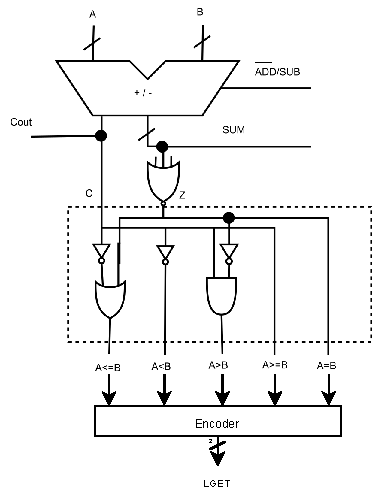
\includegraphics[width=0.3\textwidth]{chapters/4_DecodeStage/images/cmp_final.pdf}
	\caption{Final implementation of the comparator}
	\label{cmp_final}
\end{figure}

\section{Jump and Branch decision}
\section{Next Program Counter computation}
\chapter{Execute Stage}

\begin{figure}[ht]
	\centering
	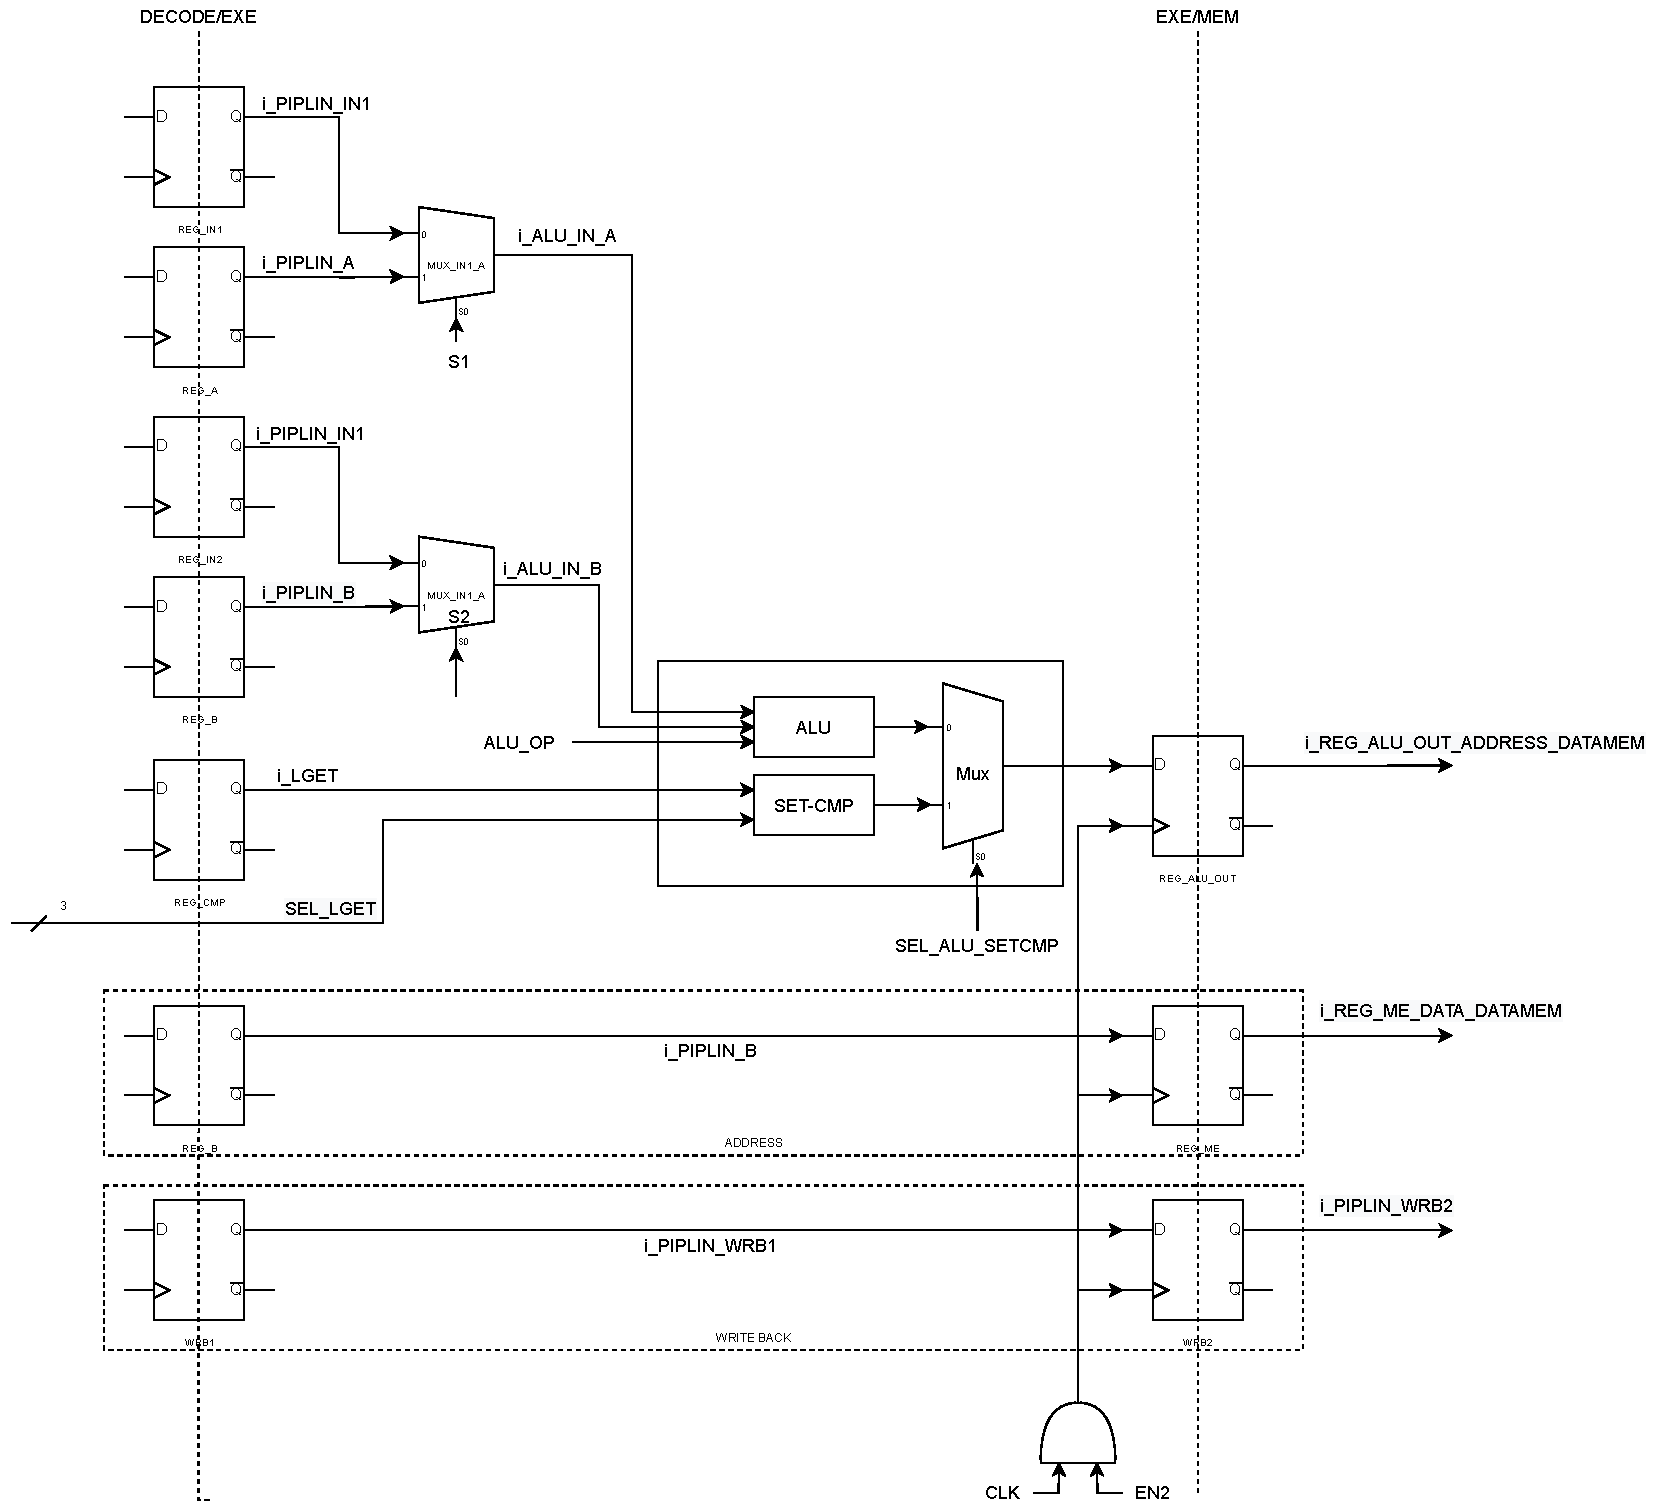
\includegraphics[width=0.8\textwidth]{chapters/5_ExecuteStage/images/exe_stage.pdf}
	\caption{Execute stage}
	\label{fig:execute-stage}
\end{figure}

\section{ALU: Arithmetic Logic Unit}
\begin{figure}[h]
	\centering
	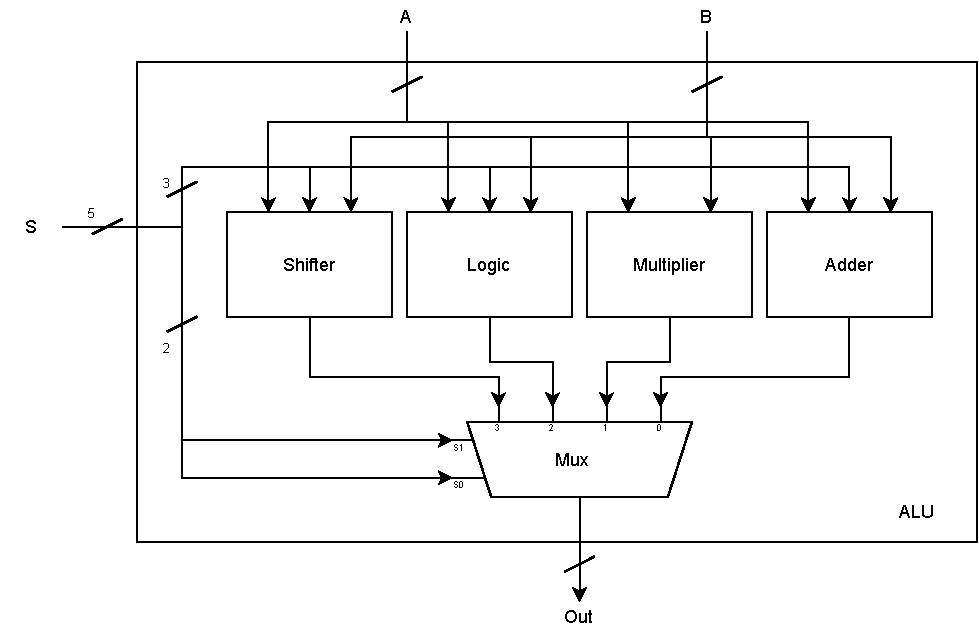
\includegraphics[width=0.7\textwidth]{chapters/5_ExecuteStage/images/ALU.pdf}
	\caption{ALU unit}
	\label{fig:ALU}
\end{figure}
The Arithmetic Logic Unit can be seen as a block, that given a selection signal and the inputs is able to perform computation over the operands. The ALU implementation described in this document is based on the following block:
\begin{itemize}
	\itemsep0sp
	\item Adder
	\item Multiplier
	\item Logic unit
	\item Shifter
\end{itemize}
Each one of these blocks will be explained in the following sections.


The base concept is that, internally, the 4 units are selected through a multiplexer that takes two out five bits from a selection signal called \texttt{OP}. Having 5 bits to describe the type of operation, the possible combinations and their relative operations are:
\begin{table}[H]
	\centering
	\begin{tabular}{c | l}
		\texttt{LGET} & \textbf{Description}\\
		\hline
	
	\end{tabular}
	\caption{LGET encoding}
\end{table}

The two LSBs are the ones used as selection input for the multiplexer that select from which ALU unit takes the result. In fact, the univocally define the unit to be used. The remaining three MSBs are used as input for the units that compose the ALU in order to select the correct operation.

\subsection{Adder}
The straightforward way to implement an adder is to use the Ripple Carry Adder structure, that is composed of $N-1$ Full Adder and one Half Adder (the first), where $N$ is the number of bits of the two operands. This solution is not optimal from a timing point of view due to the time needed to propagate the carry, that defines the critical path, that is the bottleneck. \newline\newline
Since the sum and the subtraction is one of the most common operation, the DLX includes an adder that is based on a CLA - Carry Look Ahead (Sparse Tree) and a Carry Select Like Adder. The complete structure can be seen at figure \ref{fig:P4}.

\begin{figure}[h]
	\centering
	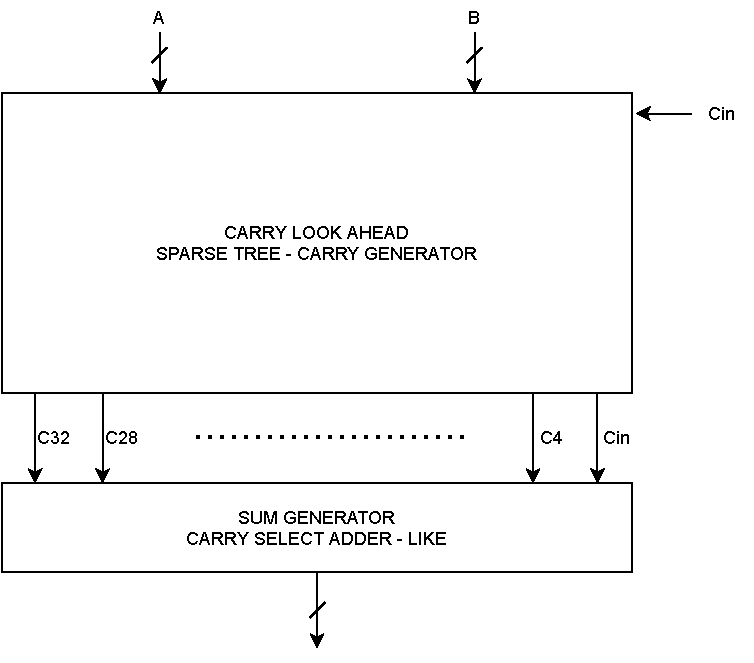
\includegraphics[width=0.5\textwidth]{chapters/5_ExecuteStage/images/P4.pdf}
	\caption{Booth's multiplier on 32 bits}
	\label{fig:P4}
\end{figure}
As said before, the adder is composed of two blocks:
\begin{itemize} 
	\item \textbf{Carry Select Like Adder}: The main point of the Carry Select Adder is that it doubles the complexity of the adder itself in order to obtain better performances. It is composed by two RCA, in order to perform two sums in parallel.
	
	The idea is to compute both the results, on 4 bits in this case, for both when the carry-in is equal to `0' or `1'. In this way, the results is computed in parallel for all the stages, even if the carry-in is `0' or `1'; then the carry-in is used to mux against the two results (on 4 bits) and the two carry-outs. The carry-out will be used as result selection signal for the next Carry Select unit.
	
	We are paying complexity in order to reduce the addition computation time, in fact by having a carry out that is used as carry in for the next state, there is still propagation but is lower.\newline\newline	
	The DLX implementation, instead of using a straightforward implementation of the Carry Select Adder, it uses a modified version of it. It has been implemented using \textit{CLA - Sparse Tree Carry Generator} and a \textit{Carry Select Like Adder}. The base idea is to use the CLA in order to compute a carry every $n$ bits, then these carries are fed into the sum generator that uses them to compute the results in parallel.
	\begin{figure}[H]
		\centering
		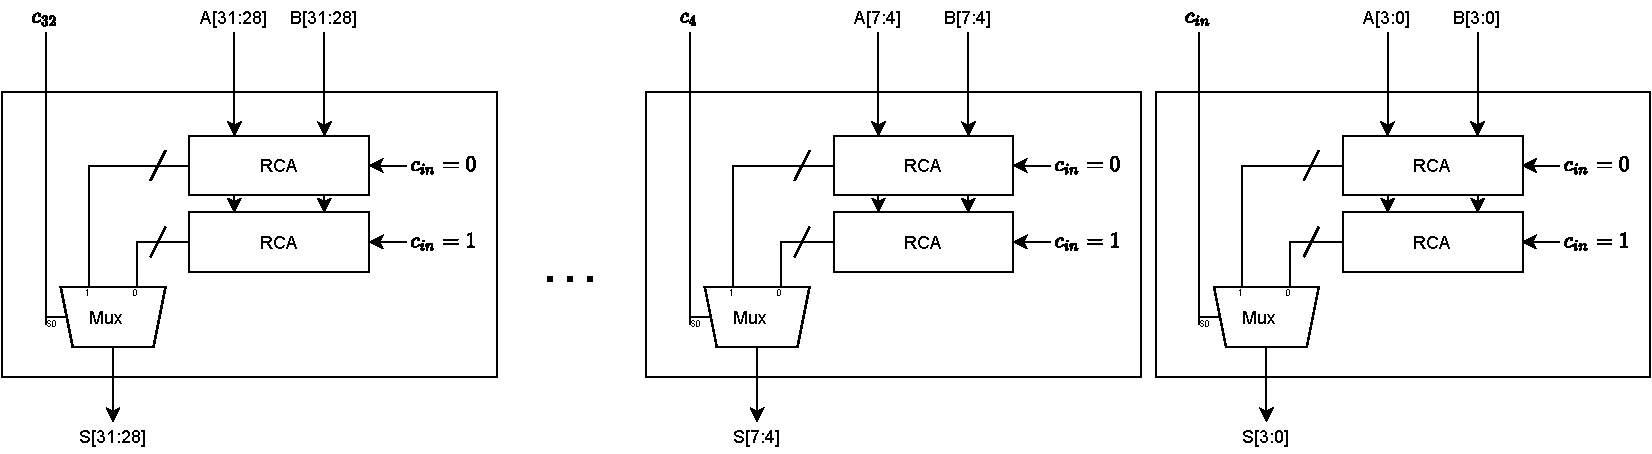
\includegraphics[width=1\textwidth]{chapters/5_ExecuteStage/images/carry_sum.pdf}
		\caption{Carry Select Like Adder block for a 32 bits implementation}
		\label{fig:carry_sum}
	\end{figure}
	\item \textbf{Carry Look Ahead - Sparse Tree}: this block is used to compute the carry out every 4 bits. The idea behind the CLA is to compute several carries simultaneously and to avoid waiting until the correct carry propagates from the stage of the adder in which it has been generated. This is done thanks to the \textit{propagate (P)} (that is 1 if the carry-in is equal to the carry-out) and \textit{generate (G)} (that is one if carry-in is 0 and carry-out is 1).
	\begin{table}[H]
		\begin{center}
			\begin{tabular}{ c c c | c c | c c}
				$a$ & $b$ & $c_{in}$ & $out$ & $c_{out}$ & $p$ & $g$ \\
				\hline
				0 & 0 & 0 & 0 & 0 & 0 & 0\\ 
				0 & 0 & 1 & 1 & 0 & 0 & 0\\ 
				0 & 1 & 0 & 1 & 0 & 1 & 0\\ 
				0 & 1 & 1 & 0 & 1 & 1 & 0\\ 
				1 & 0 & 0 & 1 & 0 & 1 & 0\\ 
				1 & 0 & 1 & 0 & 1 & 1 & 0\\ 
				1 & 1 & 0 & 0 & 1 & 0 & 1\\ 
				1 & 1 & 1 & 1 & 1 & 0 & 1\\ 
			\end{tabular}
			\caption{Computation of propagate and generate bits}
		\end{center}
	\end{table}
	\begin{equation} \label{eq:pandg}
		g = a \oplus b \quad\quad p = a \cdot b
	\end{equation}
	The base idea is to write any $s_i$, that is the i-esim bit of the sum and $c_i$, the carry-out at $i$ index in function of $p$ and $g$.
	We now use $p$ and $g$ to express the same result:
	\begin{align*}
		& s_1 = a \oplus b \oplus c_{in} = p_1 \oplus c_0\\
		& c_1 = a \cdot b + a \cdot c + b \cdot c = a_1 \cdot b_1 + (a_1 + b_1) \cdot c_0 =  g_1 + p_1 \cdot c_0
	\end{align*}
	The crucial point is that it's possible to compute the carry at $i$ position only using the initial carry-in $c_{in}$ and $p$ and $g$ generate in the current and previous blocks. Tree are a family of Carry Look Ahead that differ for the carry-logic. They are based always on \textit{propagate} and \textit{generate}. We have that 	
	\begin{align*}
		& carry = g + p \cdot c_{in}\\
		& G_{i:j} = G_{i:k} + P_{i:k} \cdot G_{k-1:j}\\
		& P_{i:j} = P_{i:k} \cdot P_{k-1:j}
	\end{align*}
	where
	\begin{itemize}
		\itemsep0sp
		\item $i \ge k > j$
		\item $G_{x:x} = g_x$ and $P_{x:x} = p_x$
		\item $g_0 = C_{in}$
	\end{itemize}
	The white and gray blocks in the Sparse Tree block at \ref{fig:pg_network}, that are used in the \texttt{carry\_generator} block, are PG and G blocks.
	Normally two blocks are used, the first \textit{G} generates only $G_{i:j}$ and the other \textit{PG} both $G_{i:j}$ and $P_{i:j}$.
	\begin{figure}[h]
		\centering
		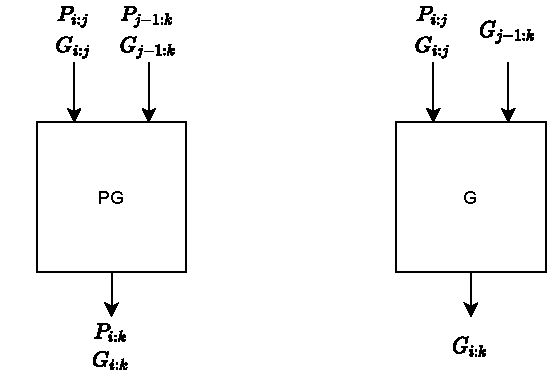
\includegraphics[width=0.4\textwidth]{chapters/5_ExecuteStage/images/PG_and_G.pdf}
		\caption{PG and P block}
		\label{fig:PG_and_G}
	\end{figure}
	The base idea is to combine their outputs and take only the G one as carries.
\end{itemize}
So, Carry Look Ahead - Sparse Tree needs a starting block that generates all the $p$ and $g$ for all the couples of bit using the \ref{eq:pandg} equation. The spars tree and the PG network structure is shown in the figure \ref{fig:pg_network}, in the code this block is called \texttt{prop\_gen\_generic} and is made of \texttt{prop\_gen} block in order to compute $p$ and $g$.
\begin{figure}[H]
	\centering
	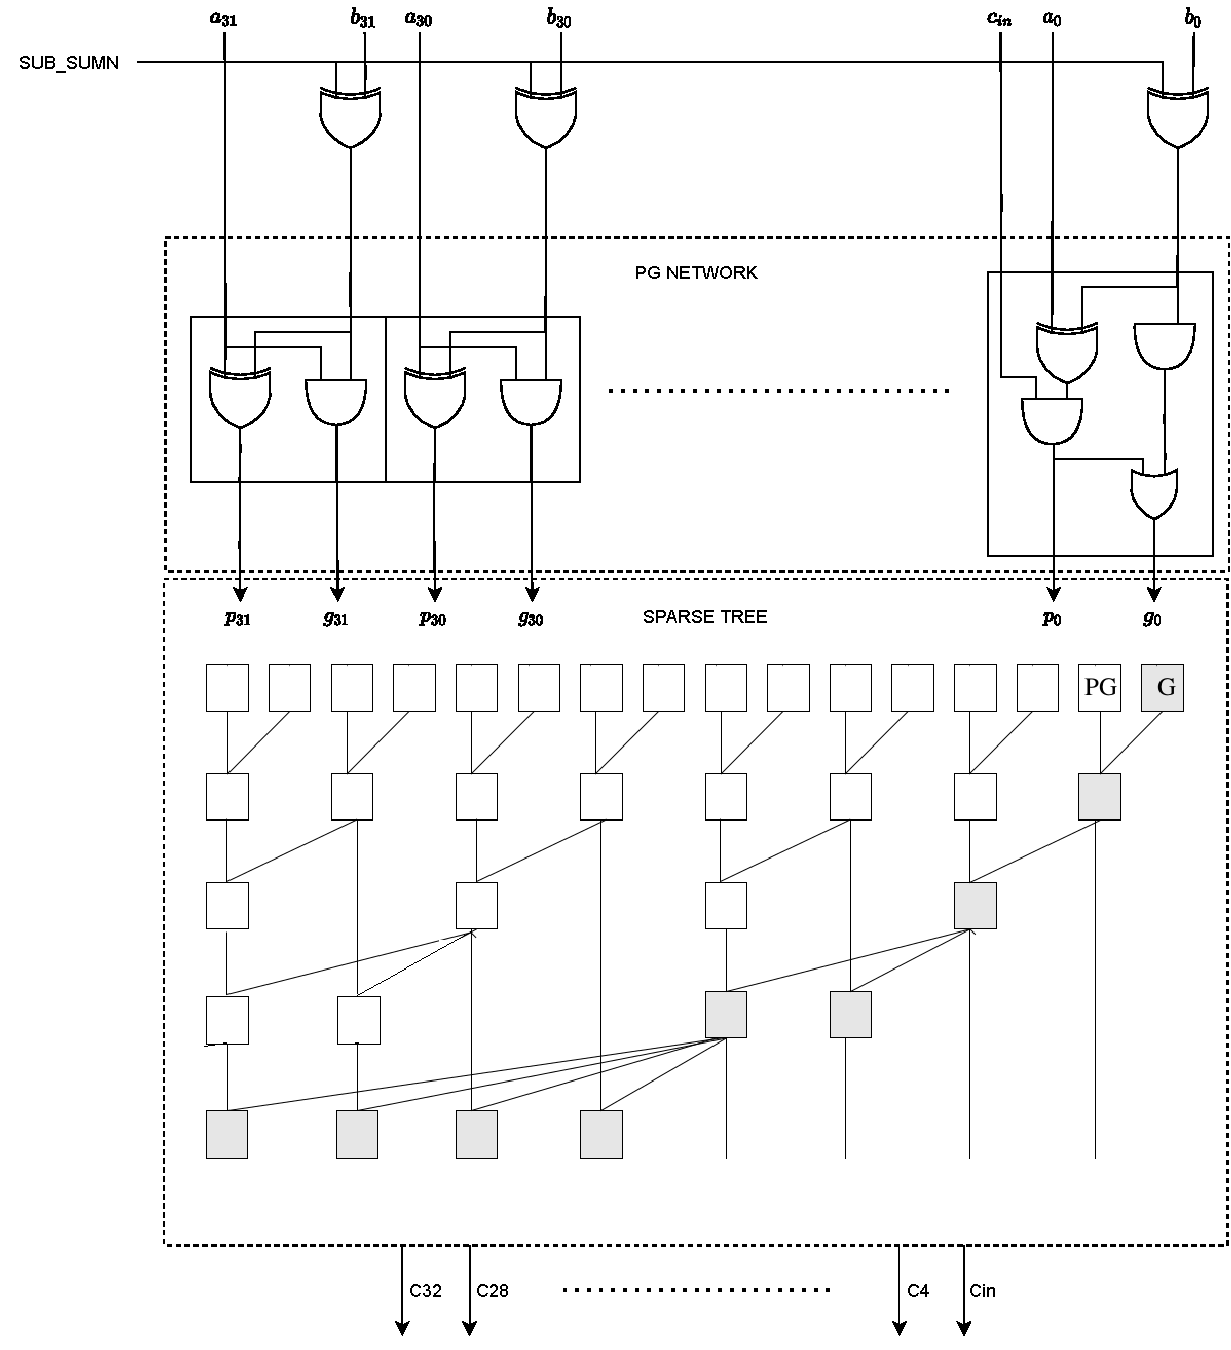
\includegraphics[width=0.7\textwidth]{chapters/5_ExecuteStage/images/CLA.pdf}
	\caption{Carry Look Ahead - Carry Generator Block}
	\label{fig:pg_network}
\end{figure}
In order to be able to perform both subtraction and sum, the first block must be modified and must include the logic to manage also the carry-in, that in case of a subtraction it is `1'. This is not enough to perform subtraction, in fact, an additional signal called \texttt{SUB\_SUMN} is needed.
So, the same structure can be used to implement the subtraction, by adding an XOR on each B input with the \texttt{SUB\_SUMN} control signal.

We can say that a subtraction in 2's complement can be implemented as $A + \overline{B} + 1$; in order to implement this in the circuit we need to set the carry-in to `1' (so \texttt{SUB\_SUMN} = `1') in order to add 1 and invert the B input by using the XOR. In fact:
\begin{displaymath}
	\begin{array}{c c|c}
		% |c c|c| means that there are three columns in the table and
		% a vertical bar '|' will be printed on the left and right borders,
		% and between the second and the third columns.
		% The letter 'c' means the value will be centered within the column,
		% letter 'l', left-aligned, and 'r', right-aligned.
		x & y & y \oplus q\\ % Use & to separate the columns
		\hline % Put a horizontal line between the table header and the rest.
		0 & 0 & 0\\
		0 & 1 & 1\\
		1 & 0 & 1\\
		1 & 1 & 0\\
	\end{array}
\end{displaymath}
This solution is good because the PG and G block has the same delay, that is driven by G and since both include it, they are the same. Many paths have the same delay and the load on components is good since an output of a block is connected at maximum to 2 other block. These two factors bring a good \textit{equilibrium} to the entire structure.
\subsection{Multiplier}
In order to overcome the limitation of the array multiplier, this DLX implementation includes a modified version of the Booth's multiplier, since the multiplex for the partial values to be added is only on two bits instead of three. The Booth's algorithm copes with 3 bits at a time, so the number of stages is $N/2$ (this corresponds to the number of the encoders) and this allows to speed up the result computation. 
The Booth's algorithm is the following:
\begin{lstlisting}[frame=none, escapeinside={(*}{*)}]
	i = 0
	P = 0
	while i (*$\leq$*) M - 2 loop
		P = P + Vp( (*$B_{i+1}, B_i, B_{i-1}$*) )
		A = A * 4
		i = i + 2
	end loop
\end{lstlisting}
Where \texttt{P} is the final value of the product and during the algorithm execution it will contain the partial result; \texttt{M} represents the number of bit of the multiplicand, in this case $B$. The algorithm takes as convention that $B_{i-1} = 0$. The \texttt{Vp} is a lookup table (see \ref{mult:lut}), that return the value to add to \texttt{P}, according to the 3 bits selected. The value of $A$ is multiplied by 4.

\begin{table}[H]
	\begin{center}
		\begin{tabular}{ c c c | c}
			$B_{i+1}$ & $B_{i}$ & $B_{i-1}$ & \\
			\hline 
			0 & 0 & 0 & 0\\ 
			0 & 0 & 1 & +A\\ 
			0 & 1 & 0 & +A\\ 
			0 & 1 & 1 & +2A\\ 
			1 & 0 & 0 & -2A\\ 
			1 & 0 & 1 & -A\\ 
			1 & 1 & 0 & -A\\ 
			1 & 1 & 1 & 0\\ 
		\end{tabular}
		\caption{Booth's LUT}
		\label{mult:lut}
	\end{center}
\end{table}

The Booth's multiplier work with 3 main components, supposing $A$ is the multiplicand and $B$ the multiplier:
\begin{enumerate}
	\item $N/2$ encoders in order to take 3 bits from the operand $B$; the two LSB are used as selection signal for the multiplexers and the last one, the MSB, for the adder. In fact, as it's possible to notice from the table \ref{mult:lut}, when the MSB is 1 the value to be added to the partial result is positive, negative otherwise. For this reason, the inputs to the multiplexers are only $\{0, A, 2A\}$. Since we need also to generate negative values, like ${-A, -2A}$, the MSB of the three bits is used as input for the adder. This signal, called \texttt{SUB\_SUMn} is used to define if the operation is a sum or a subtraction; if it is 1, a subtraction is performed;
	\item $N/2$ multiplexers that select only among $\{0, A, 2A\}$, since at each stage $A$ must be multiplied by 4, a shift by two is done starting from $A$ of the previous multiplexer;
	\item $N/2$ ripple carry adders, that allow to preform the partial sums. Since the final results will be on $NBIT \cdot 2+1$ bits, the adders in each level have been optimized in order to work only with the minimum bits needed. In fact, the adder at $i$ level, will generate the result on $NBIT + 2 \cdot i$ bits. As said before, an addition signal called \texttt{SUB\_SUMn} has been added in order to be able to perform the subtraction. The Ripple Carry Adder has been select for its simplicity and since the multiplication is a less common instruction, it was not worth to use a more sophisticated adder. This allowed to reduce the total area of the multiplier itself.
\end{enumerate}
The multiplexer implements the \textit{LUT} and at the same time the $A = A \cdot 4$. The two values from the two multiplexer are summed together via an adder, this implements the partial sum. The overall structure can be observed at \ref{fig:multiplier}.

\begin{figure}[ht]
	\centering
	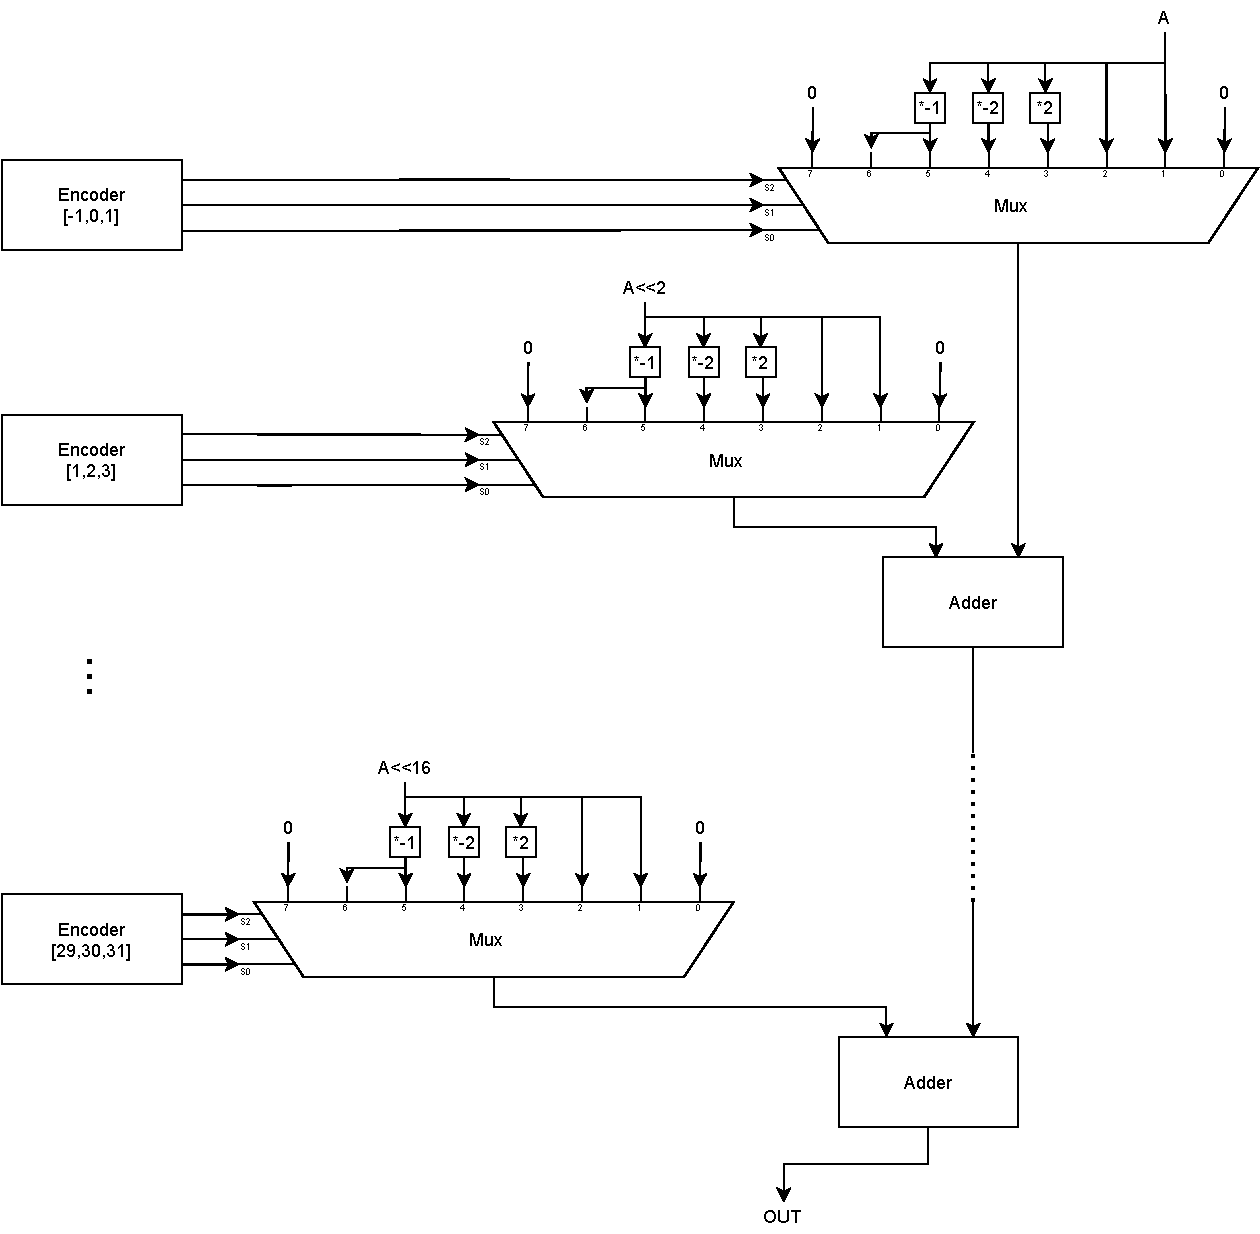
\includegraphics[width=0.8\textwidth]{chapters/5_ExecuteStage/images/multiplier.pdf}
	\caption{Booth's multiplier on 32 bits}
	\label{fig:multiplier}
\end{figure}

	
\subsection{Logic Operands}
The basic and most simple implementation of a logic unit is based on single logic gates on $N$ bits whose outputs are muxed, in order to generate the correct output. The problem with this solution is that the number of input signals to the multiplexer is extremely high; this implementation does not only suffer from the point of view of the delay but, since each logic function is implemented with a specific gate, the total area is huge.\newline\newline
In order to overcome the problems highlighted before, a more compact implementation has been chosen: the T2 logic unit.

This logic unit allows to perform AND, NAND, OR, NOR, XOR and XNOR using only 5 NAND gates, on two levels, and 4 selection signals. The schematic is the one in figure \ref{fig:log_unit}.

\begin{figure}
	\centering
	\tikzstyle{branch}=[fill,shape=circle,minimum size=3pt,inner sep=0pt]
	\begin{tikzpicture}[label distance=2mm]
		\draw (0.92,-0.40) -- (1.09,-0.56);
		\draw (1.92,-0.40) -- (2.09,-0.56);
		% nodes
		\node (y1) at (1,0) {$R_1$};
		\node (y2) at (2,0) {$R_2$};
		\node[not gate US, draw, rotate=-90] at ($(y1)+(0.5,-1.5)$) (noty1) {};
		\node[not gate US, draw, rotate=-90] at ($(y2)+(0.5,-1.5)$) (noty2) {};
		
		% draw nodes to NOT
		\foreach \i in {1,2} {
			\path (y\i) -- coordinate (punt\i) (y\i |- noty\i.input);
			\draw (punt\i) node[branch] {} -| (noty\i.input);
		}
	
		\node (x1) at (0,-2.33) {$S_0$};
		\node (x2) at (0,-3.33) {$S_1$};
		\node (x3) at (0,-4.33) {$S_2$};
		\node (x4) at (0,-5.33) {$S_3$};
		
		\node[nand gate US, draw, logic gate inputs=nnn] at ($(y2)+(2,-2.5)$) (And1) {};
		\node[nand gate US, draw, logic gate inputs=nnn] at ($(And1)+(0,-1)$) (And2) {};
		\node[nand gate US, draw, logic gate inputs=nnn] at ($(And2)+(0,-1)$) (And3) {};
		\node[nand gate US, draw, logic gate inputs=nnn] at ($(And3)+(0,-1)$) (And4) {};
		\node[nand gate US, draw, logic gate inputs=nnnn, anchor=input 1] at ($(And1.output -| And2.output)+(2,-1.25)$) (Or1) {};
		

		% connect x_i to AND_i
		\foreach \i in {1,2,3,4} {
			\draw (x\i) -- (And\i.input 1);
		}
		
		% y1

		\draw (noty1 |- And1.input 2) node[branch] {} -- (And1.input 2);
		\draw (noty1 |- And2.input 2) node[branch] {} -- (And2.input 2);
		\draw (y1 |- And3.input 2) node[branch] {} -- (And3.input 2);
		\draw (y1) |- (And4.input 2);
		\draw (noty1) |- (And2.input 2);
		
		\draw (noty2 |- And1.input 3) node[branch] {} -- (And1.input 3);
		\draw (y2 |- And2.input 3) node[branch] {} -- (And2.input 3);
		\draw (noty2 |- And3.input 3) node[branch] {} -- (And3.input 3);
		\draw (y2) |- (And4.input 3);
		\draw (noty2) |- (And3.input 3);
		

		% AND
		\draw (And1.output) -- ([xshift=0.8cm]And1.output) |- (Or1.input 1);
		\draw (And2.output) -- ([xshift=0.6cm]And2.output) |- (Or1.input 2);
		\draw (And3.output) -- ([xshift=0.6cm]And3.output) |- (Or1.input 3);
		\draw (And4.output) -- ([xshift=0.8cm]And4.output) |- (Or1.input 4);
	
		
		% OR
		\draw (Or1.output) -- ([xshift=0.5cm]Or1.output) node[above] {$out$};
		
	\end{tikzpicture}  
	\caption{Logic unit}
	\label{fig:log_unit}
	\end{figure}

	In order to compute one of the logical instructions, the select signals are properly activated as follow:
	
	\begin{figure}[ht]
		\centering
	\[
	\begin{vmatrix}
		S_0 & S_1 & S_2 & S_3 & \text{Operation}\\
		0 & 0 & 0 & 1 & AND \\
		1 & 1 & 1 & 0 & NAND \\
		0 & 1 & 1 & 1 & OR \\
		1 & 0 & 0 & 0 & NOR \\
		0 & 1 & 1 & 0 & XOR \\
		1 & 0 & 0 & 1 & NXOR \\
	\end{vmatrix}
	\]
	  \caption{Logic input signals with the relative operation}
	  \label{tab:log_sign}
\end{figure}
	
	For example, in order to generate the AND logical operation, we have to select $S_3 = 1$, so that $out = R_1 \cdot R_2$; on the other hand, if we need NAND $S_0 = S_1 = S_2 = 1$ and $S_3 = 0$, so that $out = \overline{R_1} \cdot \overline{R_2} + \overline{R_1} \cdot R_2 + R_1 \cdot \overline{R_2} = \overline{R_1} \cdot \overline{R_2}$ that using the De Morgan law $out = \overline{R_1 \cdot R_2}$.
	This allows to obtain the best performances also because all paths work in parallel, compacting the area and the delay.\newline\newline
	Since only the 3 bits are used to select among the logical operations (\texttt{S} signal), a direct correspondance is needed to generate the signal show in table \ref{tab:log_sign}. The following table, shows the conversion:
	\begin{table}[H]
		\begin{center}
			\begin{tabular}{ c| c}
				\texttt{S} & Decoded signal \\
				\hline
				000 & 0001 \\
				001 & 1110 \\
				010 & 0111 \\
				011 & 1000 \\
				100 & 0110 \\ 
				101 & 1001 \\ 
				110 & 0000 \\ 
				
			\end{tabular}
			\caption{Conversion table, from \texttt{S} input signal on 3 bits into 4 bits}
		\end{center}
	\end{table}

\subsection{Shifter}
The implemented shifter allows to perform shift right, logical/arithmetical shift left and left/right rotate using the full operand \texttt{A} on 32 bits and 6 bits from the second one \texttt{B} and three \textit{control signals}.
Differently from the T2 version, it uses and addition signal in order to be able to manage also the rotate instruction. Our implementation takes three inputs:
\begin{itemize}
	\itemsep0sp
	\item \texttt{A}: the operand to be shifted/rotated;
	\item \texttt{B}: only the 5 LSB [4,3,2,1,0] are used to select first the mask to be used and then the starting point from that mask;
	\item \texttt{SEL}: it encodes the operation type; the second bit is used to select among arithmetic and logic, the third bit is used to select the direction of the shift/rotate (left/right) and the first one is used only if the operation is a rotate. This is the encoding:
	\begin{center}
		\begin{tabular}{c|l}
			\texttt{SEL} & \textbf{Operation}\\
			\hline
			000 & Shift logic right \\
			001 & Shift logic left \\
			010 & Shift arith right \\
			011 & Shift arith left \\
			100 & Rotate right \\
			101 & Shift right \\
		\end{tabular}
	\end{center}
\end{itemize}

\begin{figure}[ht]
	\centering
	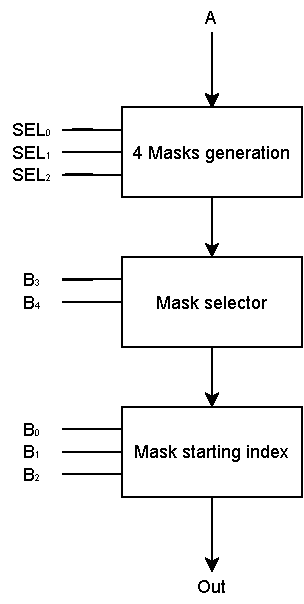
\includegraphics[width=0.2\textwidth]{chapters/5_ExecuteStage/images/Shifter.pdf}
	\caption{Blocks of the Shifter/Rotate Unit}
	\label{fig:shifter}
\end{figure}

 The unit perform the requested operation in three stages, sketched in figure \ref{fig:shifter}:
\begin{enumerate}
	\item The first consist in preparing 4 possible ``masks", each already shifted of {0, 8, 16, 32} left
	or right depending on the configuration. This allows to shift for all 32 bits. Basically it copies
	the input \texttt{A} into the 4 masks that will be used by the next stage. Being in 32 bits, the generated masks are in $32+8=40$ bits. The only different between this implementation and the T2 one, is that, in case of rotate, the additional 8 bits of the masks are filled with the corresponding 8 bits that are going ``out" during the rotation.
	
	\item The second level perform a coarse grain shift, that is basically consist on selecting one mask
	among the 4 possible masks generated in the previous stage. This selection is done by using the bits {4, 3} of \texttt{B}.
	\item The third level, using the bits {2, 1, 0} of \texttt{B} and the selected mask, preform a fine grain refinement. The 3 bits allows to select the starting index from the mask, in fact it allows to select among 8 positions.
\end{enumerate}



\begin{figure}[h] 
	\label{ fig7} 
	\begin{minipage}[b]{0.5\linewidth}
		\centering
		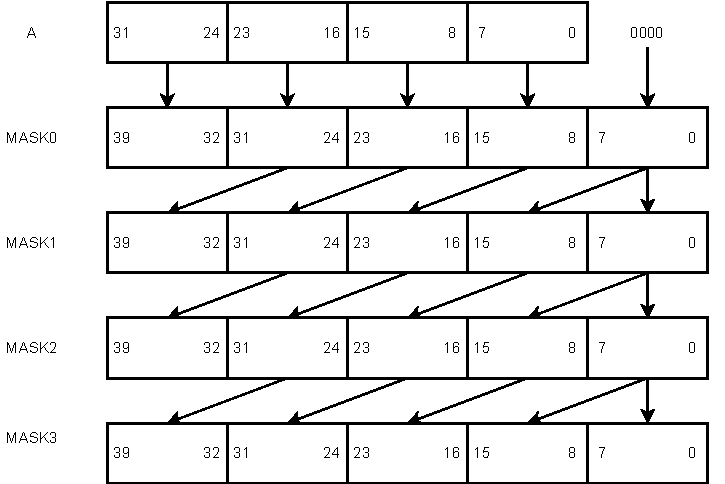
\includegraphics[width=.78\linewidth]{chapters/5_ExecuteStage/images/left_shift.pdf} 
		\caption{Masks for left shift} 
		\vspace{4ex}
	\end{minipage}%%
	\begin{minipage}[b]{0.5\linewidth}
		\centering
		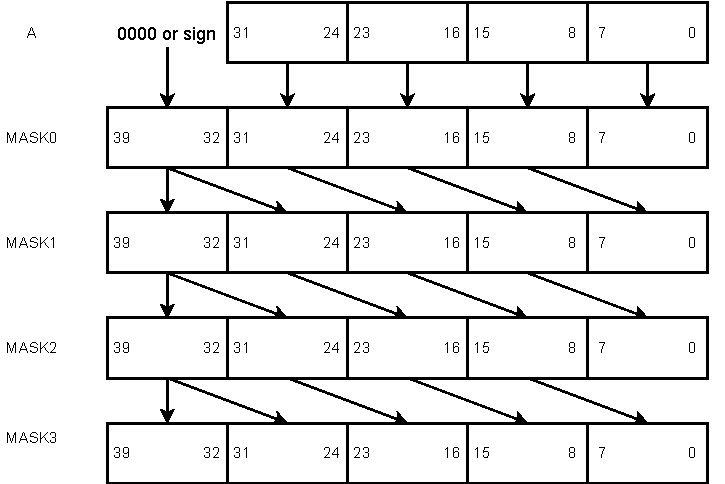
\includegraphics[width=.78\linewidth]{chapters/5_ExecuteStage/images/right_shift.pdf}
		\caption{Masks for right shift} 
		\vspace{4ex}
	\end{minipage} 
	\begin{minipage}[b]{0.5\linewidth}
		\centering
		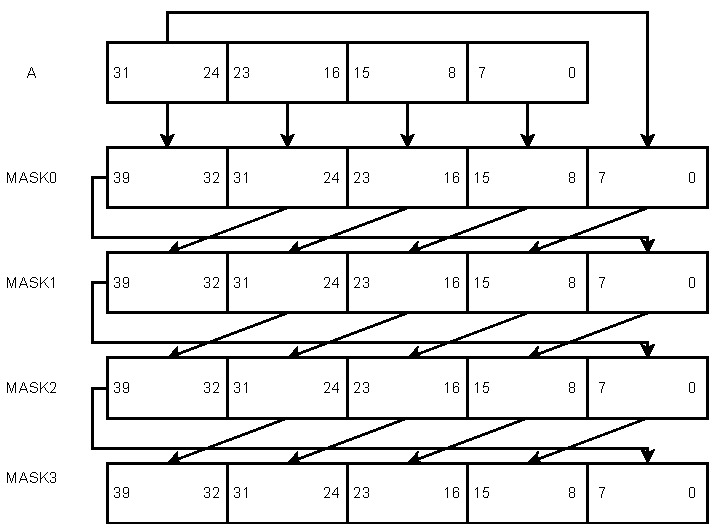
\includegraphics[width=.78\linewidth]{chapters/5_ExecuteStage/images/left_rotate.pdf} 
		\caption{Masks for left rotate} 
		\vspace{4ex}
	\end{minipage}%% 
	\begin{minipage}[b]{0.5\linewidth}
		\centering
		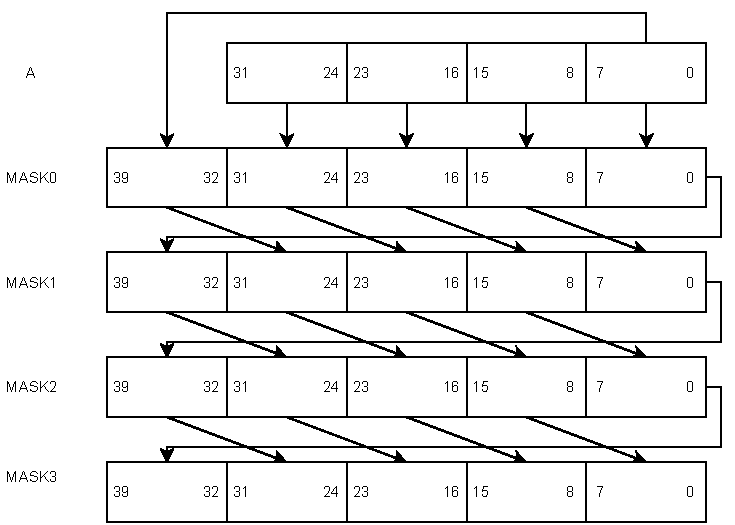
\includegraphics[width=.78\linewidth]{chapters/5_ExecuteStage/images/right_rotate.pdf} 
		\caption{Masks for right rotate} 
		\vspace{4ex}
	\end{minipage} 
	\caption{Masks for shift unit on 32 bits} 
\end{figure}
\begin{mybox}
	\textbf{Examples}
	\newline
	For example, if we need to perform a left left of 9 bits \texttt{A}, where \texttt{A=18}, the corresponding \texttt{B} value will be 1001; this means that the second masks will be taken and the output result will from the bit at position $40-1=39$ to the one at $39-32=7$ included.
	\begin{center}
		MASK 2: 0$\underbrace{\textbf{0000000 00000000 00000000 00010010 0}}_{\text{shifted \texttt{A}}}$0000000
	\end{center}
	
	On the other hand, if we need to perform a right shift the masks are generated in the opposite way, so the zeros are put in the MSB of the mask, shifted by 0, 8 ... positions. In this case we need also to distinguish between the an arithmetic and a logic shift; in the first case, instead of filling the ``empty" bits with zero, the operand sign is used. For example, if we want to shift \texttt{A=-18} of \texttt{B=3} bits, the first mask is used: 
	\begin{center}
		MASK 1: 11111$\underbrace{\textbf{111 11111111 11111111 11111111 11101}}_{\text{shifted \texttt{A}}}$110
	\end{center}
	
	In the last case, let's suppose to rotate right \texttt{A=1255} (=10011100111) by 5 position:
	\begin{center}
		MASK 1: 11$\underbrace{\textbf{100111 00000000 00000000 0000100 111}}_{\text{rotated \texttt{A}}}$00111
	\end{center}
	As you can see, in case of MASK 1 for the right rotation, the 8 LSB of \texttt{A} are copied into the 8 MSB of the mask.
\end{mybox}
	

\section{Set-Like Operations Unit}

\begin{figure}[ht]
	\centering
	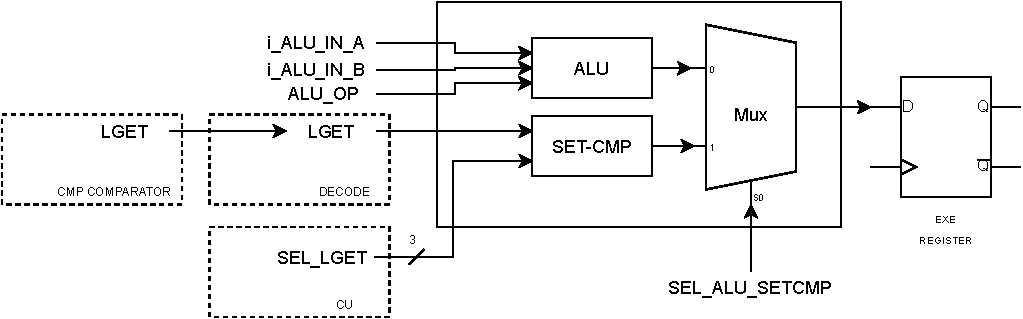
\includegraphics[width=0.8\textwidth]{chapters/5_ExecuteStage/images/set_cmp.pdf}
	\caption{Execute stage with focus on the SET-CMP unit}
	\label{fig:set-cmp}
\end{figure}

The DLX execution stage includes also the possibility to set the value of a register accordingly to the outcome of the comparison of two operands; the operands can came from two sources:
\begin{enumerate}
	\item Both from the register file, trough \texttt{REG\_B} and \texttt{REG\_A} (refer to figure \ref{fig:execute-stage});
	\item One from the register file (\texttt{REG\_A} by setting \texttt{S1 = 0}) and the immediate from \texttt{REG\_IN2} (refer to figure \ref{fig:execute-stage}).
\end{enumerate}

The unit designed to perform this set operation is called \texttt{set\_comparator}, that using a behavioural process, is able to generate the corresponding `1' or `0' to be set to the register, accordingly to the comparison result. The output on $N BIT_DATA$ bits will be muxed with the one coming from the ALU unit, using the CW that is configured in the Control Unit.

In order to decrease the area and since the comparison was already generated by the comparator unit in the decode stage (refer to section \ref{sec:comparator}), the \texttt{set\_comparator} unit takes the \texttt{LGET} signal that came from the decode unit and perform the following checks:

\begin{table}[H]
	\begin{center}
		\begin{tabular}{ c | l}
			\textbf{Operation} & \textbf{VHDL implementation} \\
			\hline
			\texttt{SEQ} & \texttt{not LGET(0)} \\
			\texttt{SNE} & \texttt{LGET(0)} \\
			\texttt{SLE} & \texttt{LGET(1) = `0' or LGET(0) = `0'} \\
			\texttt{SLT} & \texttt{LGET = "01"} \\
			\texttt{SGE} & \texttt{LGET(1) = `1' or LGET(0) = `0'} \\
			\texttt{SGT} & \texttt{LGET = "11"}
			
		\end{tabular}
		\caption{Performed checks in order to generate `1' or `0' accordingly to the comparison outcome. Refer to table \ref{tab:lget}.}
	\end{center}
\end{table}



\chapter{Memory Stage}
\label{chp:memory_stage}
The memory stage allows to perform operations with the memory, the DRAM in this case, in order to load or store a value from/to the memory respectively. Figure \ref{fig:mem_stage} shows the Memory Stage of the DLX pipeline.

\begin{figure}[H]   
    \centering
    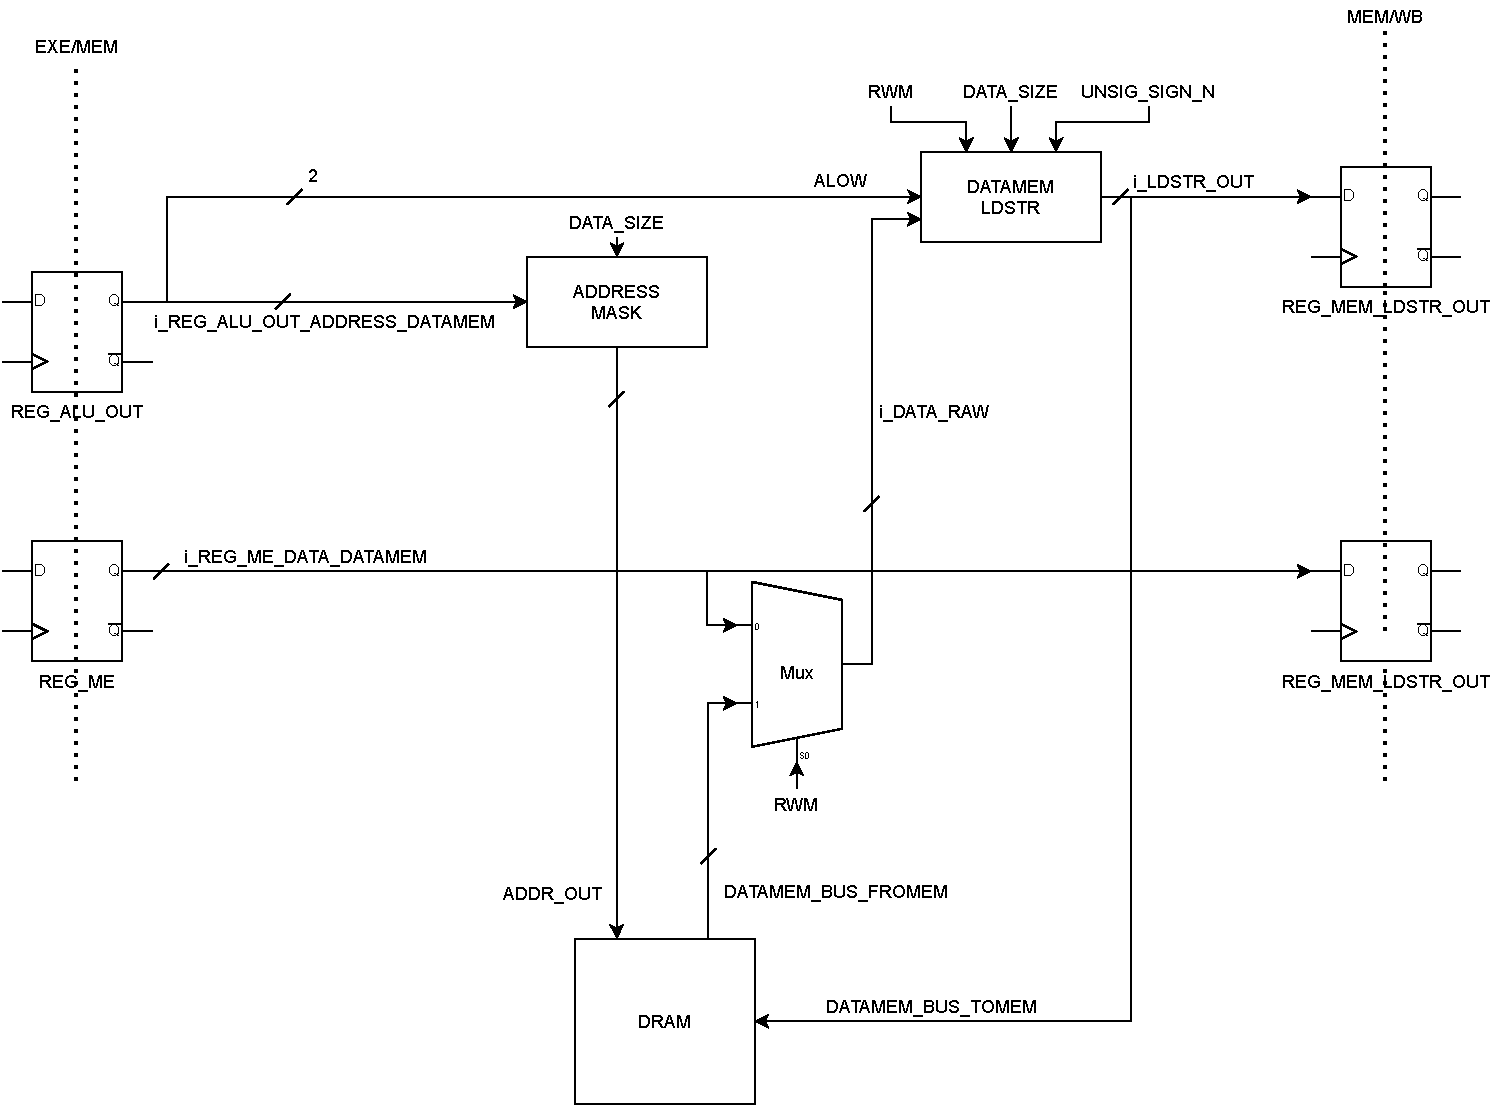
\includegraphics[width=0.85\textwidth]{chapters/6_MemoryStage/images/mem_stage.pdf}
    \caption{Memory stage}
    \label{fig:mem_stage}
\end{figure}

If the instruction that reaches the memory stage is a load, the value stored into the \texttt{REG\_ALU\_OUT} register is fed to a block that performs the masking of the address itself. Then the masked address is given as input to the external memory in order to retrieve the data. A multiplexer with two inputs allows to select the data coming from the memory and redirects it to another unit, called \texttt{datamem\_ldstr} that uses the \texttt{DATA\_SIZE} and \texttt{UNSIG\_SIGN\_N} inputs to select the correct bits for word, half-word and byte.

In the case of a store, the address in which the data must be saved into the memory is masked too via the Address Mask Unit and its output is given to the DRAM. The data stored in the \texttt{REG\_ME} register is selected, by correctly configuring the multiplex to choose it, and put as input to the \texttt{datamem\_ldstr} unit. The output of this unit is put as input data to the DRAM, that performs the store.

\section{Address Mask Unit}
The basic idea behind the Address Mask Unit is to modify the address, given as input, depending on the data size to store or load. All the possibility and masking procedures are summed up in Table \ref{tab:addr_masking}. 

\begin{table}[ht]
    \begin{center}
        \begin{tabular}{ c| l | l}
            \texttt{DATA\_SIZE} & \textbf{Dimension} & \textbf{Masking}\\
            \hline
            00 & word & \texttt{ADDR\_IN(ADDR\_IN'length-1 downto 2) \& "00"}\\
            01 & half word & \texttt{ADDR\_IN(ADDR\_IN'length-1 downto 1) \& "0"} \\
            10 & byte & \texttt{ADDR\_IN}
            
        \end{tabular}
        \caption{Address masking for all the three possible cases}
        \label{tab:addr_masking}
    \end{center}
\end{table}


Give an address, it must be correctly aligned depending on the dimension of the data the processor want to write/read to/from memory. Refer to the \ref{vhdl_masking_addr} VHDL snippet. The problem with the alignment arises when data to be accessed are larger than the addressable unit (word vs byte). \\

After the generation of the correct address, is a DRAM duty to output the data in the proper byte lanes, as explained in Table \ref{table:memory_read_configuration}. The operation of reading from the correct byte lane and apply a sign extension (if requested) is made by the \ref{sec:ldstr} \emph{Load-Store Unit}.

% This allows to read always 32 bits from the memory from the correct position, thanks to the masking process. Since the data is on 32 bits, we need to select 8, 16 or 32 bits from it accordingly to the \texttt{DATA\_SIZE} two bits signal. This is done in the Load-Store Unit.


\hfill
\begin{lstlisting}[style=vhdl,caption={VHDL code for address alignment},label=vhdl_masking_addr]
    with DATA_SIZE select
        ADDR_OUT <= ADDR_IN(ADDR_IN`length-1 downto 2) & "00" when "00",
        ADDR_IN(ADDR_IN`length-1 downto 1) & "0"  when "01",
        ADDR_IN when others;
\end{lstlisting}

\section{Load-Store Unit}
\label{sec:ldstr}
The Load-Store Unit is used to perform the following operations:
\begin{itemize}
    \item Extract the correct bits from the data coming from the memory, using the address generated by the Address Mask Unit. Depending of the \texttt{DATA\_SIZE} and the \texttt{ALOW} signals, the data is selected.
    
    When the address has been correctly masked to fetch a word (32 bits), the data doesn't need to be extracted, nor the sign extension is needed. In the other two cases, when managing half-word or byte, the correct portion of bits must be taken. 

    \item If the unit is managing half-word or byte, the bits can be simply taken and set as the output of the Load-Store Unit only if working with unsigned. In this case, all the others bits are set to 0. On the other hand, if the byte or the half-word granularity is used and the \texttt{UNSIG\_SIGN\_N} is set to `0', a sign extension must be performed. In this case, the correct portion of bits is taken, as defined in Table \ref{tab:addr_selection}, and the first bit of it used extends the sign.

    \item Data Replication in case of a Store to memory. Refer to Figure \ref{figure:dlx:memory_replication}.  


    \begin{table}[H]
        \begin{center}
            \begin{tabular}{ |c| c | l | l|}
                \hline
                \texttt{DATA\_SIZE[1:0]} & \texttt{ALOW[1:0]} & \textbf{Type} & \textbf{Selected bits}\\
                \hline
                00 & \texttt{--} & word & [31-0]\\
                01 & \texttt{0-} & half A & [31-16]\\
                01 & \texttt{1-} & half A+2 & [15-0]\\
                10 & \texttt{11} & byte A+3 & [7-0]\\
                10 & \texttt{10} & byte A+2 & [15-8]\\
                10 & \texttt{01} & byte A+1 & [23-16]\\
                10 & \texttt{00} & byte A & [31-24]\\
                \hline
                
            \end{tabular}
            \caption{Bits selection using \texttt{DATA\_SIZE} and \texttt{ALOW}}
            \label{tab:addr_selection}
        \end{center}
    \end{table}

    
\end{itemize}
A more detailed explanation of the memory interface is available in section \ref{mas}.
\chapter{Write Back Stage}

Mux selects from Memory Output (LoadStore Unit) or ALU output.

Signal to enable register file write.
Registers to delay the write register address
\chapter{Testing and Verification}

\section{Test Benches}
\section{Simulation}
\section{Post Synthesis Simulation}
\chapter{Physical Design}
Nowadays, the trend is to build more complex systems (in terms of transistors) in less time (reduce the time-to-market), so there is the need for some powerful tools that allow having optimized ICs. Therefore, the design flow strategy is based on multi-abstraction 3-step iteration:
\begin{enumerate}
    \item The hardware is described using a Hardware Description Language, as VHDL
    \item The Synthesis phase takes as input the abstract model and generates a more detailed model that contains additional information about the timing, power consumption and area. The next step is the Optimization one, which is used to generate an equivalent behaviour circuit and at the same time satisfy some conditions, like timing
    \item A post-synthesis simulation is run to check the functional properties of the final model
\end{enumerate}
\section{Synthesis}
\label{sec:syn_opt}
The synthesis has been done with intensive script usage; in fact, two scripts have been developed in order to set up the environment, perform the synthesis and clean up all the useless temporary files generated during the process.\newline\newline
The first script is a bash script (refer to Appendix \ref{bash_syn}) and, as anticipated before, it is used to set up the environment by coping the \texttt{.synopsys\_dc.setup} file, copy the library and call the synthesis script suing \texttt{dc\_shell}.
Once the synthesis is over, the bash script removes all temporary folders like \texttt{ARCH}, \texttt{DOBY}, etc \dots and moves the synthesized DLX, in both Verilog and VHDL, and all the generated reports into a specific folder.\newline\newline

The second script, that is run under the \texttt{dc\_shell} to perform the actual synthesis, executes multiple steps (refer to Appendix \ref{tcl_syn}):
\begin{itemize}
    \itemsep0sp
    \item Analyze all the .vhd files needed for the DLX
    \item Elaborate the DLX design, by correctly configuring the generics
    \item Set the wire model and create a clock, that is the constraint
    \item Perform the compilation
    \item Save the synthesized DLX
    \item Save the timing, area and power report 
\end{itemize}
The clock timing, which is set to 2.47 ns, has been selected after many trials and errors in order to find the lowest possible value. Like the one that passes through the adder, critical paths have been reduced using an optimized design, e.g. P4 adder.\newline\newline
All complete reports are detailed in the Appendix \ref{ap3}; from the area report, it's possible to observe that the total cell area is 35280.37. It is divided into 19748.90 for the combinational part and 15531.47 for the non-combinational one.\newline\newline
Given a timing constraint, another essential piece of information that can be extracted from the timing report is the \textit{slack}. It represents the time margin that the worst path has; in this way, the clock in the synthesis script can be reduced as much as possible in order to increase performance.

\section{Place and Route}
The Placement step consists of placing all the block and I/O pins within a defined area that is the chip. After this macro-step all the units are placed, and so the routing is performed in order to connect all blocks. After the place and route are both completed, a simulation ensures that everything is correct. The final result can be observed in Figure \ref{fig:phy_end}.


\begin{figure}[h!]
    \begin{subfigure}[t]{.45\textwidth}
        \centering
        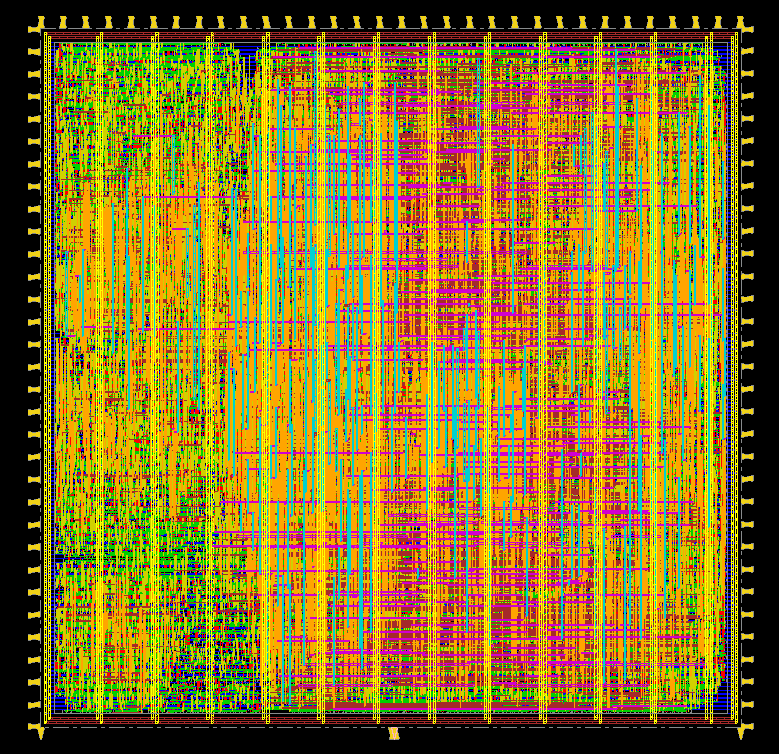
\includegraphics[width=.9\textwidth]{chapters/9_PhysicalDesign/images/pre_routing.png}
        \caption{DLX processor before routing, only logical connections are present}
        \label{fig:pre_routing}
    \end{subfigure}\hfill
    \begin{subfigure}[t]{.45\textwidth}
        \centering
        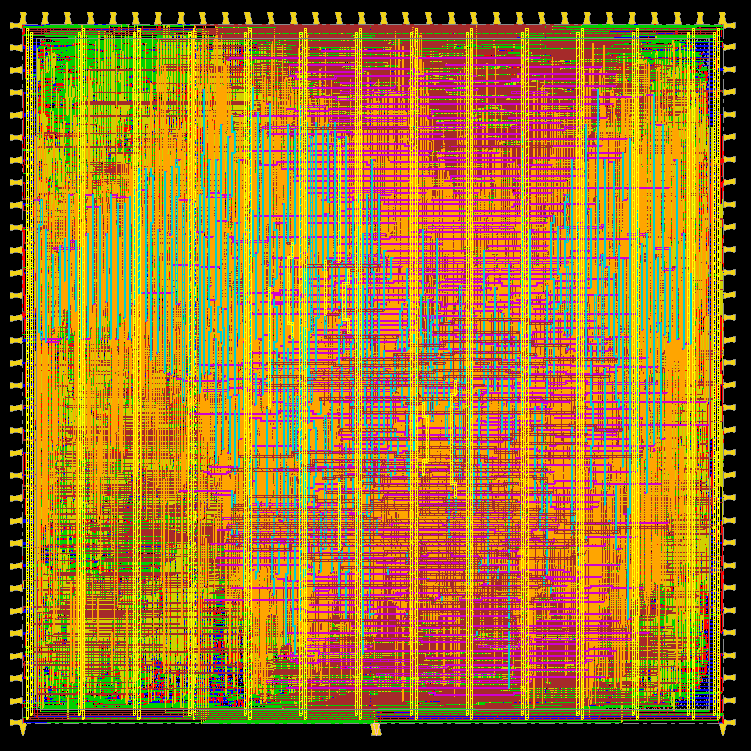
\includegraphics[width=.9\textwidth]{chapters/9_PhysicalDesign/images/phy_end.png}
        \caption{DLX processor after Place and Route phases}
        \label{fig:phy_end}
    \end{subfigure}
    \caption{DLX Place and Route}
\end{figure}

In order to obtain a fully placed and routed DLX, many steps are performed:
\begin{itemize}
    \item Structuring the Floorplan: in this step the Verilog file has been loaded using a global file called \texttt{DLX.globals} and a specif amount of internal area is dedicated to the core, while the external one is used for the power rings;
    \item Power distribution: around the core, two metal rings have been located for distributing the power supply, so both GND and $V_{dd}$. This is not enough since the power and ground signals must be correctly distributed. For this reason, multiple vertical metal wires, called strips, has been added to the physical layout. There is a trade-off in the number of stripes since many of them could lead to some problems during the cells routing. Moreover, horizontal wires have been placed to prepare $V_{dd}$ and GND for the standard cells. The results are visible in Figure \ref{stripes};
    \begin{figure}[h]   
        \centering
        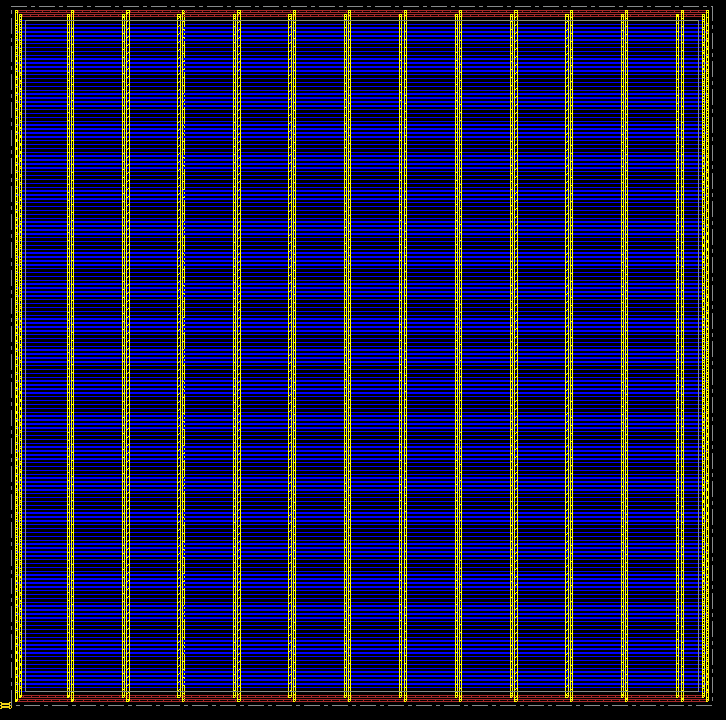
\includegraphics[width=0.38\textwidth]{chapters/9_PhysicalDesign/images/pwr_distribution.png}
        \caption{Result after placing GND and $V_{dd}$ rings with vertical and horizontal stripes.}
        \label{stripes}
    \end{figure}
    
    \item I/O placing: at this point, cells and I/O pins can be placed. Before filling the empty spaces with filler cells a Post Clock-Tree-Synthesis (CTS) optimization has been performed. The result is visible in Figure \ref{fig:pre_routing};
    \item Routing: the last step is the routing; logical interconnections have been replaced with physical interconnections between cells, considering the available stripes and metal rings. The design is now complete, but a post routing optimization has been performed in order to respect the required timing constraints.
\end{itemize}

Once the Place and Route step has been done, a timing analysis has been performed using the \textit{Innovus Debug timing} in order to visualize the delay distribution. The paths delay distributions is visible at \ref{fig:innovus_delay}.
\begin{figure}[h]   
    \centering
    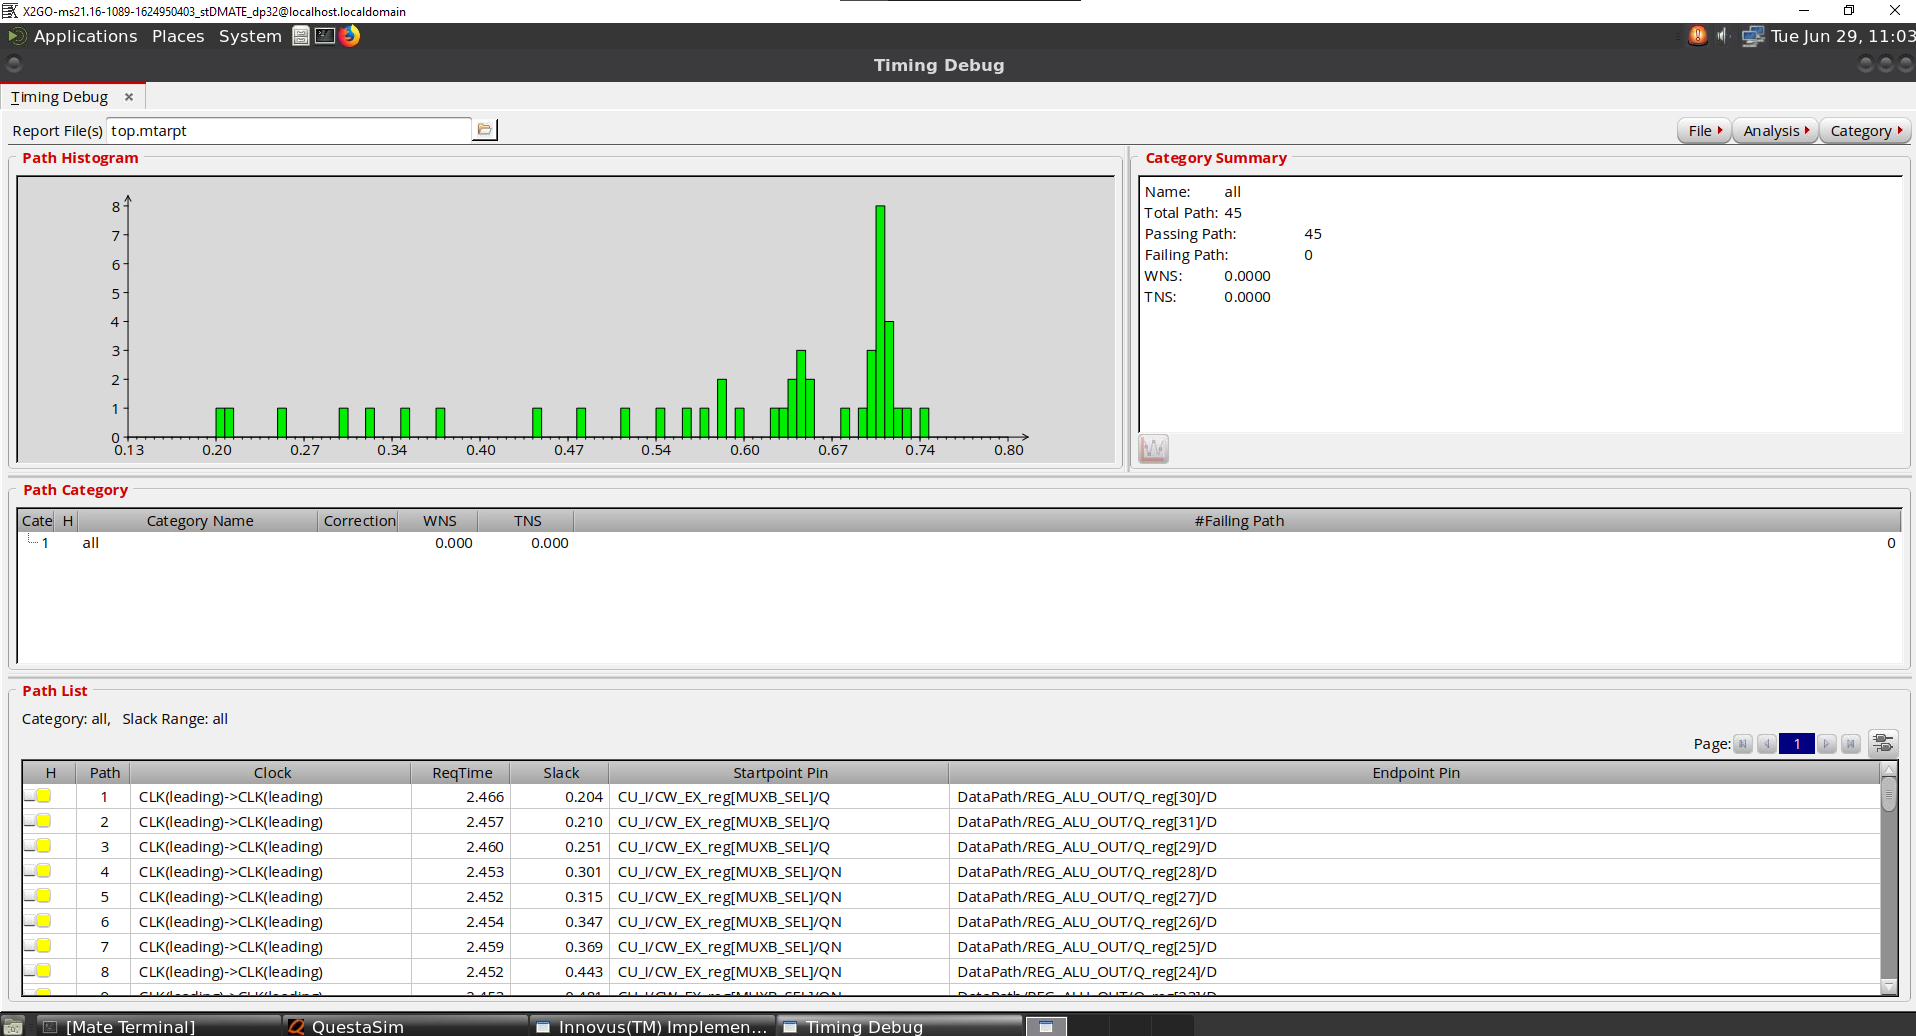
\includegraphics[width=0.8\textwidth]{chapters/9_PhysicalDesign/images/innvous_delay.png}
    \caption{Result after placing GND and $V_{dd}$ rings with vertical and horizontal stripes.}
    \label{fig:innovus_delay}
\end{figure}

Last but not least, before ending the place and route process, design analysis and verification have been performed to ensure that the connectivity and design rules are respected.
\chapter{Conclusions}
To sum up, after the Synthesis and Optimization phase, the peak frequency is 400 MHz. The generated reports highlight that the main power contribution is the dynamic one. This is due to the complex logic that has been implemented in the entire DLX. This DLX implementation has been intensively tested using complex assembly programs, starting from the arithmetic instructions to the sub-routine management.\\

The entire development has been focused on a modular approach to simplify the integration of new components and possible improvements. For example, further improvements could be the management of exceptions, a cache for the instruction and a branch target buffer.\\

All team members contributed actively and with a proactive approach to all the challenges this project brought. \\
\newcommand{\newappendix}{%
	\refstepcounter{chapter}\chapter*{Appendix \thechapter}%
	\addcontentsline{toc}{chapter}{Appendix \thechapter}%
}

\appendix
\newappendix\label{ap1}
\section{ASM compile script}
\begin{lstlisting}[language=bash,caption={Bash script for generating the .mem file from an .asm one},label=code:asm_script]
	#!/bin/sh
	
	if [ ! -r "$1" ]; then
		echo "Usage: $0 <dlx_assembly_file>.asm"
		exit 1
	fi
	
	./assembler.sh $1
	
	filename=$(basename $1)
	filename="${filename%.*}"
		
	assembler.bin/conv2memory ${1%/*}/$filename.bin > DLX_vhd_fully_synthesizable/test_bench_and_memory/mems/${filename}.asm.mem
\end{lstlisting}

\section{Simulation script}
\begin{lstlisting}[language=tcl,caption={Tcl script for staring the simulation and add the registers from R0 to R31},label=sim_wave]
	vcom test_bench_and_memory/TB_TOP_DLX.vhd
	
	vsim -t 10ps work.DLX_TestBench
	log -r *
	
	add wave -position insertpoint sim:/DLX_TestBench/CLK
	
	add wave -position insertpoint sim:/DLX_TestBench/DDLX/DECODEhw/op_code sim:/DLX_TestBench/DDLX/DECODEhw/ADD_RS1 sim:/DLX_TestBench/DDLX/DECODEhw/ADD_RS2 sim:/DLX_TestBench/DDLX/DECODEhw/ADD_WS1
	
	add wave -divider
	add wave -position insertpoint sim:/DLX_TestBench/DDLX/DataPath/RF/DATAIN
	add wave -position insertpoint sim:/DLX_TestBench/DDLX/DataPath/RF/ADD_WR
	
	add wave -position insertpoint -group PROC_REGS -label R0 sim:/DLX_TestBench/DDLX/DataPath/RF/REGS(0)/GLOB_BLK/BLOCK_GLOB/Q
	add wave -position insertpoint -group PROC_REGS -label R1 sim:/DLX_TestBench/DDLX/DataPath/RF/REGS(1)/GLOB_BLK/BLOCK_GLOB/Q
	add wave -position insertpoint -group PROC_REGS -label R2 sim:/DLX_TestBench/DDLX/DataPath/RF/REGS(2)/GLOB_BLK/BLOCK_GLOB/Q
	add wave -position insertpoint -group PROC_REGS -label R3 sim:/DLX_TestBench/DDLX/DataPath/RF/REGS(3)/GLOB_BLK/BLOCK_GLOB/Q
	add wave -position insertpoint -group PROC_REGS -label R4 sim:/DLX_TestBench/DDLX/DataPath/RF/REGS(4)/GLOB_BLK/BLOCK_GLOB/Q
	add wave -position insertpoint -group PROC_REGS -label R5 sim:/DLX_TestBench/DDLX/DataPath/RF/REGS(5)/GLOB_BLK/BLOCK_GLOB/Q
	add wave -position insertpoint -group PROC_REGS -label R6 sim:/DLX_TestBench/DDLX/DataPath/RF/REGS(6)/GLOB_BLK/BLOCK_GLOB/Q
	add wave -position insertpoint -group PROC_REGS -label R7 sim:/DLX_TestBench/DDLX/DataPath/RF/REGS(7)/GLOB_BLK/BLOCK_GLOB/Q
	
	add wave -position insertpoint -group PROC_REGS -label R8 sim:/DLX_TestBench/DDLX/DataPath/RF/SEL_BLK/curr_proc_regs[31:0]
	add wave -position insertpoint -group PROC_REGS -label R9 sim:/DLX_TestBench/DDLX/DataPath/RF/SEL_BLK/curr_proc_regs[63:32]
	add wave -position insertpoint -group PROC_REGS -label R10 sim:/DLX_TestBench/DDLX/DataPath/RF/SEL_BLK/curr_proc_regs[95:64]
	add wave -position insertpoint -group PROC_REGS -label R11 sim:/DLX_TestBench/DDLX/DataPath/RF/SEL_BLK/curr_proc_regs[127:96]
	add wave -position insertpoint -group PROC_REGS -label R12 sim:/DLX_TestBench/DDLX/DataPath/RF/SEL_BLK/curr_proc_regs[159:128]
	add wave -position insertpoint -group PROC_REGS -label R13 sim:/DLX_TestBench/DDLX/DataPath/RF/SEL_BLK/curr_proc_regs[191:160]
	add wave -position insertpoint -group PROC_REGS -label R14 sim:/DLX_TestBench/DDLX/DataPath/RF/SEL_BLK/curr_proc_regs[223:192]
	add wave -position insertpoint -group PROC_REGS -label R15 sim:/DLX_TestBench/DDLX/DataPath/RF/SEL_BLK/curr_proc_regs[255:224]
	add wave -position insertpoint -group PROC_REGS -label R16 sim:/DLX_TestBench/DDLX/DataPath/RF/SEL_BLK/curr_proc_regs[287:256]
	add wave -position insertpoint -group PROC_REGS -label R17 sim:/DLX_TestBench/DDLX/DataPath/RF/SEL_BLK/curr_proc_regs[319:288]
	add wave -position insertpoint -group PROC_REGS -label R18 sim:/DLX_TestBench/DDLX/DataPath/RF/SEL_BLK/curr_proc_regs[351:320]
	add wave -position insertpoint -group PROC_REGS -label R19 sim:/DLX_TestBench/DDLX/DataPath/RF/SEL_BLK/curr_proc_regs[383:352]
	add wave -position insertpoint -group PROC_REGS -label R20 sim:/DLX_TestBench/DDLX/DataPath/RF/SEL_BLK/curr_proc_regs[415:384]
	add wave -position insertpoint -group PROC_REGS -label R21 sim:/DLX_TestBench/DDLX/DataPath/RF/SEL_BLK/curr_proc_regs[447:416]
	add wave -position insertpoint -group PROC_REGS -label R22 sim:/DLX_TestBench/DDLX/DataPath/RF/SEL_BLK/curr_proc_regs[479:448]
	add wave -position insertpoint -group PROC_REGS -label R23 sim:/DLX_TestBench/DDLX/DataPath/RF/SEL_BLK/curr_proc_regs[511:480]
	add wave -position insertpoint -group PROC_REGS -label R24 sim:/DLX_TestBench/DDLX/DataPath/RF/SEL_BLK/curr_proc_regs[543:512]
	add wave -position insertpoint -group PROC_REGS -label R25 sim:/DLX_TestBench/DDLX/DataPath/RF/SEL_BLK/curr_proc_regs[575:544]
	add wave -position insertpoint -group PROC_REGS -label R26 sim:/DLX_TestBench/DDLX/DataPath/RF/SEL_BLK/curr_proc_regs[607:576]
	add wave -position insertpoint -group PROC_REGS -label R27 sim:/DLX_TestBench/DDLX/DataPath/RF/SEL_BLK/curr_proc_regs[639:608]
	add wave -position insertpoint -group PROC_REGS -label R28 sim:/DLX_TestBench/DDLX/DataPath/RF/SEL_BLK/curr_proc_regs[671:640]
	add wave -position insertpoint -group PROC_REGS -label R29 sim:/DLX_TestBench/DDLX/DataPath/RF/SEL_BLK/curr_proc_regs[703:672]
	add wave -position insertpoint -group PROC_REGS -label R30 sim:/DLX_TestBench/DDLX/DataPath/RF/SEL_BLK/curr_proc_regs[735:704]
	add wave -position insertpoint -group PROC_REGS -label R31 sim:/DLX_TestBench/DDLX/DataPath/RF/SEL_BLK/curr_proc_regs[767:736]
\end{lstlisting}
	
\newappendix\label{ap2}
\section{Bash synthesis script}
\begin{lstlisting}[language=bash,caption={Bash script for the DLX synthesis},label=bash_syn]
	#!/bin/sh
		
	source /software/scripts/init_synopsys_64.11
	
	cp ../.synopsys_dc.setup ./
	cp -r ../alib-52 ./
	dc_shell -no_log -f synthesis.script
	
	rm -rf rm -rf ARCH/ BODY/ ENTI/ PACK/
	rm -rf alib-52
	rm -f *.mr
	rm -f ./.synopsys_dc.setup 
	rm -f default.svf
	
	mv DLX_SYN.vhdl ./synthesis_result
	mv DLX_SYN.v ./synthesis_result
	mv dlx_sdf.sdf ./synthesis_result
	mv dlx_sdc.sdc ./synthesis_result
	mv report_*.txt ./synthesis_result
\end{lstlisting}

\section{Synthesis script}
\begin{lstlisting}[language=tcl,caption={TCL script for the DLX synthesis},label=tcl_syn]
	analyze -library WORK -format vhdl {
		./000-globals.vhd
		./001-globals_CU.vhd
		./a.b-DataPath.core/a.b.a-windowedRF.core/a.b.a.m-utils.vhd
		./a.b-DataPath.core/a.b.a-windowedRF.core/a.b.a.a-addr_encoder.vhd
		./a.b-DataPath.core/a.b.a-windowedRF.core/a.b.a.b-address_generator.vhd
		./a.b-DataPath.core/a.b.a-windowedRF.core/a.b.a.c-connection_mtx.vhd
		./a.b-DataPath.core/a.b.a-windowedRF.core/a.b.a.d-decoder.vhd
		./a.b-DataPath.core/a.b.a-windowedRF.core/a.b.a.e-equal_check.vhd
		./a.b-DataPath.core/a.b.a-windowedRF.core/a.b.a.f-in_loc_selblock.vhd
		./a.b-DataPath.core/a.b.a-windowedRF.core/a.b.a.g-mux.vhd
		./a.b-DataPath.core/a.b.a-windowedRF.core/a.b.a.h-nwin_calc.vhd
		./a.b-DataPath.core/a.b.a-windowedRF.core/a.b.a.i-reg_generic.vhd
		./a.b-DataPath.core/a.b.a-windowedRF.core/a.b.a.l-select_block.vhd
		./a.b-DataPath.core/a.b.a-windowedRF.core/a.b.a.n-latch_generic.vhd
		./a.b-DataPath.core/a.b.a-windowedRF.vhd
		./a.b-DataPath.core/a.b.b-mux2to1.vhd
		./a.b-DataPath.core/a.b.d-ALU.core/a.b.d.a-logic.vhd
		./a.b-DataPath.core/a.b.d-ALU.core/a.b.d.b-multiplier.core/a.b.d.b.a-adder.vhd
		./a.b-DataPath.core/a.b.d-ALU.core/a.b.d.b-multiplier.core/a.b.d.b.b-encoder.vhd
		./a.b-DataPath.core/a.b.d-ALU.core/a.b.d.b-multiplier.core/a.b.d.b.c-mux3_1.vhd
		./a.b-DataPath.core/a.b.d-ALU.core/a.b.d.b-multiplier.vhd
		./a.b-DataPath.core/a.b.d-ALU.core/a.b.d.c-adder.core/a.b.d.c.a-carry_generator.vhd
		./a.b-DataPath.core/a.b.d-ALU.core/a.b.d.c-adder.core/a.b.d.c.b-carry_select_block.vhd
		./a.b-DataPath.core/a.b.d-ALU.core/a.b.d.c-adder.core/a.b.d.c.d-fa.vhd
		./a.b-DataPath.core/a.b.d-ALU.core/a.b.d.c-adder.core/a.b.d.c.e-GG.vhd
		./a.b-DataPath.core/a.b.d-ALU.core/a.b.d.c-adder.core/a.b.d.c.f-mux21_generic.vhd
		./a.b-DataPath.core/a.b.d-ALU.core/a.b.d.c-adder.core/a.b.d.c.g-PG.vhd
		./a.b-DataPath.core/a.b.d-ALU.core/a.b.d.c-adder.core/a.b.d.c.h-prop_gen.vhd
		./a.b-DataPath.core/a.b.d-ALU.core/a.b.d.c-adder.core/a.b.d.c.i-prop_gen_generic.vhd
		./a.b-DataPath.core/a.b.d-ALU.core/a.b.d.c-adder.core/a.b.d.c.l-rca_generic.vhd
		./a.b-DataPath.core/a.b.d-ALU.core/a.b.d.c-adder.core/a.b.d.c.m-sum_generator.vhd
		./a.b-DataPath.core/a.b.d-ALU.core/a.b.d.c-adder.vhd
		./a.b-DataPath.core/a.b.d-ALU.core/a.b.d.e-shifter.vhd
		./a.b-DataPath.core/a.b.d-ALU.vhd
		./a.b-DataPath.core/a.b.e-wRF_CU.vhd
		./a.b-DataPath.core/a.b.f-set_comparator.vhd
		./a.b-DataPath.core/a.b.g-datamem_ldstr.vhd
		./a.b-DataPath.core/a.b.h-addr_mask.vhd
		./a.b-DataPath.vhd
		./a.d-decode.core/a.d.a-hazard_table.vhd
		./a.d-decode.core/a.d.b-comparator.vhd
		./a.d-decode.core/a.d.c-ha_counter.vhd
		./a.d-decode.vhd
		./a.a-CU_HW.vhd
		./a-DLX.vhd
	}
	
	elaborate DLX -architecture dlx_rtl -library WORK -parameters "IR_SIZE = 32, PC_SIZE = 32, RAM_DEPTH = 32"
	
	set_wire_load_model -name 5K_hvratio_1_4
	create_clock -name "CLK" -period 2.47 CLK
	
	compile_ultra -timing_high_effort_script
	
	write -hierarchy -format vhdl -output ./DLX_SYN.vhdl
	write -hierarchy -format verilog -output ./DLX_SYN.v
	write_sdf dlx_sdf.sdf
	write_sdc dlx_sdc.sdc
	
	report_timing > report_timing.txt
	report_area > report_area.txt
	report_power > report_power.txt
	
	exit
\end{lstlisting}


\newappendix\label{ap3}
\section{Area report}
\begin{lstlisting}
	 
	****************************************
	Report : area
	Design : DLX_IR_SIZE32_PC_SIZE32_RAM_DEPTH32
	Version: F-2011.09-SP3
	Date   : Fri Jul 16 16:59:22 2021
	****************************************
	
	Library(s) Used:
	
	NangateOpenCellLibrary (File: /home/mariagrazia.graziano/do/libnangate/NangateOpenCellLibrary_typical_ecsm.db)
	
	Number of ports:                          270
	Number of nets:                         14478
	Number of cells:                        12492
	Number of combinational cells:           9127
	Number of sequential cells:              3360
	Number of macros:                           0
	Number of buf/inv:                       1016
	Number of references:                      66
	
	Combinational area:       19748.904346
	Noncombinational area:    15531.473475
	Net Interconnect area:      undefined  (Wire load has zero net area)
	
	Total cell area:          35280.377821
	Total area:                 undefined
\end{lstlisting}


\section{Power report}
\begin{lstlisting}
	****************************************
	Report : power
	-analysis_effort low
	Design : DLX_IR_SIZE32_PC_SIZE32_RAM_DEPTH32
	Version: F-2011.09-SP3
	Date   : Fri Jul 16 16:59:26 2021
	****************************************
	
	
	Library(s) Used:
	
	NangateOpenCellLibrary (File: /home/mariagrazia.graziano/do/libnangate/NangateOpenCellLibrary_typical_ecsm.db)
	
	
	Operating Conditions: typical   Library: NangateOpenCellLibrary
	Wire Load Model Mode: top
	
	Design        Wire Load Model            Library
	------------------------------------------------
	DLX_IR_SIZE32_PC_SIZE32_RAM_DEPTH32
	5K_hvratio_1_4    NangateOpenCellLibrary
	
	
	Global Operating Voltage = 1.1  
	Power-specific unit information :
	Voltage Units = 1V
	Capacitance Units = 1.000000ff
	Time Units = 1ns
	Dynamic Power Units = 1uW    (derived from V,C,T units)
	Leakage Power Units = 1nW
	
	
	Cell Internal Power  =   9.5411 mW   (95%)
	Net Switching Power  = 474.3534 uW    (5%)
	---------
	Total Dynamic Power    =  10.0154 mW  (100%)
	
	Cell Leakage Power     = 657.4517 uW
	
	
	Internal         Switching           Leakage            Total
	Power Group      Power            Power               Power              Power   (   %    )  Attrs
	--------------------------------------------------------------------------------------------------
	io_pad             0.0000            0.0000            0.0000            0.0000  (   0.00%)
	memory             0.0000            0.0000            0.0000            0.0000  (   0.00%)
	black_box          0.0000            0.0000            0.0000            0.0000  (   0.00%)
	clock_network      0.0000            0.0000            0.0000            0.0000  (   0.00%)
	register       9.3982e+03           16.0318        2.6602e+05        9.6802e+03  (  90.70%)
	sequential        12.6095            0.7893        3.1563e+03           16.5551  (   0.16%)
	combinational    130.4222          457.5387        3.8827e+05          976.2318  (   9.15%)
	--------------------------------------------------------------------------------------------------
	Total          9.5412e+03 uW       474.3597 uW     6.5744e+05 nW     1.0673e+04 uW
\end{lstlisting}


\section{Timing report}
\begin{lstlisting}
	 
	****************************************
	Report : timing
	-path full
	-delay max
	-max_paths 1
	Design : DLX_IR_SIZE32_PC_SIZE32_RAM_DEPTH32
	Version: F-2011.09-SP3
	Date   : Fri Jul 16 16:59:22 2021
	****************************************
	
	# A fanout number of 1000 was used for high fanout net computations.
	
	Operating Conditions: typical   Library: NangateOpenCellLibrary
	Wire Load Model Mode: top
	
	Startpoint: CU_I/CW_EX_reg[MUXB_SEL]
	(rising edge-triggered flip-flop clocked by CLK)
	Endpoint: DataPath/REG_ALU_OUT/Q_reg[31]
	(rising edge-triggered flip-flop clocked by CLK)
	Path Group: CLK
	Path Type: max
	
	Des/Clust/Port     Wire Load Model       Library
	------------------------------------------------
	DLX_IR_SIZE32_PC_SIZE32_RAM_DEPTH32
	5K_hvratio_1_4        NangateOpenCellLibrary
	
	Point                                                   Incr       Path
	--------------------------------------------------------------------------
	clock CLK (rise edge)                                   0.00       0.00
	clock network delay (ideal)                             0.00       0.00
	CU_I/CW_EX_reg[MUXB_SEL]/CK (DFF_X1)                    0.00 #     0.00 r
	CU_I/CW_EX_reg[MUXB_SEL]/QN (DFF_X1)                    0.07       0.07 r
	U9386/ZN (INV_X1)                                       0.04       0.11 f
	U11439/ZN (NAND2_X1)                                    0.04       0.15 r
	U8853/ZN (NAND2_X1)                                     0.04       0.19 f
	U8919/ZN (INV_X1)                                       0.05       0.24 r
	U9225/Z (BUF_X1)                                        0.11       0.36 r
	U8950/ZN (INV_X1)                                       0.06       0.41 f
	U8949/ZN (XNOR2_X1)                                     0.08       0.49 f
	U8993/ZN (XNOR2_X1)                                     0.07       0.56 f
	DP_OP_751_130_6421/U1157/S (FA_X1)                      0.14       0.70 r
	DP_OP_751_130_6421/U1089/S (FA_X1)                      0.12       0.81 f
	DP_OP_751_130_6421/U1021/CO (FA_X1)                     0.10       0.91 f
	DP_OP_751_130_6421/U952/S (FA_X1)                       0.15       1.06 r
	DP_OP_751_130_6421/U884/S (FA_X1)                       0.12       1.18 f
	DP_OP_751_130_6421/U816/S (FA_X1)                       0.14       1.32 r
	DP_OP_751_130_6421/U748/S (FA_X1)                       0.12       1.43 f
	DP_OP_751_130_6421/U680/S (FA_X1)                       0.14       1.57 r
	DP_OP_751_130_6421/U612/S (FA_X1)                       0.12       1.69 f
	U9220/ZN (OR2_X1)                                       0.07       1.75 f
	U9221/ZN (AOI21_X1)                                     0.06       1.81 r
	U9222/ZN (OAI21_X1)                                     0.04       1.85 f
	U8972/ZN (NAND2_X1)                                     0.03       1.88 r
	U8971/ZN (NAND2_X1)                                     0.03       1.92 f
	U9058/ZN (NAND2_X1)                                     0.03       1.95 r
	U9101/ZN (NAND2_X1)                                     0.03       1.98 f
	U9099/ZN (NAND2_X1)                                     0.03       2.01 r
	U9097/ZN (NAND2_X1)                                     0.03       2.04 f
	U9093/ZN (NAND2_X1)                                     0.03       2.07 r
	U9043/ZN (NAND2_X1)                                     0.03       2.10 f
	U9041/ZN (NAND2_X1)                                     0.03       2.13 r
	U8936/ZN (NAND2_X1)                                     0.03       2.16 f
	U8340/ZN (NAND2_X1)                                     0.04       2.20 r
	U8337/ZN (NAND3_X1)                                     0.03       2.23 f
	U8324/ZN (AND2_X1)                                      0.04       2.28 f
	U8323/ZN (AOI21_X1)                                     0.05       2.32 r
	U8320/ZN (XNOR2_X1)                                     0.06       2.39 r
	U8319/ZN (OAI21_X1)                                     0.03       2.42 f
	DataPath/REG_ALU_OUT/Q_reg[31]/D (DFF_X1)               0.01       2.43 f
	data arrival time                                                  2.43
	
	clock CLK (rise edge)                                   2.47       2.47
	clock network delay (ideal)                             0.00       2.47
	DataPath/REG_ALU_OUT/Q_reg[31]/CK (DFF_X1)              0.00       2.47 r
	library setup time                                     -0.04       2.43
	data required time                                                 2.43
	--------------------------------------------------------------------------
	data required time                                                 2.43
	data arrival time                                                 -2.43
	--------------------------------------------------------------------------
	slack (MET)                                                        0.00
\end{lstlisting}

\newappendix\label{asm_examples}

\section{Finonacci Code}

\begin{lstlisting}[style=mips,caption={Fibonacci DLX Assembly example},label=asm_fibonacci]
addi r24, r0, #6

call fib
j exit

fib:    ; N is on r8, result in r9
    addi r16, r0, #1
    ble r8, r16, ret_1

    subi r24, r8, #1
    call fib ; n-1

    add r9, r25, r0   
    subi r24, r8, #2

    call fib ; n-2

    add r9, r9, r25       
    ret

ret_1:
    ; if n == 0 -> 0
    ; if n == 1 -> 1
    beqz r8, zero

    addi r9, r0, #1
    j out
    
zero:
    add r9, r0, r0

out:
    ret   

exit:

    sw 0(r0), r25

    j exit

\end{lstlisting}

\newpage
\section{Factorial Code}

\begin{lstlisting}[style=mips,caption={Factorial DLX Assembly example},label=asm_factorial]
addi r24, r0, #10           ;0

ticktmr r16                 ;4
call fact                   ;8
ticktmr r17                 ;C

j exit                      ;10


; R8 => INPUT for current call from prev call
; R9 => OUTPUT for current call towards prev call
; R24 => INPUT FOR NEXT CALL
; R25 => OUTPUT FROM LAST CALL
fact:
    seqi r16, r8, #1        ;14
    bnez r16, end           ;18

    ; continue rec
    ; n * call fact(n-1)
    subi r24, r8, #1      ; n = n-1         ;1C
    call fact               ;20 
    mult r9, r8, r25        ;24
    ret                     ;28
 
 end:
    addi r9, r0, #1         ;2C
    ret                     ;30

exit:
    sw 0(r0), r25   ; store result
    
    sub r17, r17, r16 ; total elapsed time (end - start)
    sw 16(r0), r17  ; store elaps time

halt:
    j halt

\end{lstlisting}


\newpage
\section{Bubble Sort Code}

\begin{lstlisting}[style=mips,caption={Bubble Sort DLX Assembly example},label=asm_bubble_sort]
.text

j start_code

swap: ; r8 <- array, r9 <- j
	slli r20, r9, #2
	add r17, r8, r20	; ptr to array + j
	lw r18, 0(r17)	
	lw r19, 4(r17)
	ble r18, r19, not_swap
	; swap here
	sw 0(r17), r19
	sw 4(r17), r18
	addi r1, r0, #1	; swapped = true

not_swap:
	ret	


bubbleSort: ;R8 <- N, R9 <- array

subi R8, R8, #1	; r1 <- N--
addi r17, r0, #0	; index i
fori:
	addi r1, r0, #0 	; swapped = false, global
	addi r19, r0, #0	; index j
	sub r20, r8, r17	; r20 <- n-1-i
	forj:
		add r24, r0, r9 	; arg #0 : ptr
		add r25, r0, r19	; arg #2 : index j
		call swap

		addi r19, r19, #1	;j++
		seq r18, r19, r20	; if j == n-i-1 
		bnez r18, exit_forj
		j forj


	exit_forj:
		beqz r1, end_sort 

		addi r17, r17, #1	; i++
		seq r18, r17, r8	; if i == n-1
		bnez r18, end_sort
		j fori
	

end_sort:
	ret

start_code:
	addi r24, r0, #12 ; N
	lw r25, array_0(r0)
	call bubbleSort
	
stop:
	j stop	





;###############
; DATA SEGMENT #
;###############

	.data

code_space:
	.space 256

; The available assembler assigns addresses starting from zero each time
; it finds a new segment. In this way data and text segments are going to 
; overlap and their addresses cannot be shared. To avoid this problem we 
; need to generate absolute code in which starting address of data segment
; is located after last address of text segment. Therefore we use a trick 
; reserving the first part of data segment (code_space) to empty space while
; all useful data structures are defined soon after. In this way, when 
; compiling, the text segment would overlap the data segment just for this
; initial empty space so that as result we have the compiled code followed
; by useful data addresses. Obviously the size of code_space has to be enough
; to contain all compiled code (256 byte are more than enough). 
; array to be sorted

array:
	.word 3,18,-12,24,17,1,7,3,-8,20,100,-33

array_0:
	.word array
\end{lstlisting}

\section{Advanced Branch Code}

\begin{lstlisting}[style=mips,caption={Advanced Branch Code DLX Assembly example},label=asm_Advanced_Branch_Code]

a:
    addi r1, r0, #1 ; 1
    addi r3, r0, #4 ; 1
    ble r3, r1, c ; 8
    bge r1, r3, c
    beqz r1, c

b:
    addi r5, r0, #12312 ;10
    blt r3, r1, d
    bgt r3, r1, d

c:
    addi r6, r0, #8 ;18
    jal a

d:
    bge r1, r1, e
    j b

e:
    addi r7, r0, #7
    bge r0, r0, a

\end{lstlisting}


\section{Complete Arithmetic Instructions Code}

\begin{lstlisting}[style=mips,caption={Complete Arithmetic Instructions DLX Assembly example},label=asm_arithms]

	nop
	addi r1,r0,#2       ;2          ;2
	subi r2,r1,#1       ;1          ;1
	addi r3,r1,#-4      ;-2         ;-2
	subi r4,r3,#-1      ;-1
	add r7,r1,r2        ;3
	sub r8,r5,r6        ;0
	sge r10,r1,r2       ;1
	sge r11,r2,r1       ;0
	sge r12,r1,r1       ;1
	sle r13,r1,r2       ;0
	sle r14,r2,r1       ;1
	sle r15,r1,r1       ;1
	sne r16,r1,r1       ;0
	sne r17,r1,r2       ;1
	seq r18,r1,r2       ;0
	seq r19,r1,r1       ;1
	sgt r10,r2,r1       ;0
	sgt r11,r1,r2       ;1
	slt r12,r2,r1       ;1
	slt r10,r1,r2       ;0  2 < 1 
	sgeu r10,r1,r3      ;0  2 >= 654..
	sgeu r11,r3,r1      ;1
	sgtu r12,r1,r3      ;0
	sgtu r13,r3,r1      ;1
	sltu r14,r3,r1      ;0
	sltu r15,r1,r3      ;1
	sgei r16,r1,#4      ;0
	sgei r17,r1,#1      ;1
	slei r18,r1,#0      ;0
	slei r19,r1,#2      ;1
	snei r10,r1,#1      ;1
	snei r11,r1,#2      ;0
	seqi r12,r1,#0      ;0
	seqi r13,r1,#2      ;1
	sgti r14,r1,#3      ;0
	sgti r15,r1,#1      ;1
	slti r16,r1,#1      ;0
	slti r17,r1,#3      ;1
	sgeui r10,r1,#4     ;0
	sgeui r10,r1,#-4    ;0 
	sgeui r11,r1,#1     ;1
	sgtui r12,r1,#3     ;0
	sgtui r13,r1,#1     ;1
	sltui r14,r1,#1     ;0
	sltui r15,r1,#3     ;1
	addi r12,r0,#5      ;5
	or r13,r11,r12      ;5
	ori r14,r12,#65535  ;0000FFFF
	and r15,r14,r2      ;1
	andi r16,r14,#1     ;1
	sll r17,r16,r2      ;2
	slli r18,r16,#1     ;2
	srl r19,r16,r2      ;0
	srli r20,r16,#1     ;0
	sra r21,r12,r2      ;2
	srai r22,r12,#1     ;2
	mult r23,r1,r5      ;0
	xor r24,r1,r1       ;0
	;xori r25, r1, #0xf  ;14

	addi r6, r0, #5     ;5
	addi r1, r0, #2     ;2
	ror r30, r6, r1      ;0100 0000 0000 0000 0000 ... 0001
	addi r7, r0, #5     ;5
	rol r29, r7, r1     ;0000 0000 0000 0000 ... 0001 0100

	addui r28, r0, #0xffff  ; 0x0000ffff
	subui r28, r0, #0xffff  ; 0xffff0001

	lhi r28, #-40           ; 0xfffd8000

	sw 0(r0), r14
	lh r27, 2(r0)       ;ffffffff
	lhu r26, 2(r0)      ;0000ffff

	nop
halt:
	j halt

\end{lstlisting}


\section{Load \& Store Code}

\begin{lstlisting}[style=mips,caption={Load \& Store DLX Assembly example},label=asm_ldstr]

myloop:
    addi r1, r0, #4                      ;0
    addi r8, r0, #10                     ;4
    sw 4(r1), r8                        ;8
    
    addi r9, r0, #-10                    ;C
    sh 5(r1), r9                        ;10
    lb r10, 5(r1)                       ;14
    lbu r11, 5(r1)                      ;18
    lhu r11, 5(r1)                      ;1C
    addi r10, r10, #1                    ;20

    lbu r2, 5(r1)                        ;24
    sh 20(r1), r2                       ;28
    
    lh r3, 20(r1)                        ;2C
    lhi r3, #9                           ;30
    
    addi r4, r5, #15                     ;34
    addi r7, r0, myloop                 ;38
    
    jal myloop        	                ;3C
                                        ;40

\end{lstlisting}





\newappendix\label{ap4}
\section{Windowing Register File}
 \mbox{} \begin{center}
	\begin{sideways}
		\begin{minipage}{1\linewidth}
			\includegraphics[width=1\textwidth]{chapters/11_Appendix/images/wrf.pdf}
			\captionof{figure}{Complete and exhaustive Windowing Register File}
			\label{figure:wrf_complex}
		\end{minipage}
	\end{sideways}
\end{center}


\appendix
% \input{./Appendix/appendix1.tex}
% and so on
%
%%%%%%%%%%%%%%%%%%%%%%%%%%%%%%%%%%%%%%%%%%%%%%%%%%%%%%

\end{document}